\documentclass[preprint,12pt]{elsarticle}

\usepackage{amsmath,amssymb,mathtools}
\usepackage{booktabs}
\usepackage{subcaption}
\usepackage{graphicx}
\usepackage{natbib}
\setlength{\emergencystretch}{2em}

\journal{Electric Power Systems Research}

\begin{document}
\begin{frontmatter}

\title{Nonlinear Observer-Based Control Paradigms for a Two-Stage Grid-Connected PV System}

\author{Noman Ali}
\author{Qudrat Khan}
\author{Waqar Alam}

\affiliation{organization={Department of Electrical Engineering, COMSATS University Islamabad},
            city={Islamabad},
            postcode={44000},
            country={Pakistan}}

\affiliation{organization={Department of Electronics, University of Buner},
            city={Sowari, Buner},
            postcode={19290},
            country={Pakistan}}

\begin{abstract}
The variable nature of solar irradiance and temperature affects the voltage, current, and power generated by photovoltaic (PV) arrays, thereby requiring robust control for reliable grid integration. This study investigates two nonlinear sliding-mode control strategies, namely the continuous twisting algorithm (CTA) and discontinuous integral control (DIC), for a two-stage grid-connected PV system. At the DC--DC conversion stage, a perturb and observe (P\&O) algorithm generates the reference PV voltage, while the CTA and DIC controllers regulate the boost-converter duty cycle to track this reference. At the inverter stage, an outer proportional--integral controller regulates the DC-link voltage and generates the $d$-axis grid-current reference, while the $q$-axis reference is set to zero to limit reactive-power exchange. The CTA and DIC schemes regulate the grid currents in the synchronous $dq$ reference frame. An Utkin sliding-mode observer estimates the filter-capacitor voltages and inverter-side currents required for controller implementation. MATLAB/Simulink results under varying irradiance show dynamic MPPT efficiencies of $99.4\%$, $98.0\%$, and $95.0\%$ for the CTA, DIC, and conventional PI controllers, respectively. The corresponding reported grid-current total harmonic distortion values are $0.43\%$, $0.82\%$, and $2.27\%$. Under the stated matching, disturbance, and gain conditions, the proposed controllers provide finite-time convergence of the MPPT tracking error and finite-time reaching of the inverter sliding manifolds, followed by exponential convergence of the grid-current tracking errors.
\end{abstract}

\begin{keyword}
Grid-connected PV system \sep Continuous twisting algorithm \sep Discontinuous integral control \sep Maximum power point tracking \sep Sliding-mode observer \sep Total harmonic distortion
\end{keyword}

\end{frontmatter}

\section{Introduction}
\label{sec:introduction}

The global transition toward renewable energy sources has emphasized the importance of clean and sustainable power-generation technologies. Among the available renewable energy technologies, photovoltaic (PV) systems have gained considerable attention because they provide a reliable and environmentally friendly means of electricity generation. As countries pursue carbon-neutrality targets, PV systems can contribute to reducing greenhouse-gas emissions and mitigating the adverse effects of climate change \cite{esram2007comparison}. The growing demand for renewable energy is driven by technological advancements and increased awareness of the environmental consequences of fossil-fuel consumption. Unlike conventional fossil-fuel-based generation, PV systems produce electricity without directly emitting harmful pollutants during operation, making them an important component of modern sustainable energy systems \cite{saleh2024challenges}.

The substantial reduction in the cost of PV panels has made solar energy increasingly accessible to residential, commercial, and utility-scale users \cite{nikolina2016international,khan2024economics}. This reduction has resulted from improvements in manufacturing processes, economies of scale, and increased competition among manufacturers \cite{esram2007comparison}. Consequently, households, businesses, and utility companies have increasingly integrated PV-based energy solutions into their operations, thereby accelerating the global adoption of solar energy.

PV systems can generally be classified as either stand-alone or grid-connected systems. A stand-alone PV system operates independently of the utility grid and typically relies on energy-storage devices, such as battery banks, to maintain a continuous power supply. By contrast, a grid-connected PV system exchanges power directly with the utility grid, allowing surplus energy to be injected into the grid and power to be drawn when PV generation is insufficient. This configuration can reduce or eliminate the need for costly energy-storage components, making grid-connected PV systems a practical solution for various applications \cite{carrasco2006power}.

Grid-connected PV systems can be implemented using either single-stage or two-stage architectures \cite{trujillo2016modeling}. In a single-stage configuration, the PV array is connected directly to the grid through a DC--AC inverter. In a two-stage configuration, a DC--DC converter is placed between the PV array and the inverter. The DC--DC converter performs maximum power point tracking (MPPT), whereas the inverter regulates grid synchronization and power injection \cite{kouro2015grid}. This decoupled structure improves control flexibility, facilitates maximum-energy extraction under varying irradiance, and enhances DC-link voltage regulation.

The principal control objectives of a two-stage grid-connected PV system are to maximize the power extracted from the PV array, regulate the DC-link voltage, reduce harmonics in the inverter output, and ensure efficient power transfer to the utility grid. MPPT is implemented through the DC--DC converter, particularly under varying meteorological conditions \cite{trujillo2016modeling}. On the inverter side, switching harmonics can degrade the quality of the current injected into the grid. Filters such as RL, LC, and LCL configurations are therefore commonly employed. Among these options, the LCL filter provides effective attenuation of high-frequency harmonics; however, its resonance characteristics must be considered during controller design \cite{li2023harmonic}. Accurate regulation of the inverter currents is also required to maximize active-power delivery while minimizing reactive-power exchange with the grid \cite{ahmed2022evaluation}.

Various MPPT techniques have been developed to extract the maximum available power from PV arrays. The incremental-conductance method determines the maximum power point by comparing the incremental and instantaneous conductances of the PV array. The P\&O method periodically perturbs the operating voltage and observes the corresponding change in output power. Although the P\&O method is simple and widely used, its performance may deteriorate under rapidly changing irradiance conditions \cite{soumana2022comparison}.

Sliding-mode control (SMC) strategies have been extensively investigated for improving the robustness of two-stage grid-connected PV systems in the presence of uncertainties and disturbances \cite{liu2022sliding,alnami2024enhanced}. An integral SMC scheme for a two-stage, three-phase, grid-connected PV system was presented in \cite{kihal2018robust}. Sliding-mode controllers were also employed in \cite{dash2022photovoltaic,kumar2015sliding} to improve energy-conversion performance and grid compatibility. The control of grid-connected inverters under unbalanced grid-voltage conditions was investigated in \cite{wu2022sliding}. Other nonlinear control techniques include input--output feedback linearization \cite{parvathy2020modelling}, backstepping-based control \cite{aouadi2018nonlinear,naddami2022nonlinear}, adaptive PI control, adaptive SMC \cite{zeb2021control}, and super-twisting sliding-mode control \cite{zeb2020design,dash2024robust}.

This study develops CTA- and DIC-based controllers for both conversion stages of a two-stage grid-connected PV system. At the first stage, the P\&O algorithm generates the reference PV voltage $V_{\mathrm{ref}}$, and the nonlinear controllers regulate the boost-converter duty cycle. At the second stage, a PI controller regulates the DC-link voltage and generates the $d$-axis grid-current reference. The CTA and DIC schemes then regulate the grid currents in the synchronous $dq$ frame. An Utkin sliding-mode observer estimates the filter-capacitor voltages and inverter-side currents required for controller implementation. The complete system is evaluated in MATLAB/Simulink, and the proposed controllers are compared with a conventional PI controller.

The remainder of this paper is organized as follows. Section~\ref{sec:system} presents the system configuration and mathematical model. Section~\ref{sec:proposed} introduces the proposed control structure. Section~\ref{sec:mppt} describes the MPPT controller design. Section~\ref{sec:observer} presents the Utkin observer. Section~\ref{sec:inverter} develops the inverter controllers. Section~\ref{sec:stability} discusses stability. Section~\ref{sec:results} presents the simulation results, and Section~\ref{sec:comparison} provides a quantitative comparison. Section~\ref{sec:conclusion} concludes the paper.

\section{Overall System Configuration}
\label{sec:system}

The proposed system consists of a PV array, a DC--DC boost converter, a DC-link capacitor, a three-phase inverter, an LCL filter, and the utility grid, as shown in Fig.~\ref{fig:system-overview}. The principal control objectives are to extract the maximum available PV power, regulate the DC-link voltage, and inject high-quality current into the utility grid.

\begin{figure}[htbp]
    \centering
    \includegraphics[width=\linewidth]{two stage control Simple f.png}
    \caption{Overall configuration of the proposed two-stage grid-connected PV system.}
    \label{fig:system-overview}
\end{figure}

\subsection{PV Array}

The single-diode model of the PV array is expressed as
\begin{equation}
I=N_p\left[I_{ph}-I_0\left(\exp\left(\frac{V/N_s+IR_s}{nV_t}\right)-1\right)-\frac{V/N_s+IR_s}{R_{sh}}\right],
\label{eq:pv-model}
\end{equation}
where $I$ and $V$ are the array current and voltage, $I_{ph}$ is the photocurrent, $I_0$ is the diode reverse-saturation current, $R_s$ and $R_{sh}$ are the series and shunt resistances, $n$ is the diode ideality factor, and $N_s$ and $N_p$ are the numbers of series- and parallel-connected cells or modules. The thermal voltage is
\begin{equation}
V_t=\frac{kT}{q},
\end{equation}
where $k$ is the Boltzmann constant, $T$ is the absolute temperature, and $q$ is the elementary charge.

\subsection{Boost Converter}

The averaged boost-converter model is
\begin{equation}
\frac{di_L}{dt}=\frac{V_{pv}}{L_b}-\frac{(1-D)V_{dc}}{L_b},
\label{eq:boost-current}
\end{equation}
\begin{equation}
\frac{dV_{pv}}{dt}=\frac{1}{C_{pv}}\left(I_{pv}-i_L\right),
\label{eq:boost-voltage}
\end{equation}
where $i_L$ is the boost-inductor current, $V_{pv}$ and $I_{pv}$ are the PV-array voltage and current, $V_{dc}$ is the DC-link voltage, $L_b$ is the boost inductance, $C_{pv}$ is the PV-side capacitance, and $D$ is the duty cycle.

\begin{figure}[htbp]
    \centering
    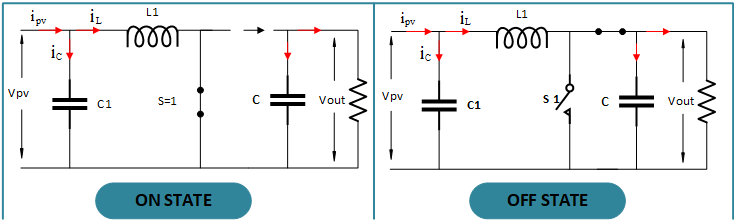
\includegraphics[width=0.48\textwidth]{BOOST Circuit noman.png}
    \caption{Operating states of the boost converter: (a) switch-on state and (b) switch-off state.}
    \label{fig:boost}
\end{figure}

\subsection{Three-Phase Inverter with an LCL Filter}

The inverter is connected to the utility grid through an LCL filter comprising the inverter-side inductance $L_i$, filter capacitance $C_f$, and grid-side inductance $L_g$, as shown in Fig.~\ref{fig:grid-inverter}.

\begin{figure}[htbp]
    \centering
    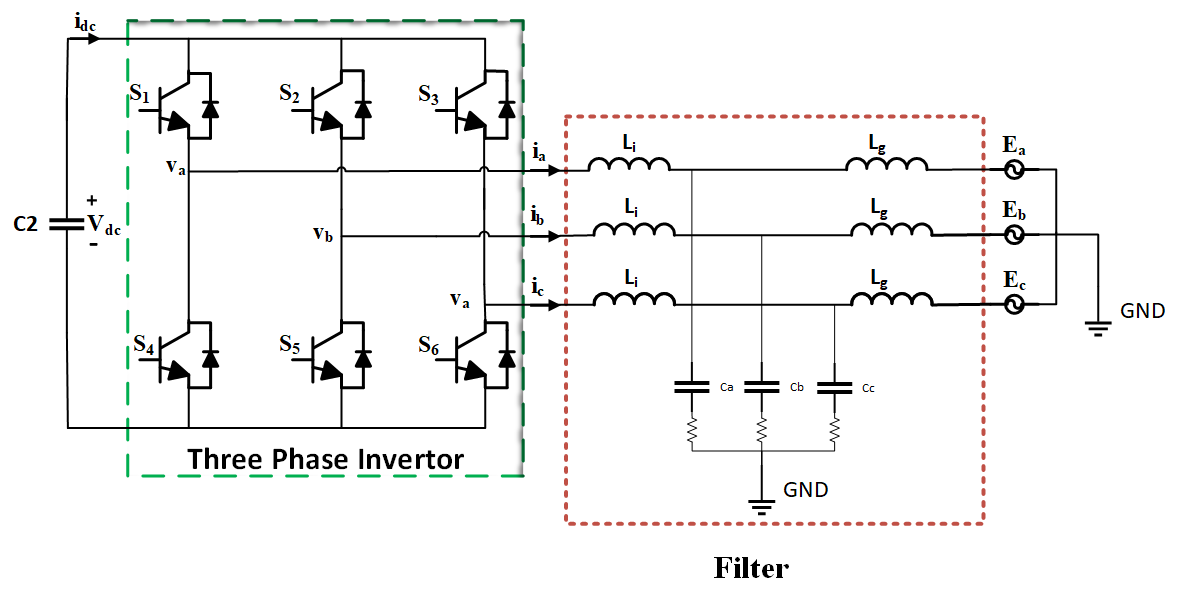
\includegraphics[width=\linewidth]{Grid connected Inverter.png}
    \caption{Three-phase grid-connected inverter with an LCL filter.}
    \label{fig:grid-inverter}
\end{figure}

In the stationary $abc$ frame, the LCL-filter dynamics are
\begin{equation}
\left\{
\begin{aligned}
\frac{di_{g,abc}}{dt}&=\frac{1}{L_g}\left(v_{c,abc}-v_{g,abc}\right),\\
\frac{dv_{c,abc}}{dt}&=\frac{1}{C_f}\left(i_{i,abc}-i_{g,abc}\right),\\
\frac{di_{i,abc}}{dt}&=\frac{1}{L_i}\left(v_{i,abc}-v_{c,abc}\right).
\end{aligned}
\right.
\label{eq:abc-model}
\end{equation}

Using the adopted Park-transformation convention, the synchronous-frame model is
\begin{equation}
\left\{
\begin{aligned}
\dot I_{gd}&=\frac{1}{L_g}V_{cd}+\omega I_{gq}-\frac{1}{L_g}V_{gd},\\
\dot V_{cd}&=\frac{1}{C_f}I_d-\frac{1}{C_f}I_{gd}+\omega V_{cq},\\
\dot I_d&=-\frac{1}{L_i}V_{cd}+\omega I_q+\frac{1}{L_i}V_d,\\
\dot I_{gq}&=\frac{1}{L_g}V_{cq}-\omega I_{gd}-\frac{1}{L_g}V_{gq},\\
\dot V_{cq}&=\frac{1}{C_f}I_q-\frac{1}{C_f}I_{gq}-\omega V_{cd},\\
\dot I_q&=-\frac{1}{L_i}V_{cq}-\omega I_d+\frac{1}{L_i}V_q.
\end{aligned}
\right.
\label{eq:dq-model}
\end{equation}

The state vector is defined as
\begin{equation}
x=\begin{bmatrix}I_{gd}&V_{cd}&I_d&I_{gq}&V_{cq}&I_q\end{bmatrix}^{T}.
\label{eq:state-vector}
\end{equation}

\section{Proposed Control Structure}
\label{sec:proposed}

The control system addresses MPPT at the boost-converter stage and grid-current regulation at the inverter stage. The CTA and DIC controllers are employed at both stages. A PI outer loop regulates the DC-link voltage, and a phase-locked loop supplies the grid angle required for the $dq$ transformations.

For compactness, the signed-power function is defined as
\begin{equation}
\left\lceil z\right\rfloor^{\alpha}=|z|^{\alpha}\operatorname{sign}(z),\qquad \alpha\geq0.
\label{eq:signed-power}
\end{equation}
In particular, $\left\lceil z\right\rfloor^0=\operatorname{sign}(z)$.

\section{Design of the MPPT Controllers}
\label{sec:mppt}

The P\&O algorithm generates $V_{\mathrm{ref}}$, while the CTA or DIC controller regulates $D$ so that $V_{pv}$ follows this reference.

\begin{figure}[htbp]
    \centering
    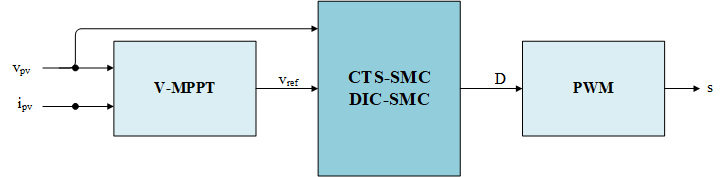
\includegraphics[width=\linewidth]{MPPT.png}
    \caption{Proposed voltage-oriented MPPT control structure.}
    \label{fig:mppt-block}
\end{figure}

\subsection{P\&O-Based Voltage Reference}

The P\&O method periodically perturbs the PV operating voltage and evaluates the resulting change in power. If the perturbation increases the generated power, the operating point is adjusted in the same direction; otherwise, the perturbation direction is reversed.

\begin{figure}[htbp]
    \centering
    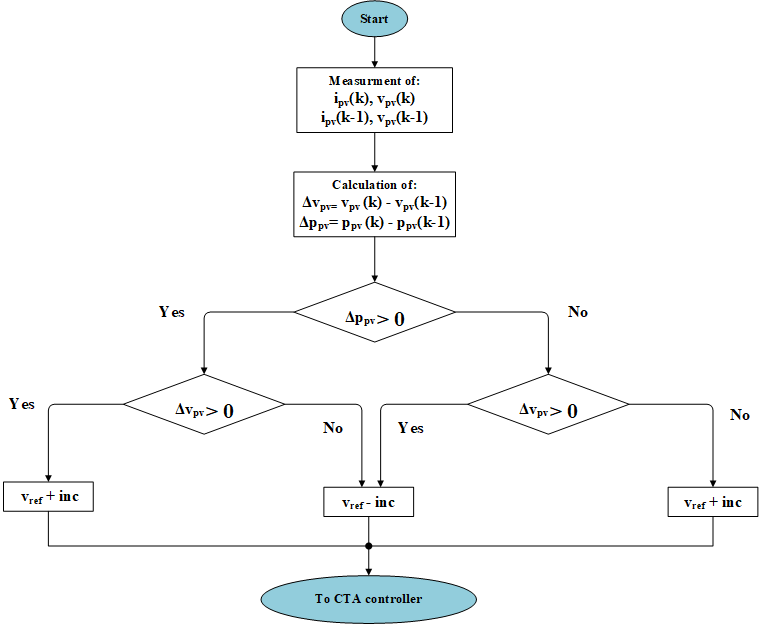
\includegraphics[width=\linewidth]{Flow Chart.png}
    \caption{Flowchart of the P\&O-based voltage MPPT algorithm.}
    \label{fig:po-flowchart}
\end{figure}

\subsection{CTA-Based MPPT Control}

The PV-voltage tracking error and integral sliding variable are
\begin{equation}
e_{pv}=V_{pv}-V_{\mathrm{ref}},
\end{equation}
\begin{equation}
s=\int_0^t e_{pv}(\tau)\,d\tau,\qquad \dot s=e_{pv}.
\end{equation}
The CTA auxiliary state is governed by
\begin{equation}
\dot\eta=-k_3\left\lceil s\right\rfloor^0-k_4\left\lceil\dot s\right\rfloor^0,
\label{eq:cta-eta}
\end{equation}
and the duty-cycle command is
\begin{equation}
D=-k_1\left\lceil s\right\rfloor^{1/3}-k_2\left\lceil\dot s\right\rfloor^{1/2}+\eta.
\label{eq:cta-mppt}
\end{equation}
The implemented duty cycle is constrained to $0\leq D\leq1$.

\subsection{DIC-Based MPPT Control}

Define
\begin{equation}
\sigma_1=s+k_2\left\lceil\dot s\right\rfloor^{3/2},\qquad
\sigma_2=s+k_4\left\lceil\dot s\right\rfloor^{3/2}.
\end{equation}
The DIC law is
\begin{equation}
D=-k_1\left\lceil\sigma_1\right\rfloor^{1/3}+\bar v,
\label{eq:dic-mppt}
\end{equation}
\begin{equation}
\dot{\bar v}=-k_3\left\lceil\sigma_2\right\rfloor^0.
\label{eq:dic-vbar}
\end{equation}

\section{Design of the Utkin Sliding-Mode Observer}
\label{sec:observer}

The observer reconstructs the states required by the inverter controllers using the known inputs and measured grid-side currents. The measured output is
\begin{equation}
y=\begin{bmatrix}I_{gd}&I_{gq}\end{bmatrix}^{T}=Cx,
\end{equation}
where
\begin{equation}
C=\begin{bmatrix}1&0&0&0&0&0\\0&0&0&1&0&0\end{bmatrix}.
\end{equation}
The observability condition is
\begin{equation}
\operatorname{rank}\begin{bmatrix}C^T&(CA)^T&\cdots&(CA^5)^T\end{bmatrix}^{T}=6.
\end{equation}

Let $\hat x$ denote the estimated state and $e_o=y-C\hat x$ the measured-output estimation error. The observer is written in compact form as
\begin{equation}
\dot{\hat x}=A\hat x+Bu+Ge_o+L\nu,
\label{eq:observer-compact}
\end{equation}
where
\begin{equation}
\nu=\begin{bmatrix}M_1\operatorname{sign}(e_{o1})&M_2\operatorname{sign}(e_{o2})\end{bmatrix}^{T}.
\end{equation}
The estimated variables $\hat V_{cd}$, $\hat V_{cq}$, $\hat I_d$, and $\hat I_q$ are supplied to the inverter-control implementation.

\section{Design of the Inverter Controllers}
\label{sec:inverter}

The outer DC-link controller generates $I_{gd}^{*}$, while
\begin{equation}
I_{gq}^{*}=0
\end{equation}
is selected to limit reactive-power exchange. The current errors are
\begin{equation}
e_d=I_{gd}-I_{gd}^{*},\qquad e_q=I_{gq}-I_{gq}^{*}.
\end{equation}
The proportional--integral sliding variables are
\begin{equation}
S_d=e_d+Z_d\int_0^t e_d(\tau)\,d\tau,
\end{equation}
\begin{equation}
S_q=e_q+Z_q\int_0^t e_q(\tau)\,d\tau,
\end{equation}
where $Z_d>0$ and $Z_q>0$.

\begin{figure}[htbp]
    \centering
    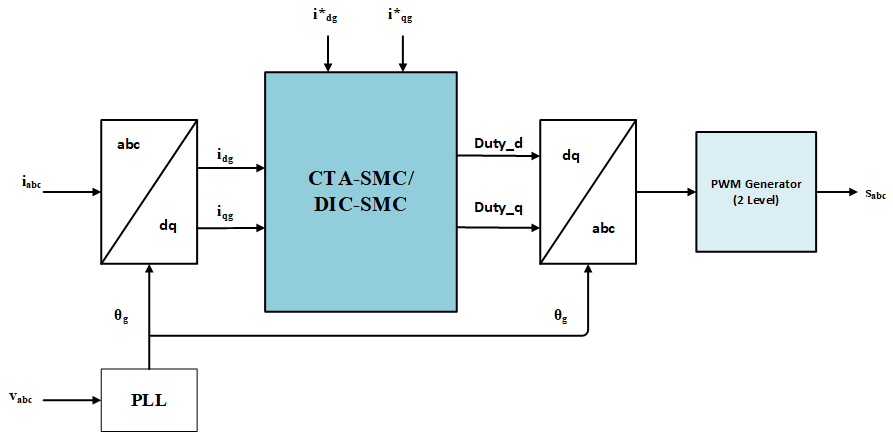
\includegraphics[width=\linewidth]{CTA-SMC Invervter.png}
    \caption{CTA-based inverter current-control structure.}
    \label{fig:cta-inverter}
\end{figure}

\subsection{CTA-Based Inverter Control}

The auxiliary dynamics are
\begin{equation}
\dot\eta_d=-k_{3d}\left\lceil S_d\right\rfloor^0-k_{4d}\left\lceil\dot S_d\right\rfloor^0,
\end{equation}
\begin{equation}
\dot\eta_q=-k_{3q}\left\lceil S_q\right\rfloor^0-k_{4q}\left\lceil\dot S_q\right\rfloor^0.
\end{equation}
The control commands are
\begin{equation}
D_d=-k_{1d}\left\lceil S_d\right\rfloor^{1/3}-k_{2d}\left\lceil\dot S_d\right\rfloor^{1/2}+\eta_d,
\end{equation}
\begin{equation}
D_q=-k_{1q}\left\lceil S_q\right\rfloor^{1/3}-k_{2q}\left\lceil\dot S_q\right\rfloor^{1/2}+\eta_q.
\end{equation}

\subsection{DIC-Based Inverter Control}

For $j\in\{d,q\}$, define
\begin{equation}
\sigma_{1j}=S_j+k_{2j}\left\lceil\dot S_j\right\rfloor^{3/2},\qquad
\sigma_{2j}=S_j+k_{4j}\left\lceil\dot S_j\right\rfloor^{3/2}.
\end{equation}
The DIC commands are
\begin{equation}
D_j=-k_{1j}\left\lceil\sigma_{1j}\right\rfloor^{1/3}+\bar v_j,
\end{equation}
\begin{equation}
\dot{\bar v}_j=-k_{3j}\left\lceil\sigma_{2j}\right\rfloor^0.
\end{equation}
The $dq$ commands are transformed to the three-phase frame and implemented using the selected PWM method.

\section{Stability Analysis}
\label{sec:stability}

The analysis assumes that the lumped matched disturbance in each controlled channel has a bounded derivative, the control-effectiveness gain has a known constant sign and is bounded away from zero, and the CTA and DIC gains satisfy the sufficient conditions in \cite{torres2017design,moreno2017discontinuous}.

For the MPPT loop, let $x_1=s$ and $x_2=\dot s=e_{pv}$. Under the stated assumptions, the CTA closed loop has the canonical form
\begin{equation}
\begin{aligned}
\dot x_1&=x_2,\\
\dot x_2&=-k_1\left\lceil x_1\right\rfloor^{1/3}-k_2\left\lceil x_2\right\rfloor^{1/2}+\eta+\varphi(t),\\
\dot\eta&=-k_3\left\lceil x_1\right\rfloor^0-k_4\left\lceil x_2\right\rfloor^0.
\end{aligned}
\end{equation}
The CTA finite-time convergence result in \cite{torres2017design} implies $s\to0$ and $e_{pv}\to0$ in finite time. Hence, $V_{pv}$ converges to the reference generated by the P\&O algorithm.

For the DIC loop, simultaneous convergence of $\sigma_1$ and $\sigma_2$ to zero, with $k_2\neq k_4$, implies $x_2=0$ and subsequently $x_1=0$. The corresponding finite-time result follows from \cite{moreno2017discontinuous} under the stated gain and disturbance conditions.

For the inverter loops, finite-time convergence of $S_d$ and $S_q$ to their sliding manifolds yields
\begin{equation}
\dot e_d+Z_de_d=0,\qquad \dot e_q+Z_qe_q=0.
\end{equation}
Therefore, after the reaching times $T_d$ and $T_q$,
\begin{equation}
e_d(t)=e_d(T_d)e^{-Z_d(t-T_d)},\qquad e_q(t)=e_q(T_q)e^{-Z_q(t-T_q)},
\end{equation}
which establishes exponential convergence for $Z_d,Z_q>0$. These conclusions apply to the individual controlled channels; the complete interconnected behavior is evaluated numerically.

\section{Simulation Results and Discussion}
\label{sec:results}

The controllers were implemented in MATLAB/Simulink and evaluated under time-varying irradiance while the PV-cell temperature was maintained at $25\,^{\circ}\mathrm{C}$. The DC-link reference was $V_{dc}^{*}=750~\mathrm{V}$, and $I_{gq}^{*}=0$.

\begin{table}[htbp]
\centering
\caption{PV-module and grid parameters.}
\label{tab:system-params}
\begin{tabular}{lc}
\toprule
Parameter & Value\\
\midrule
PV-module peak power & $213~\mathrm{W}$\\
Voltage at maximum power & $29~\mathrm{V}$\\
Current at maximum power & $7.35~\mathrm{A}$\\
Short-circuit current & $7.84~\mathrm{A}$\\
Open-circuit voltage & $36.3~\mathrm{V}$\\
Temperature coefficient of $I_{sc}$ & $0.102~\%/^{\circ}\mathrm{C}$\\
Temperature coefficient of $V_{oc}$ & $-0.361~\%/^{\circ}\mathrm{C}$\\
Grid line-to-line RMS voltage & $380~\mathrm{V}$\\
Grid frequency & $50~\mathrm{Hz}$\\
DC-link reference voltage & $750~\mathrm{V}$\\
\bottomrule
\end{tabular}
\end{table}

\begin{table}[htbp]
\centering
\caption{LCL-filter parameters.}
\label{tab:lcl-params}
\begin{tabular}{lc}
\toprule
Parameter & Value\\
\midrule
Inverter-side inductance $L_i$ & $0.91~\mathrm{mH}$\\
Filter capacitance $C_f$ & $0.5~\mathrm{mF}$\\
Grid-side inductance $L_g$ & $5.5~\mathrm{mH}$\\
Damping resistance $R_d$ & $0.3~\Omega$\\
\bottomrule
\end{tabular}
\end{table}

\subsection{Irradiance Profile}

\begin{figure}[htbp]
    \centering
    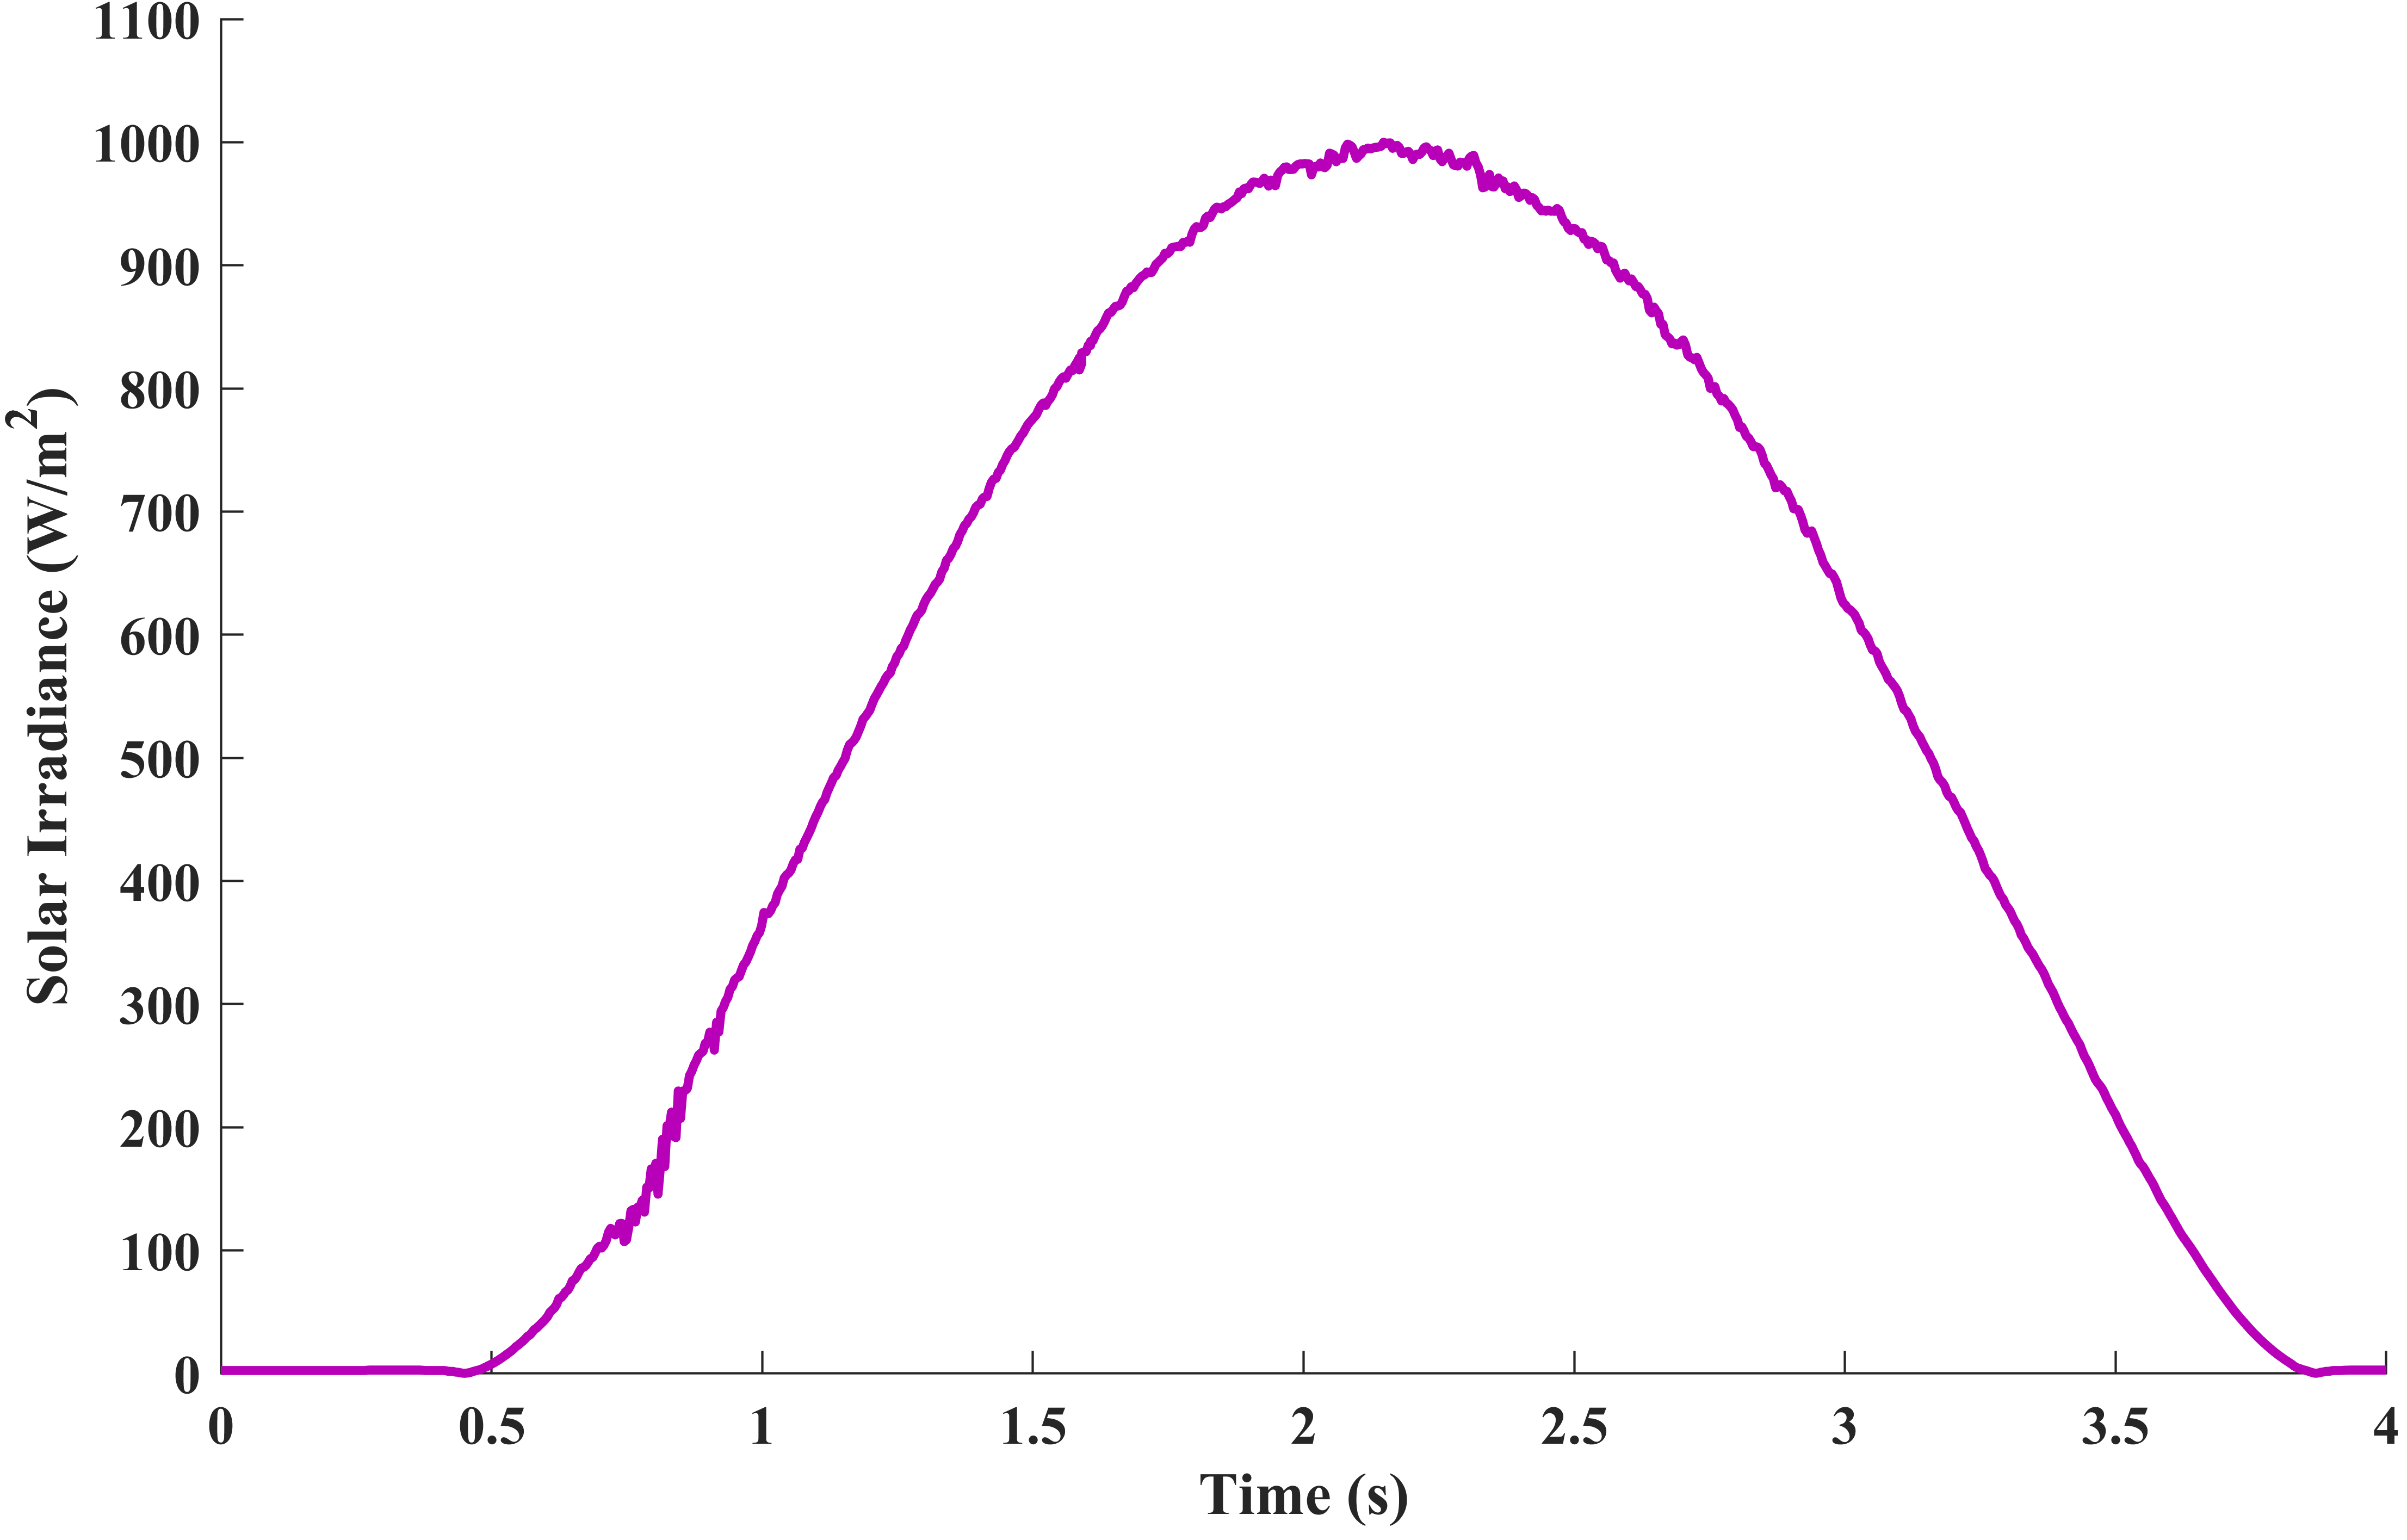
\includegraphics[width=0.9\columnwidth]{Pictures/SOLAR IRREDIANCE.png}
    \caption{Solar-irradiance profile used in the simulations.}
    \label{fig:irradiance}
\end{figure}

The profile contains multiple irradiance levels and transitions to assess the dynamic response of the MPPT and inverter-control loops.

\subsection{Sliding Variables}

\begin{figure}[htbp]
\centering
\begin{subfigure}{0.45\textwidth}
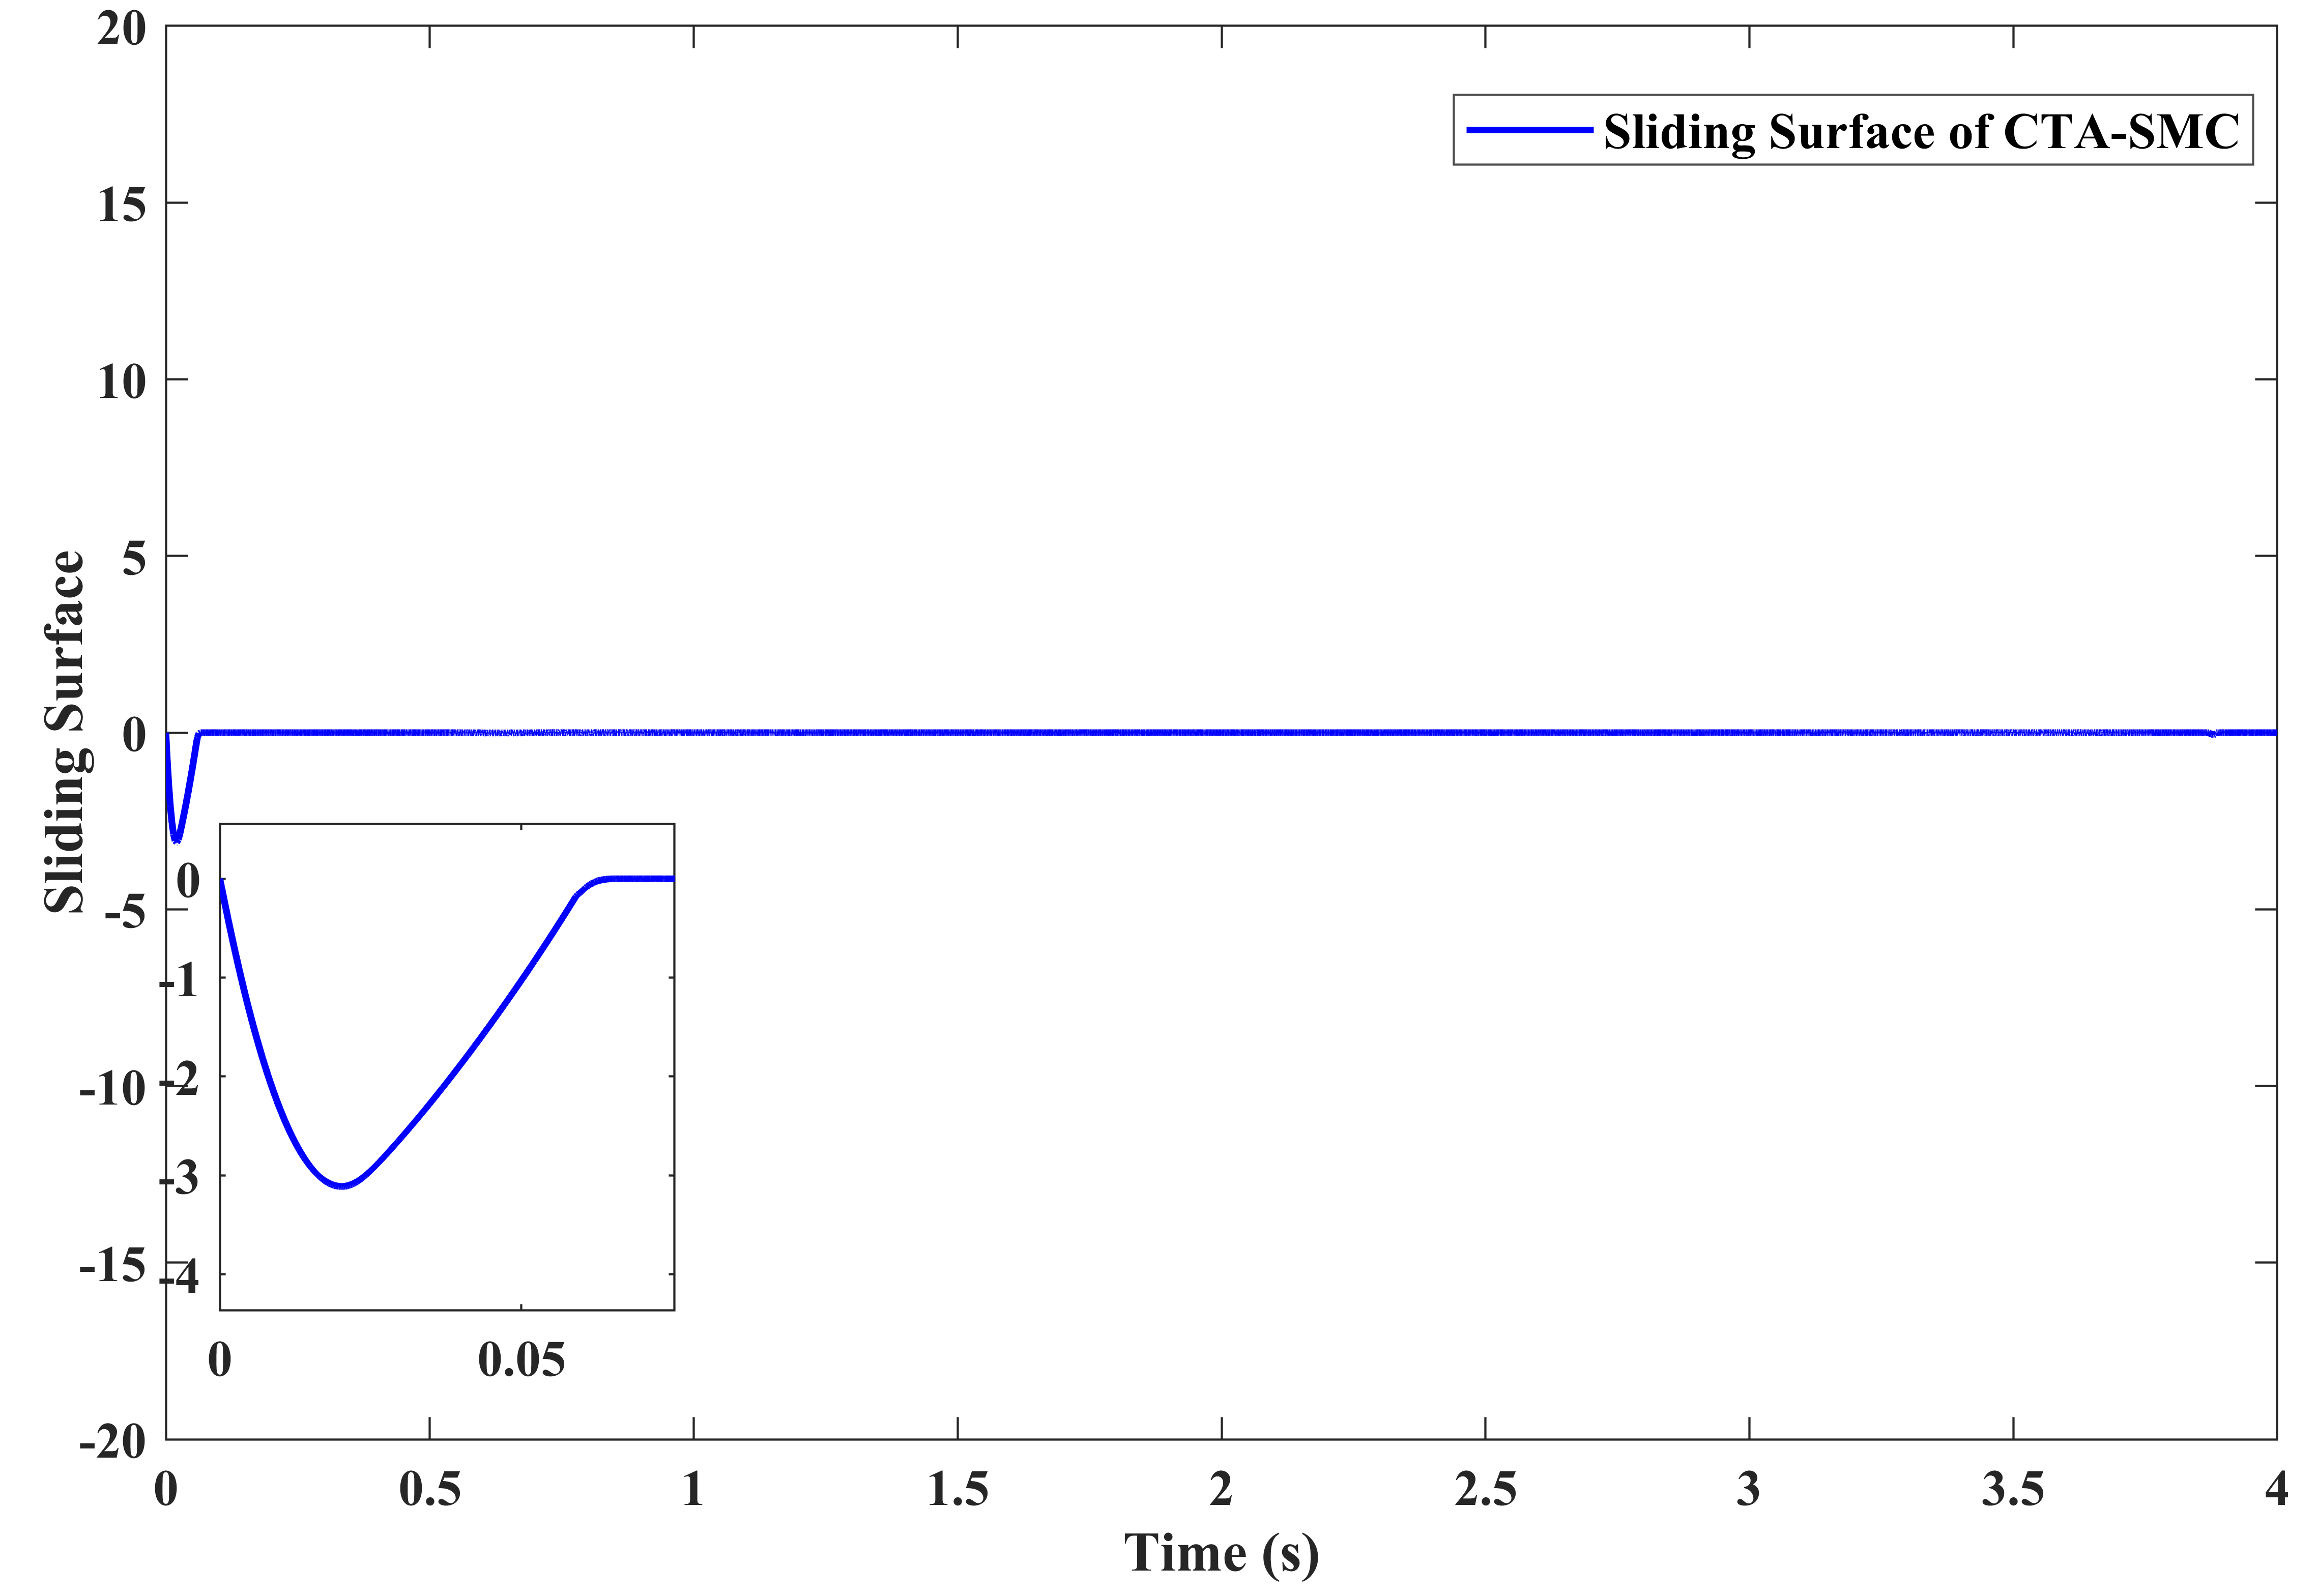
\includegraphics[width=\textwidth,height=4cm,keepaspectratio]{Pictures/CTA Sliding Surface MPPT.png}
\caption{CTA--MPPT.}
\end{subfigure}\hfill
\begin{subfigure}{0.45\textwidth}
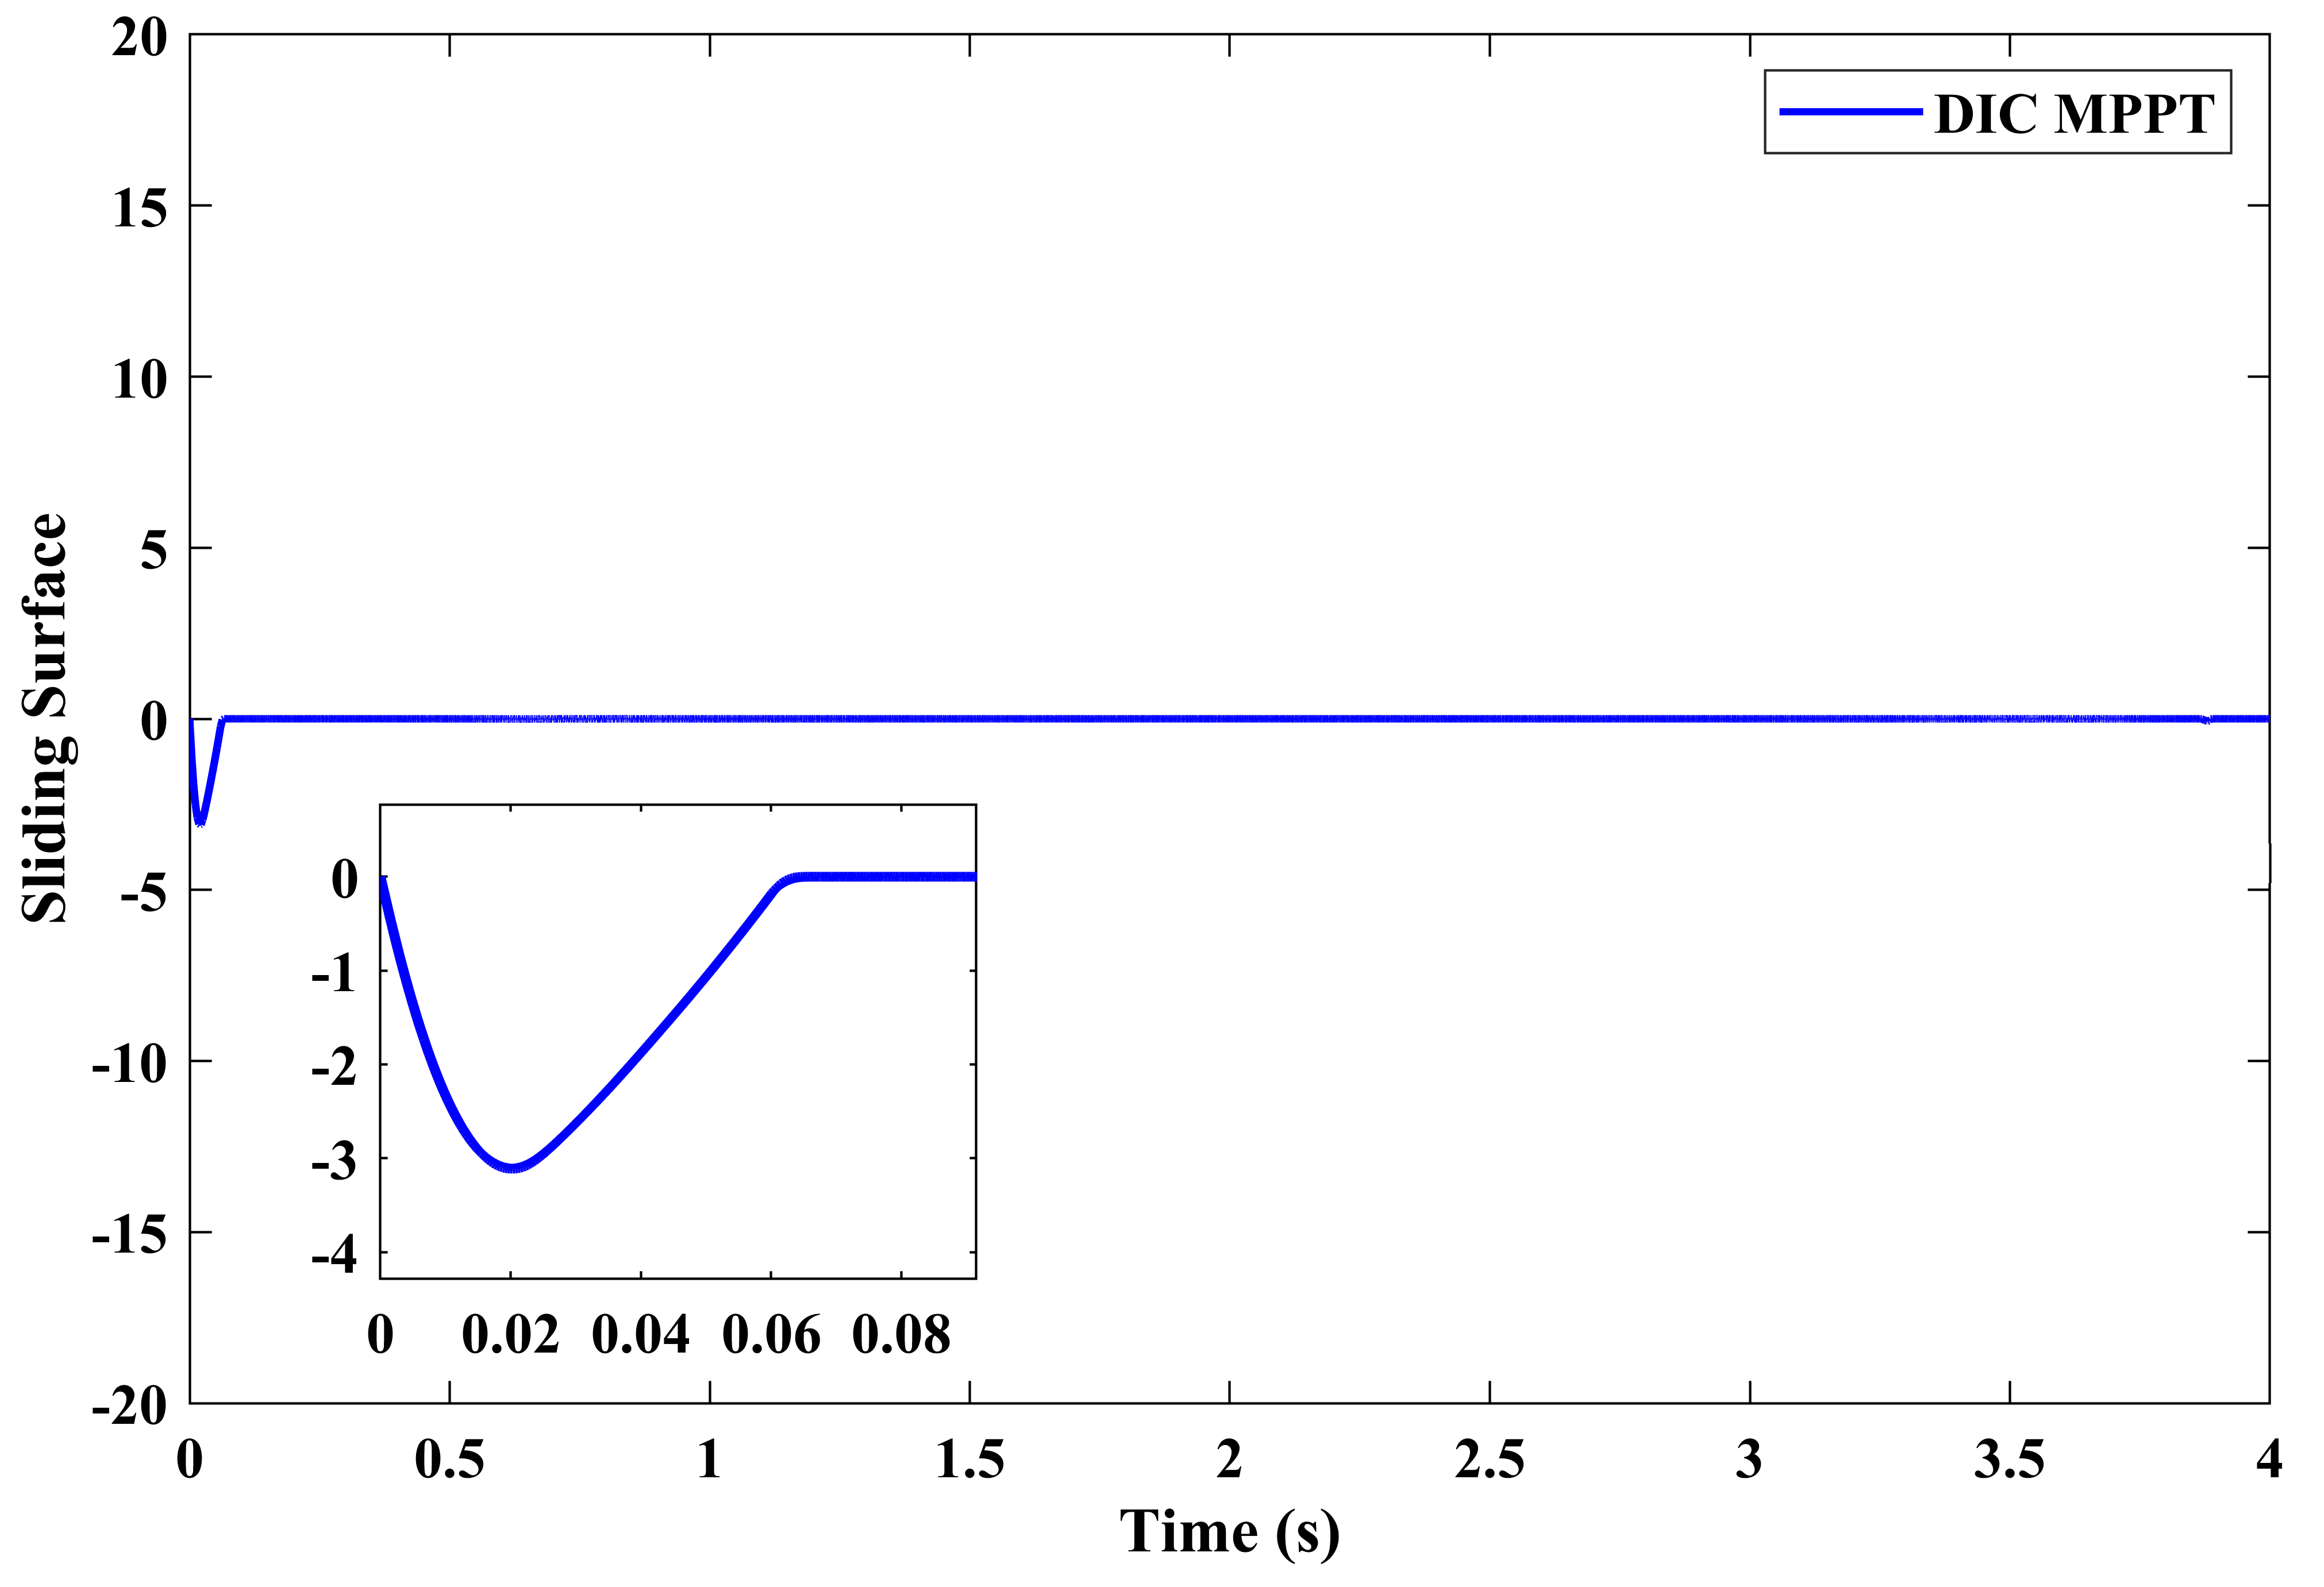
\includegraphics[width=\textwidth,height=4cm,keepaspectratio]{Pictures/Sliding surface DIC mppt.png}
\caption{DIC--MPPT.}
\end{subfigure}
\begin{subfigure}{0.45\textwidth}
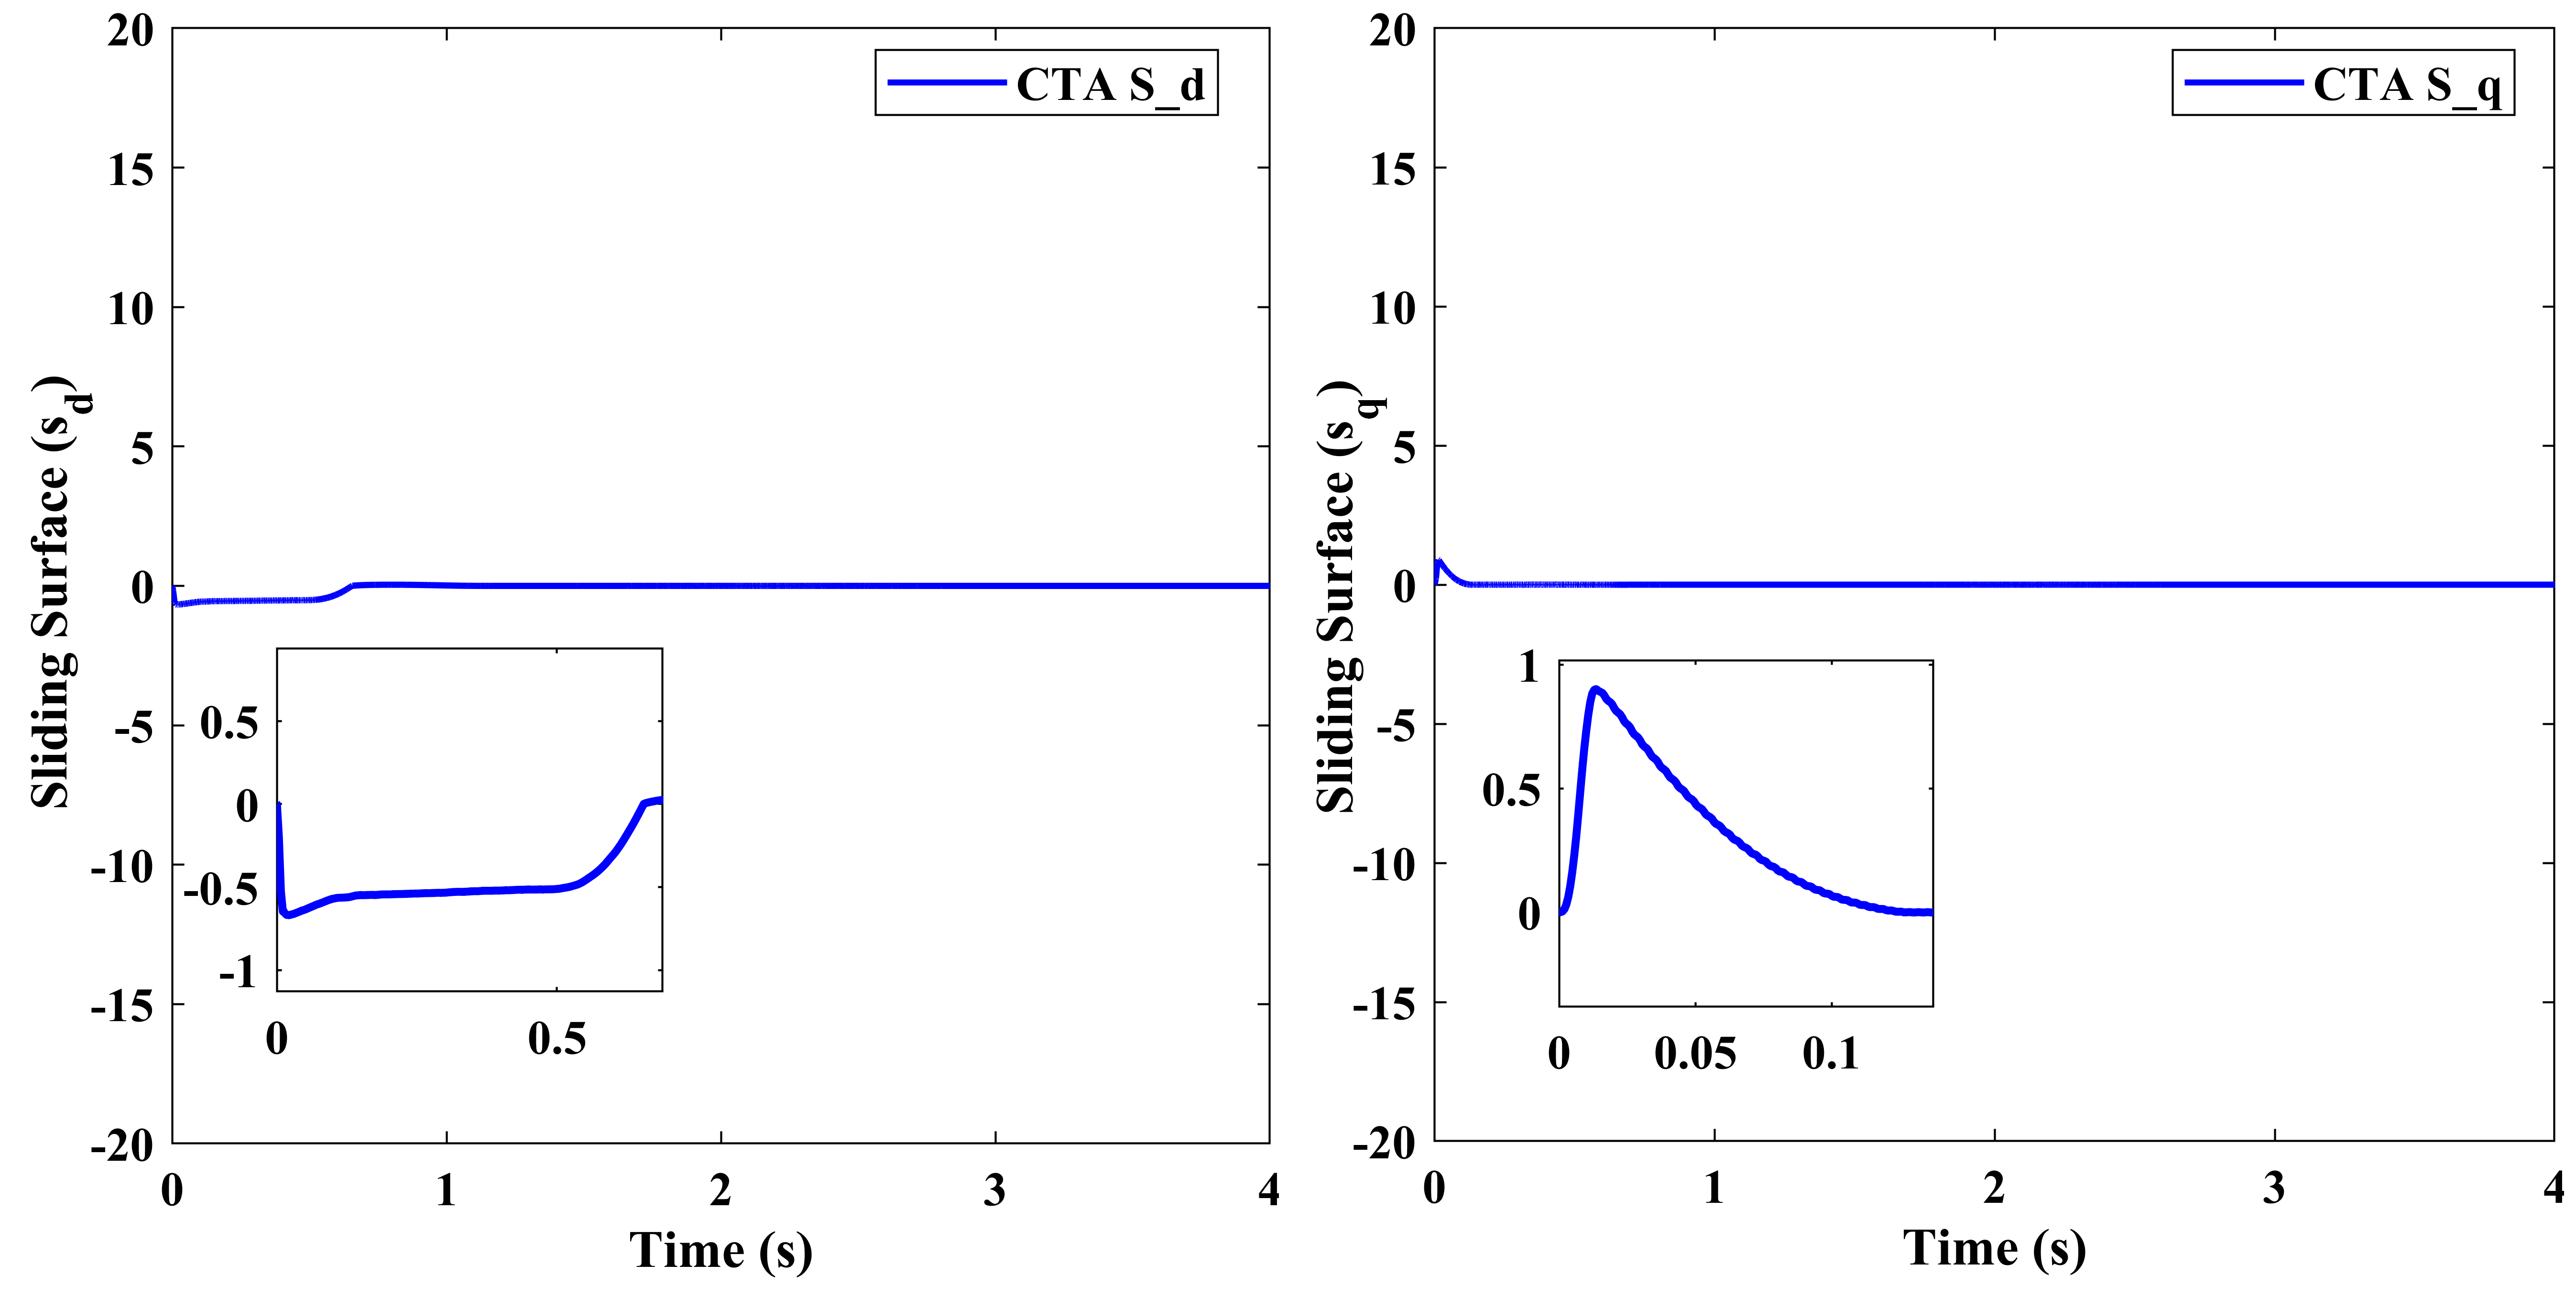
\includegraphics[width=\textwidth,height=4cm,keepaspectratio]{Pictures/Sliding Surface CTA Inverter.png}
\caption{CTA--inverter.}
\end{subfigure}\hfill
\begin{subfigure}{0.45\textwidth}
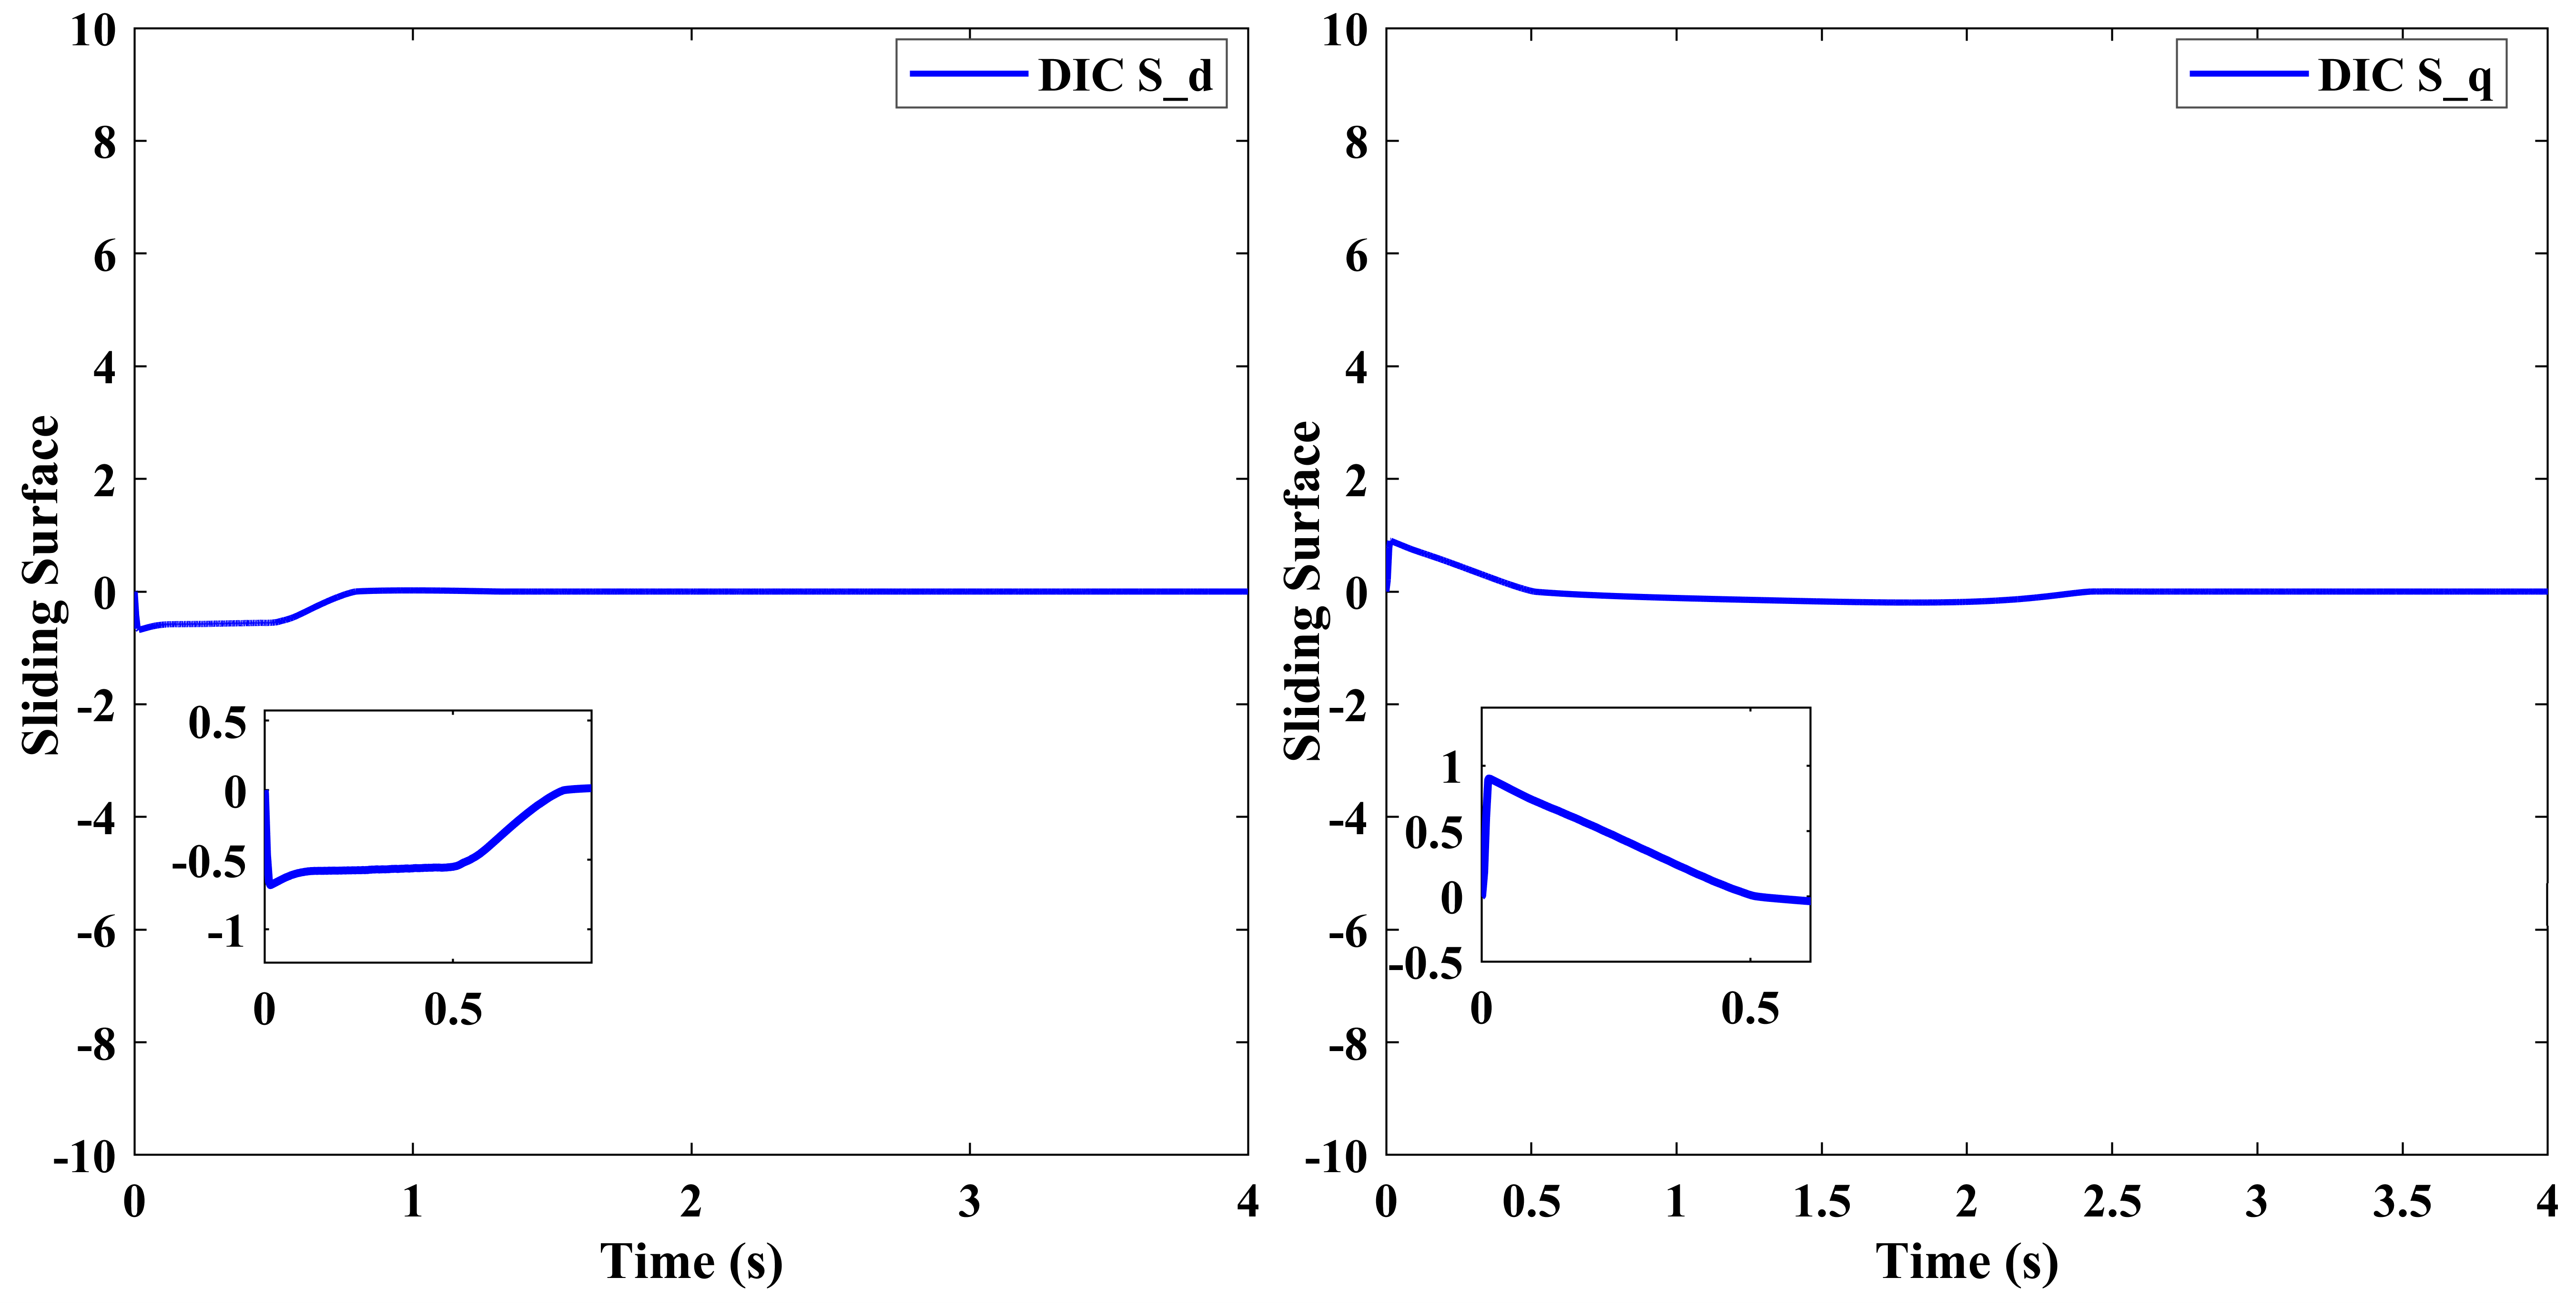
\includegraphics[width=\textwidth,height=4cm,keepaspectratio]{Pictures/Sliding Surface DIC Inverter.png}
\caption{DIC--inverter.}
\end{subfigure}
\caption{Sliding-variable responses of the proposed controllers.}
\label{fig:sliding-surfaces}
\end{figure}

Both controllers drive the MPPT and inverter sliding variables toward their respective manifolds under the tested irradiance conditions.

\subsection{Observer Performance}

\begin{figure}[htbp]
\centering
\begin{subfigure}{0.45\textwidth}
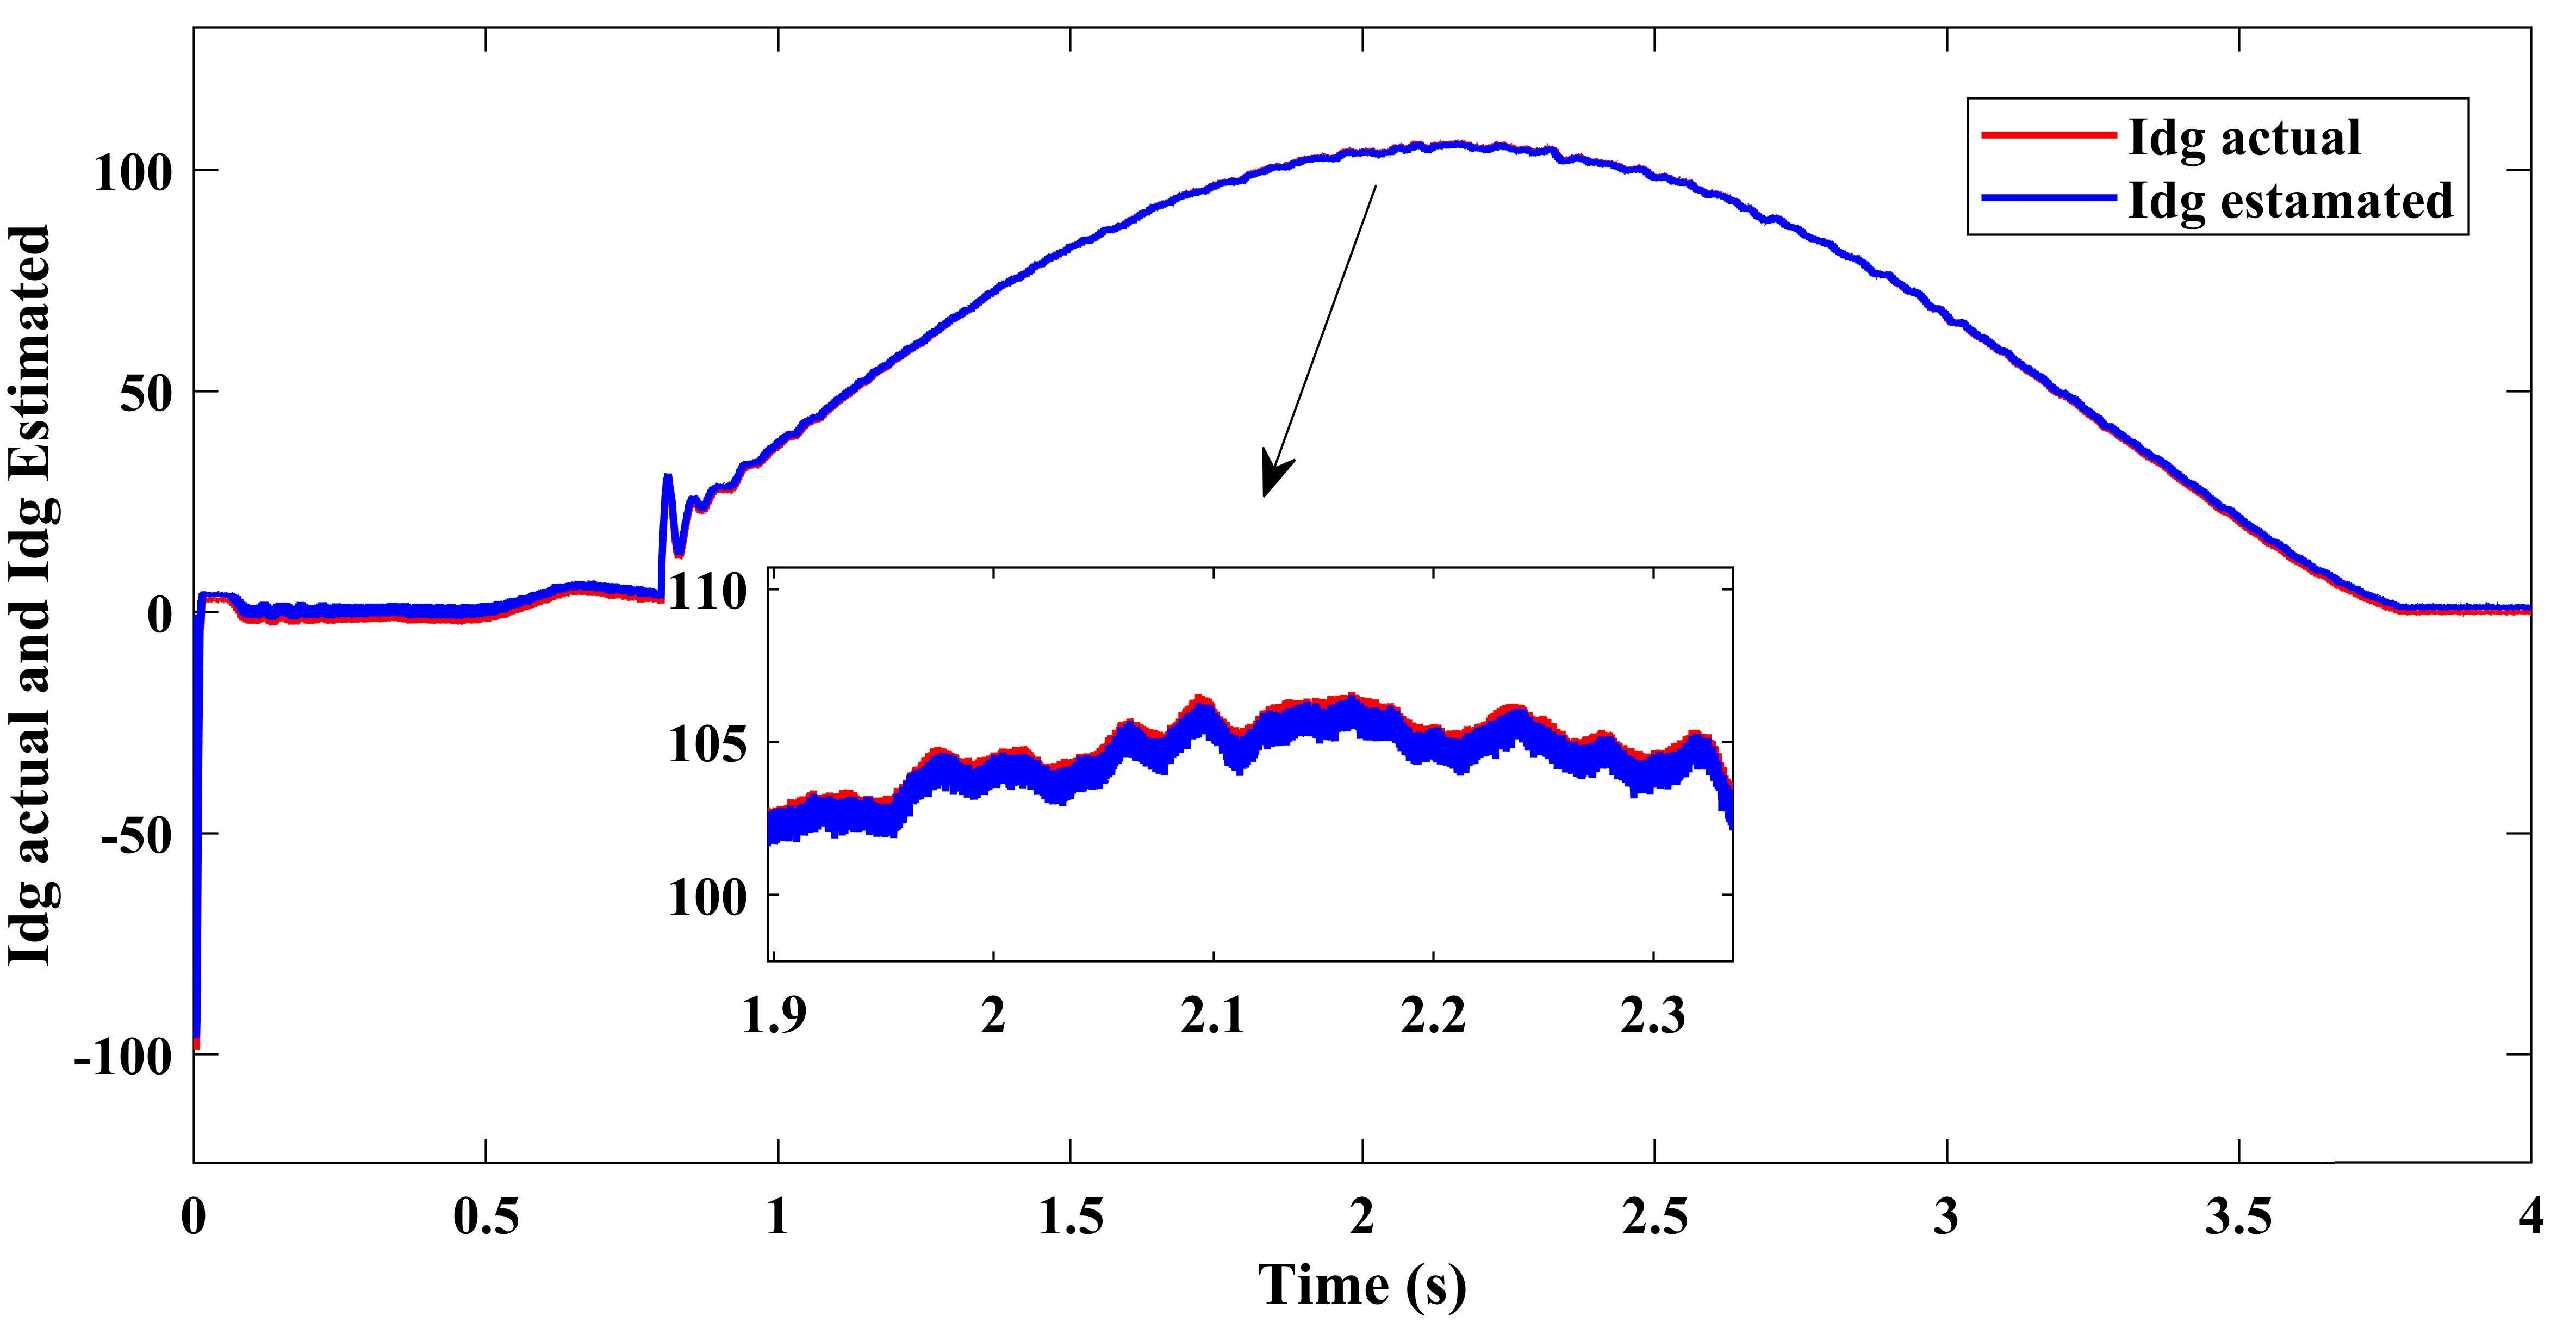
\includegraphics[width=\textwidth,height=4cm,keepaspectratio]{Pictures/Igd Observed.jpg}
\caption{$I_{gd}$.}
\end{subfigure}\hfill
\begin{subfigure}{0.45\textwidth}
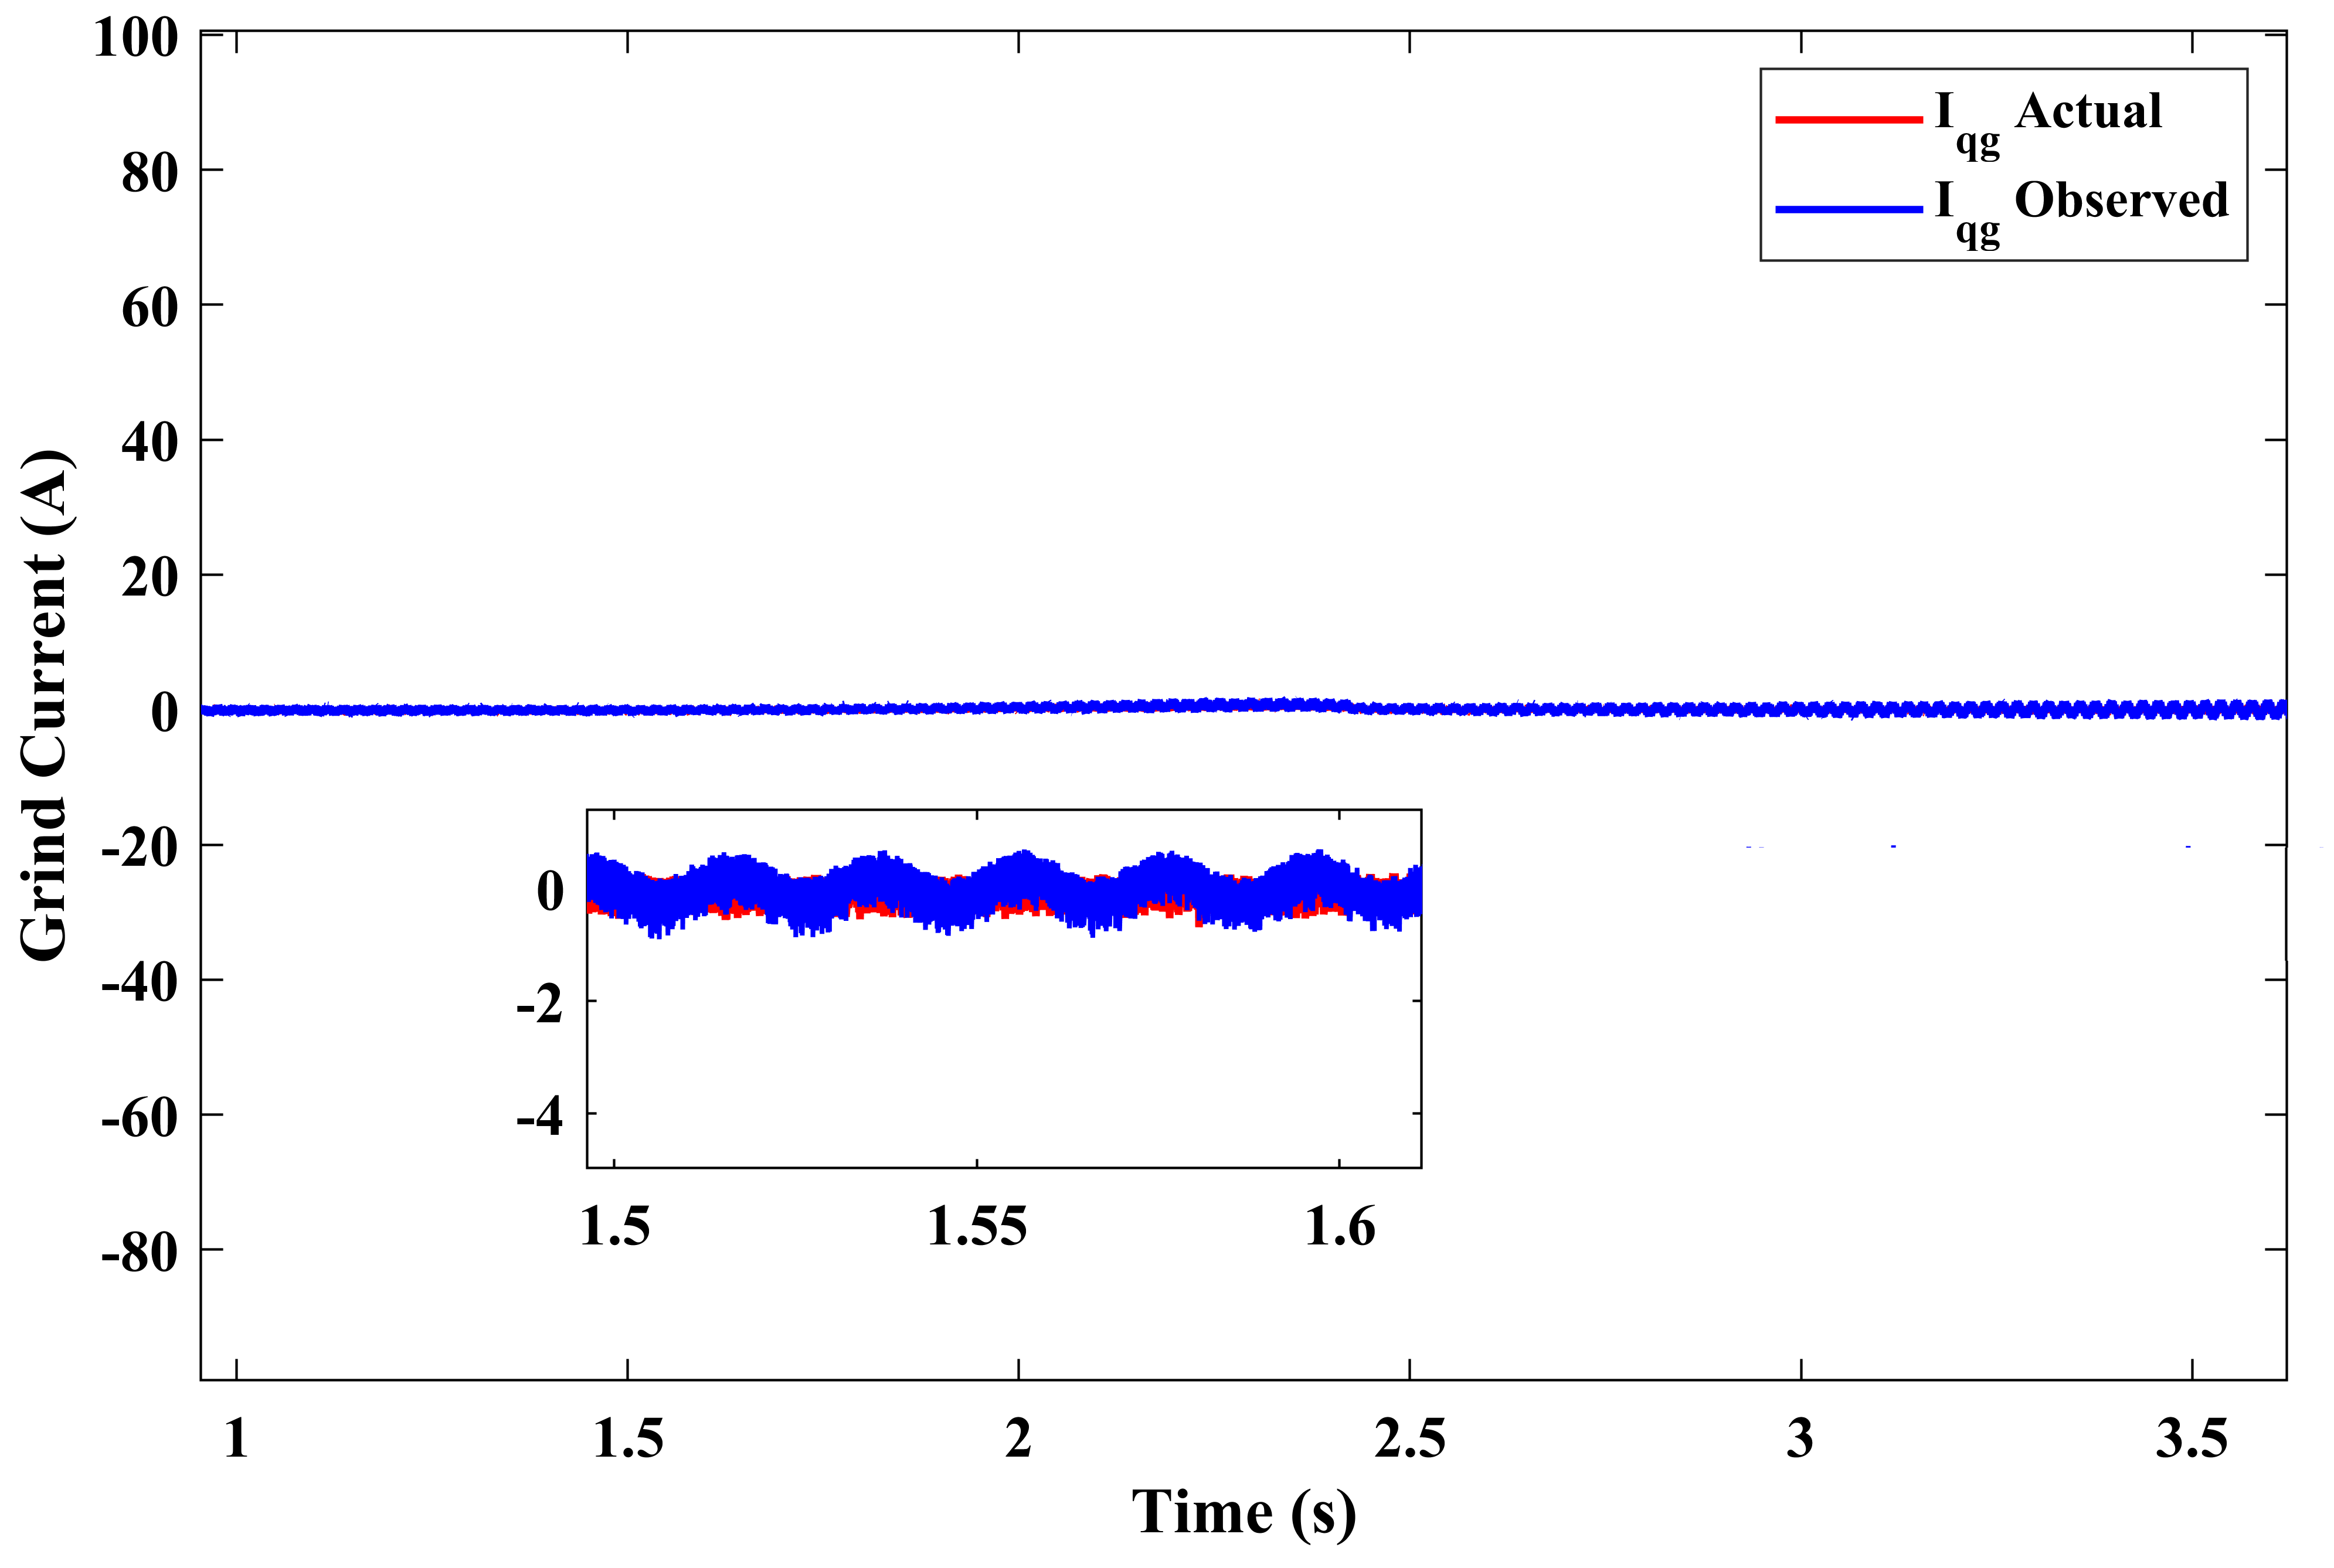
\includegraphics[width=\textwidth,height=4cm,keepaspectratio]{Pictures/Igq Observed.png}
\caption{$I_{gq}$.}
\end{subfigure}
\begin{subfigure}{0.45\textwidth}
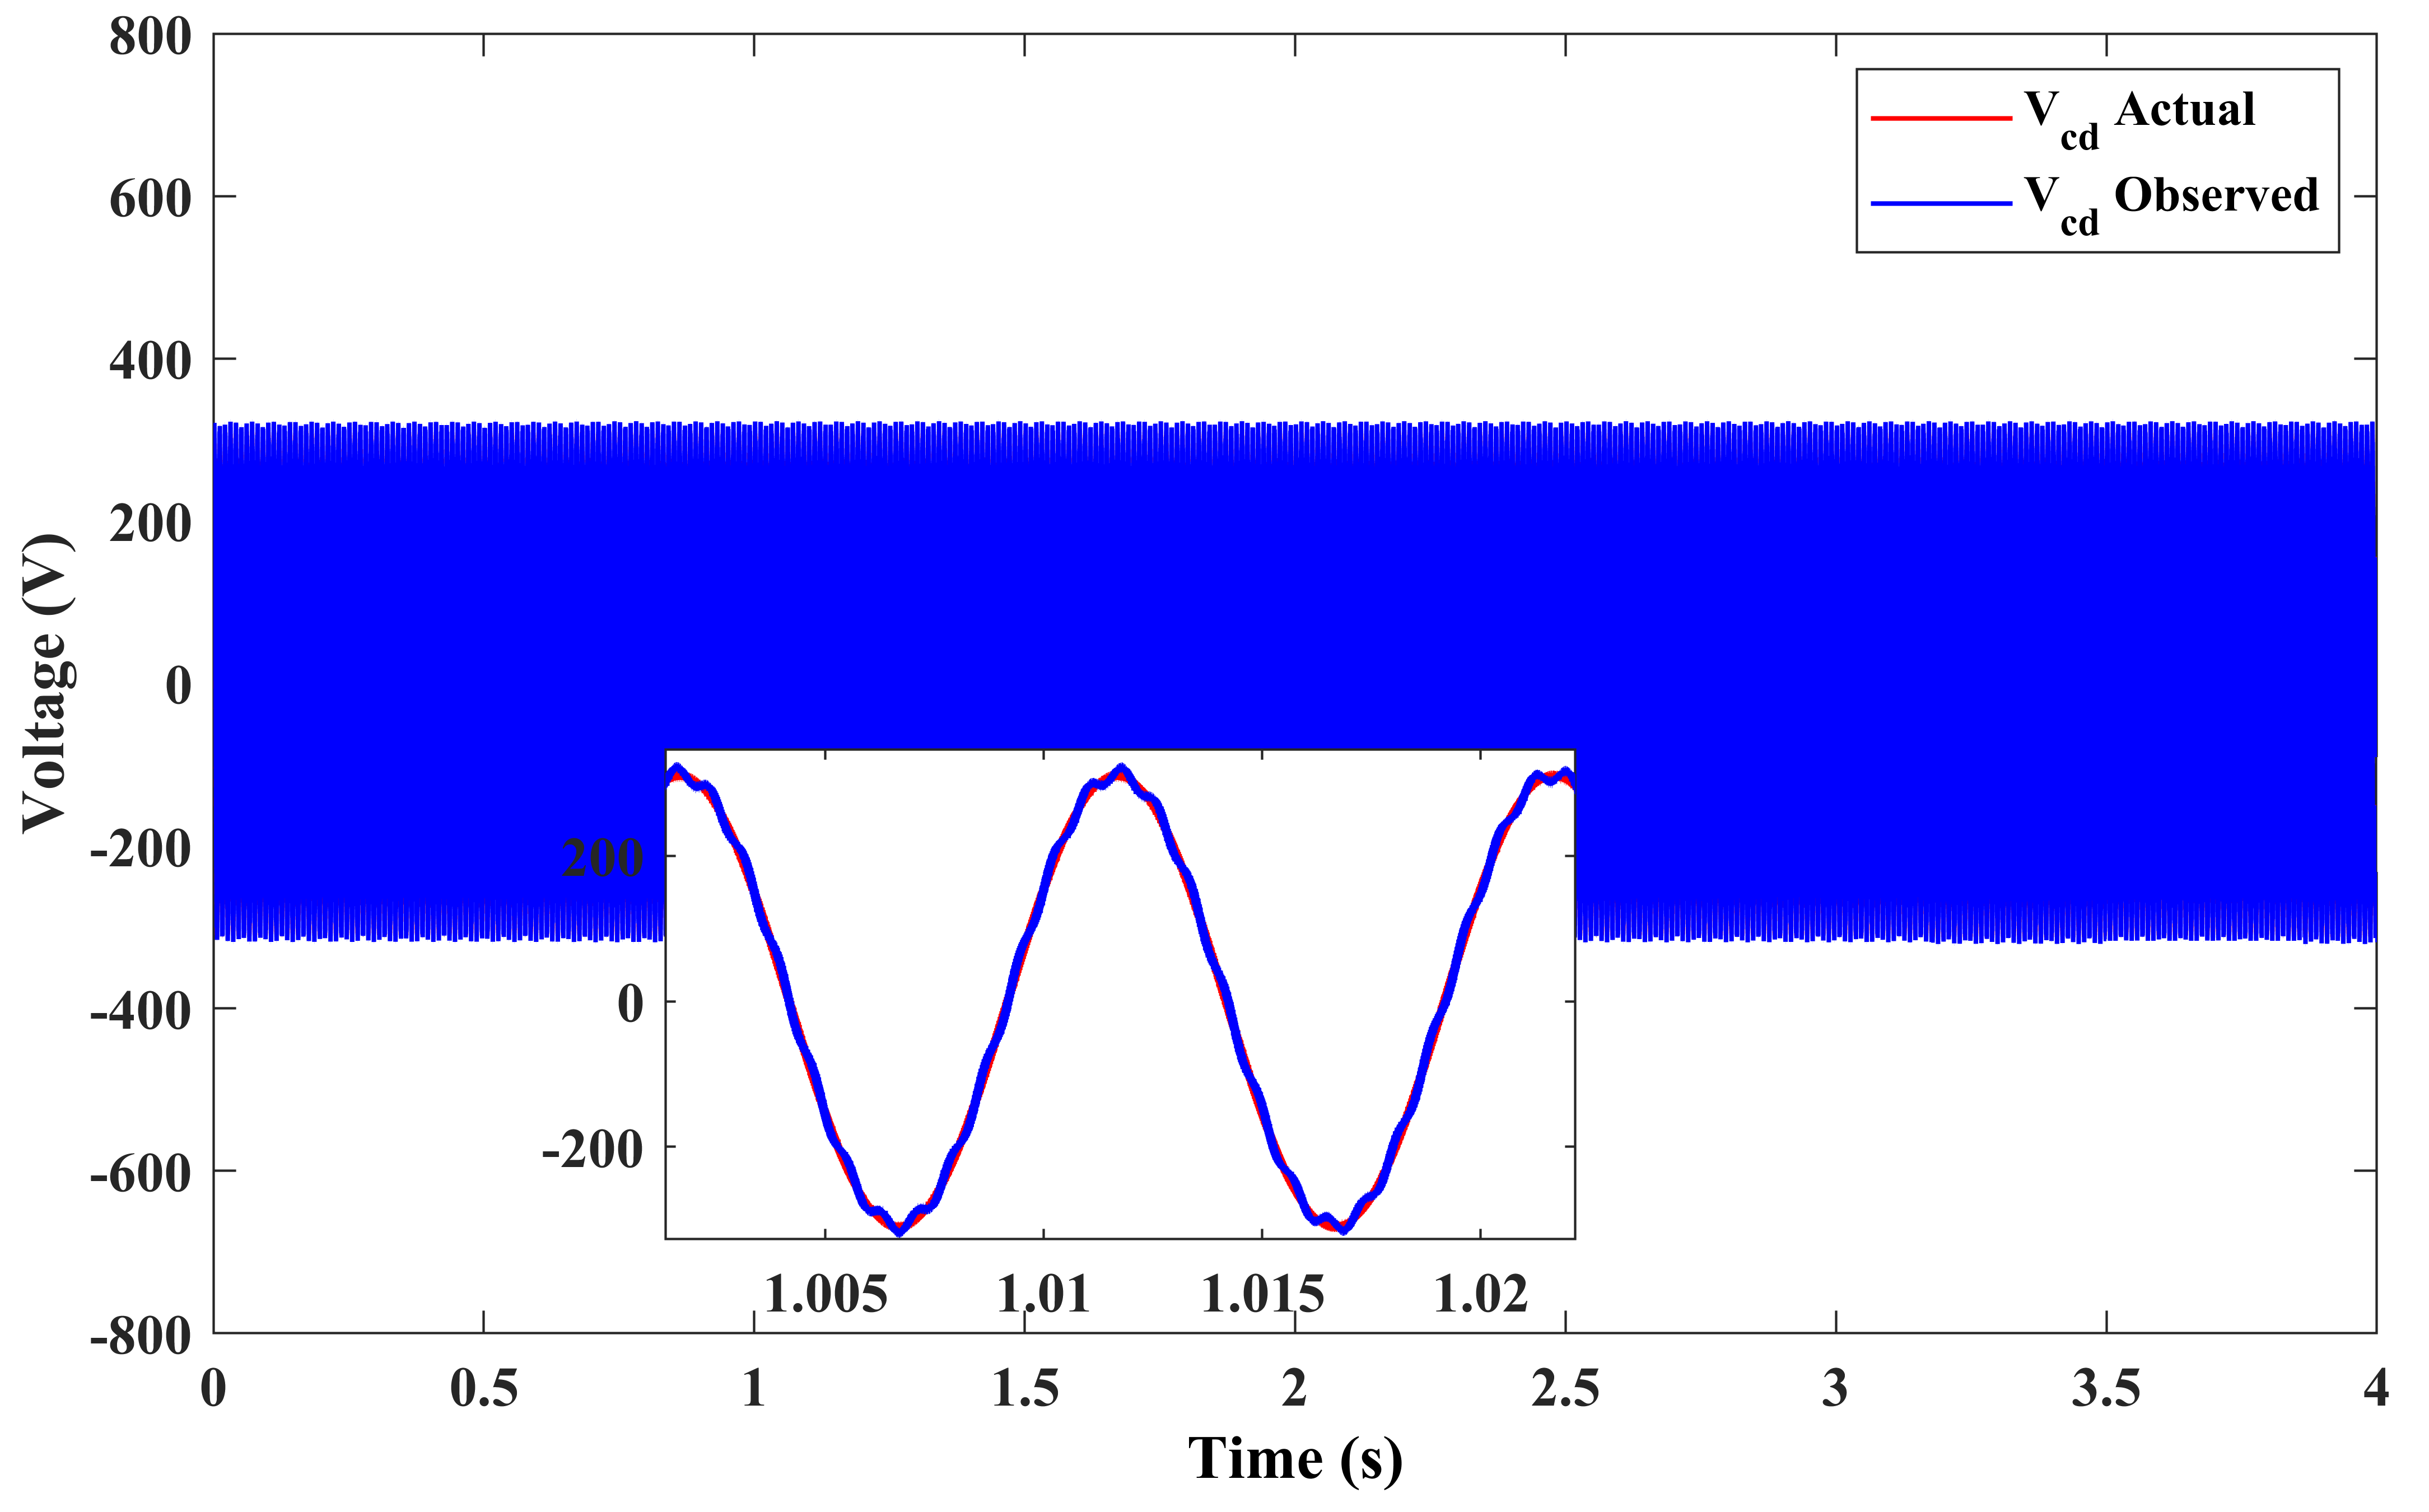
\includegraphics[width=\textwidth,height=4cm,keepaspectratio]{Pictures/Vcd Observed New1.png}
\caption{$V_{cd}$.}
\end{subfigure}\hfill
\begin{subfigure}{0.45\textwidth}
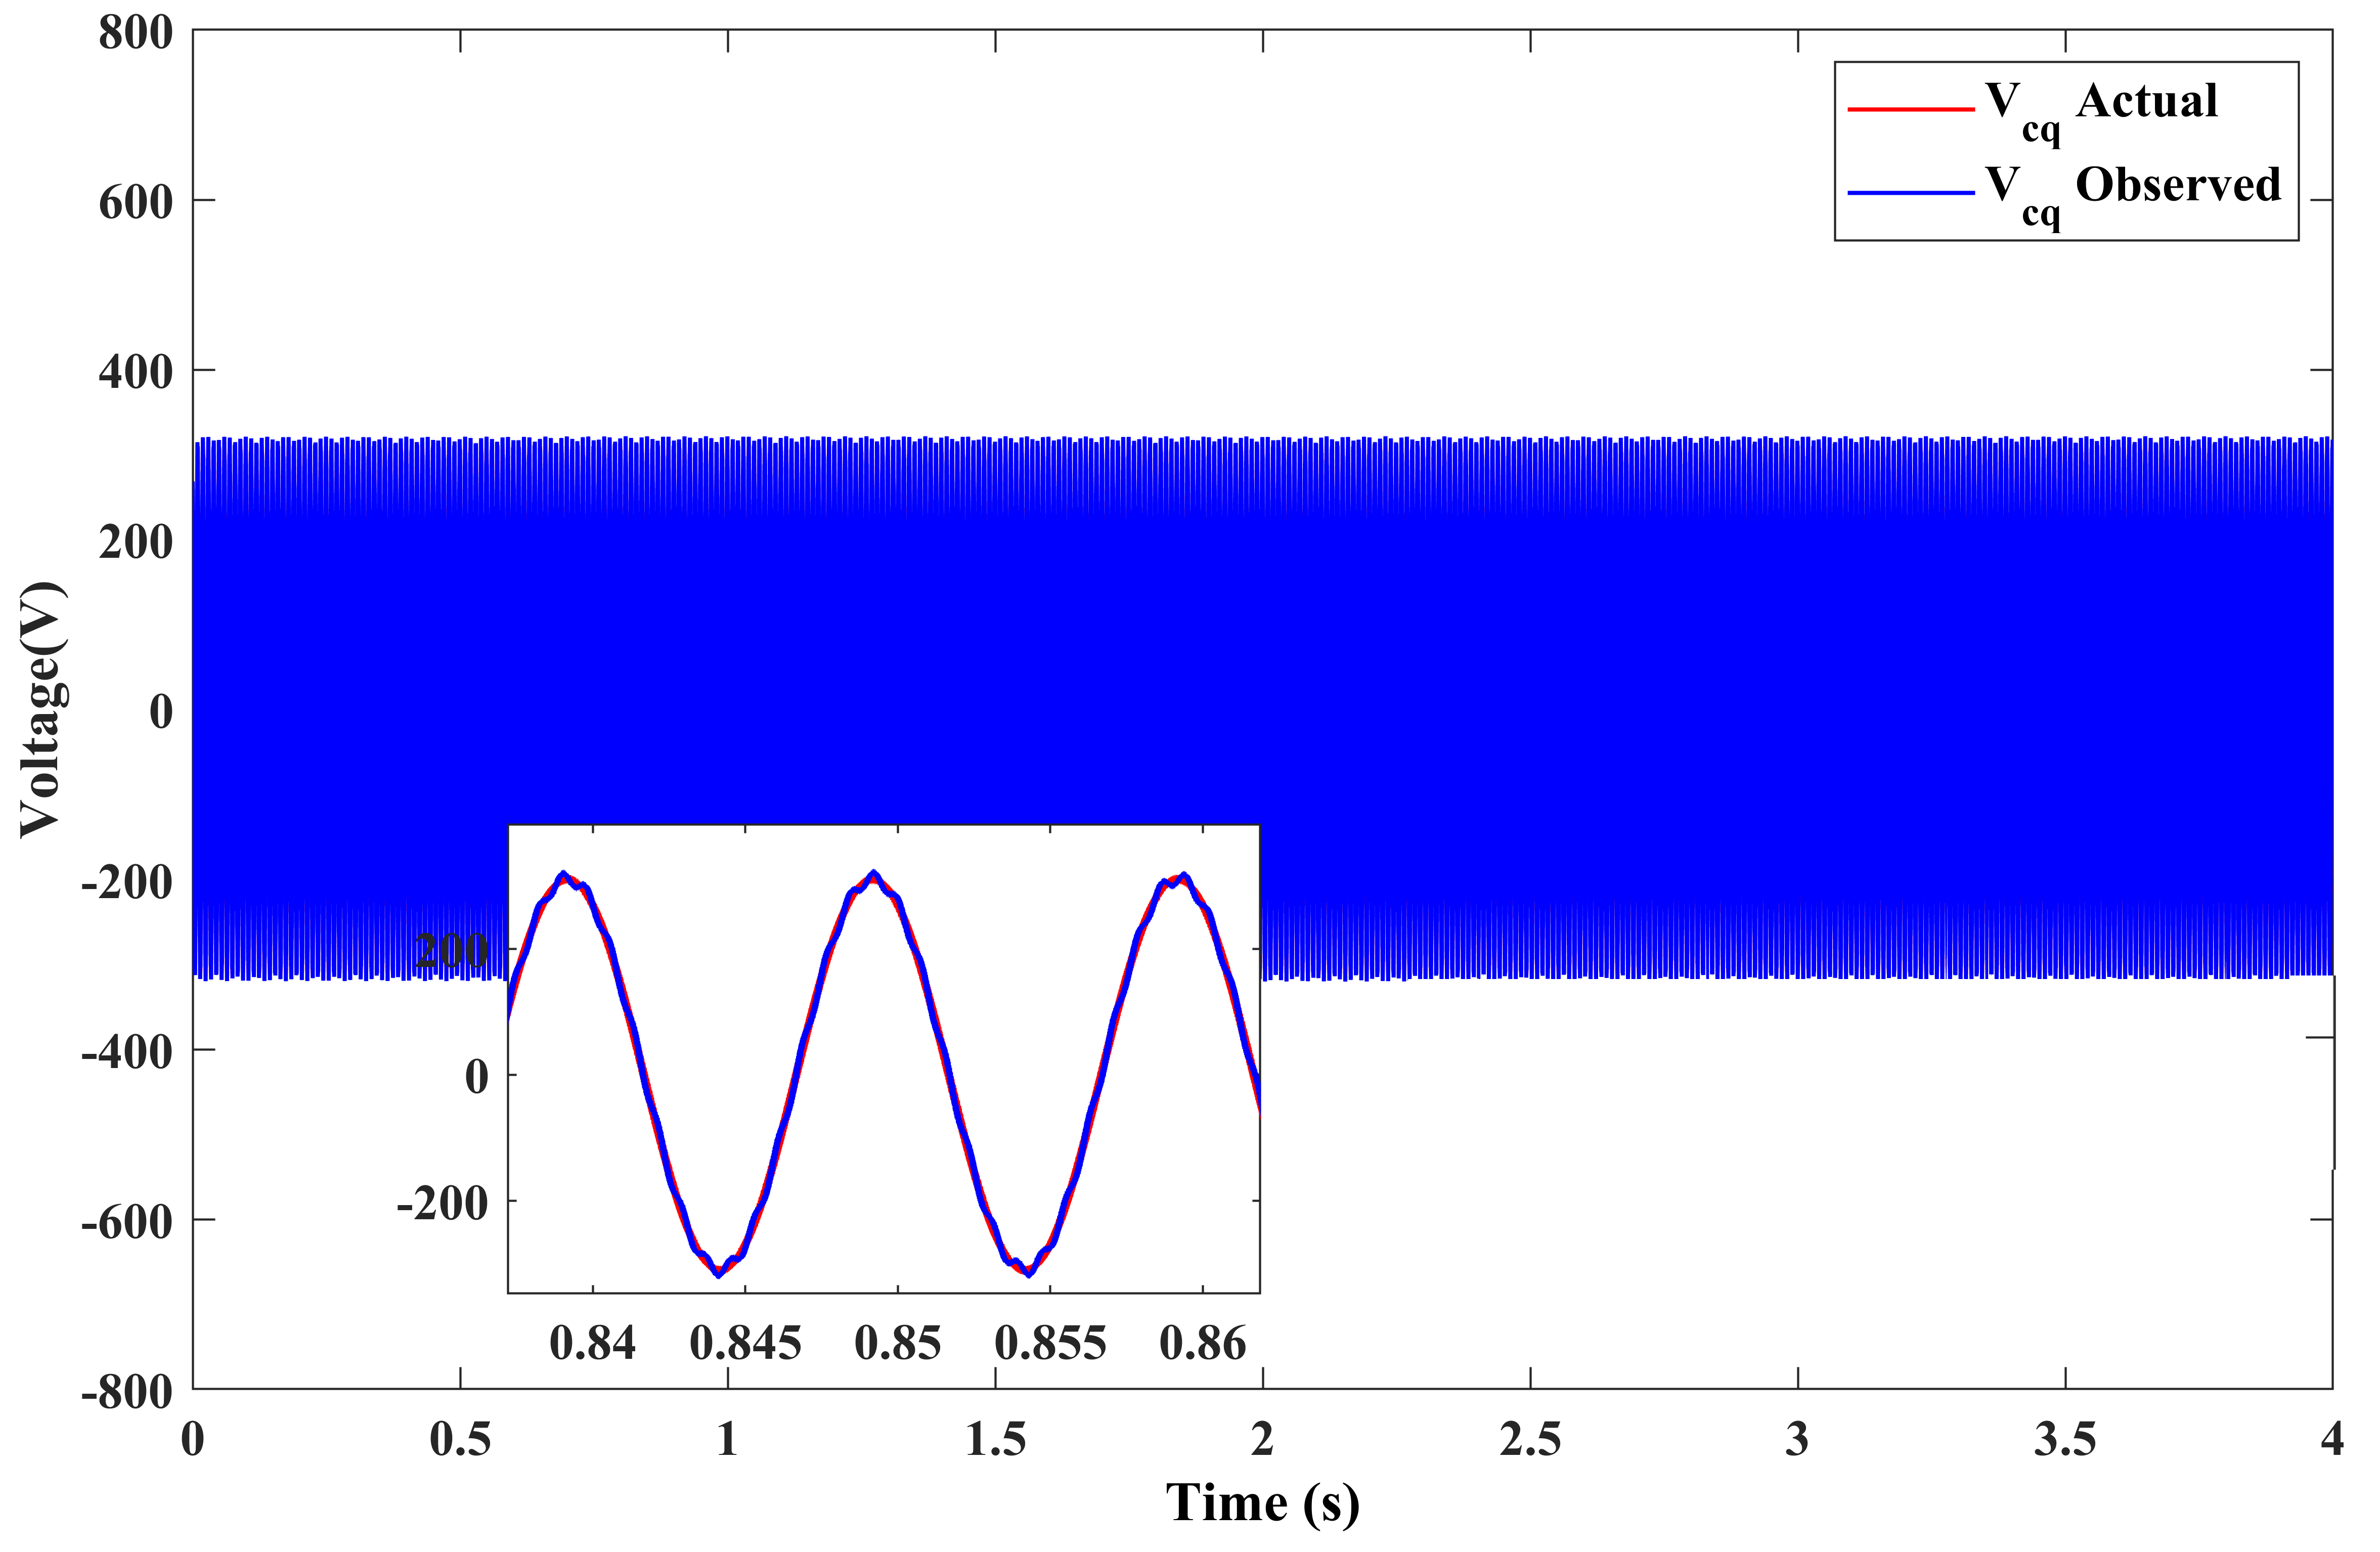
\includegraphics[width=\textwidth,height=4cm,keepaspectratio]{Pictures/Vcq Observed new1.png}
\caption{$V_{cq}$.}
\end{subfigure}
\begin{subfigure}{0.45\textwidth}
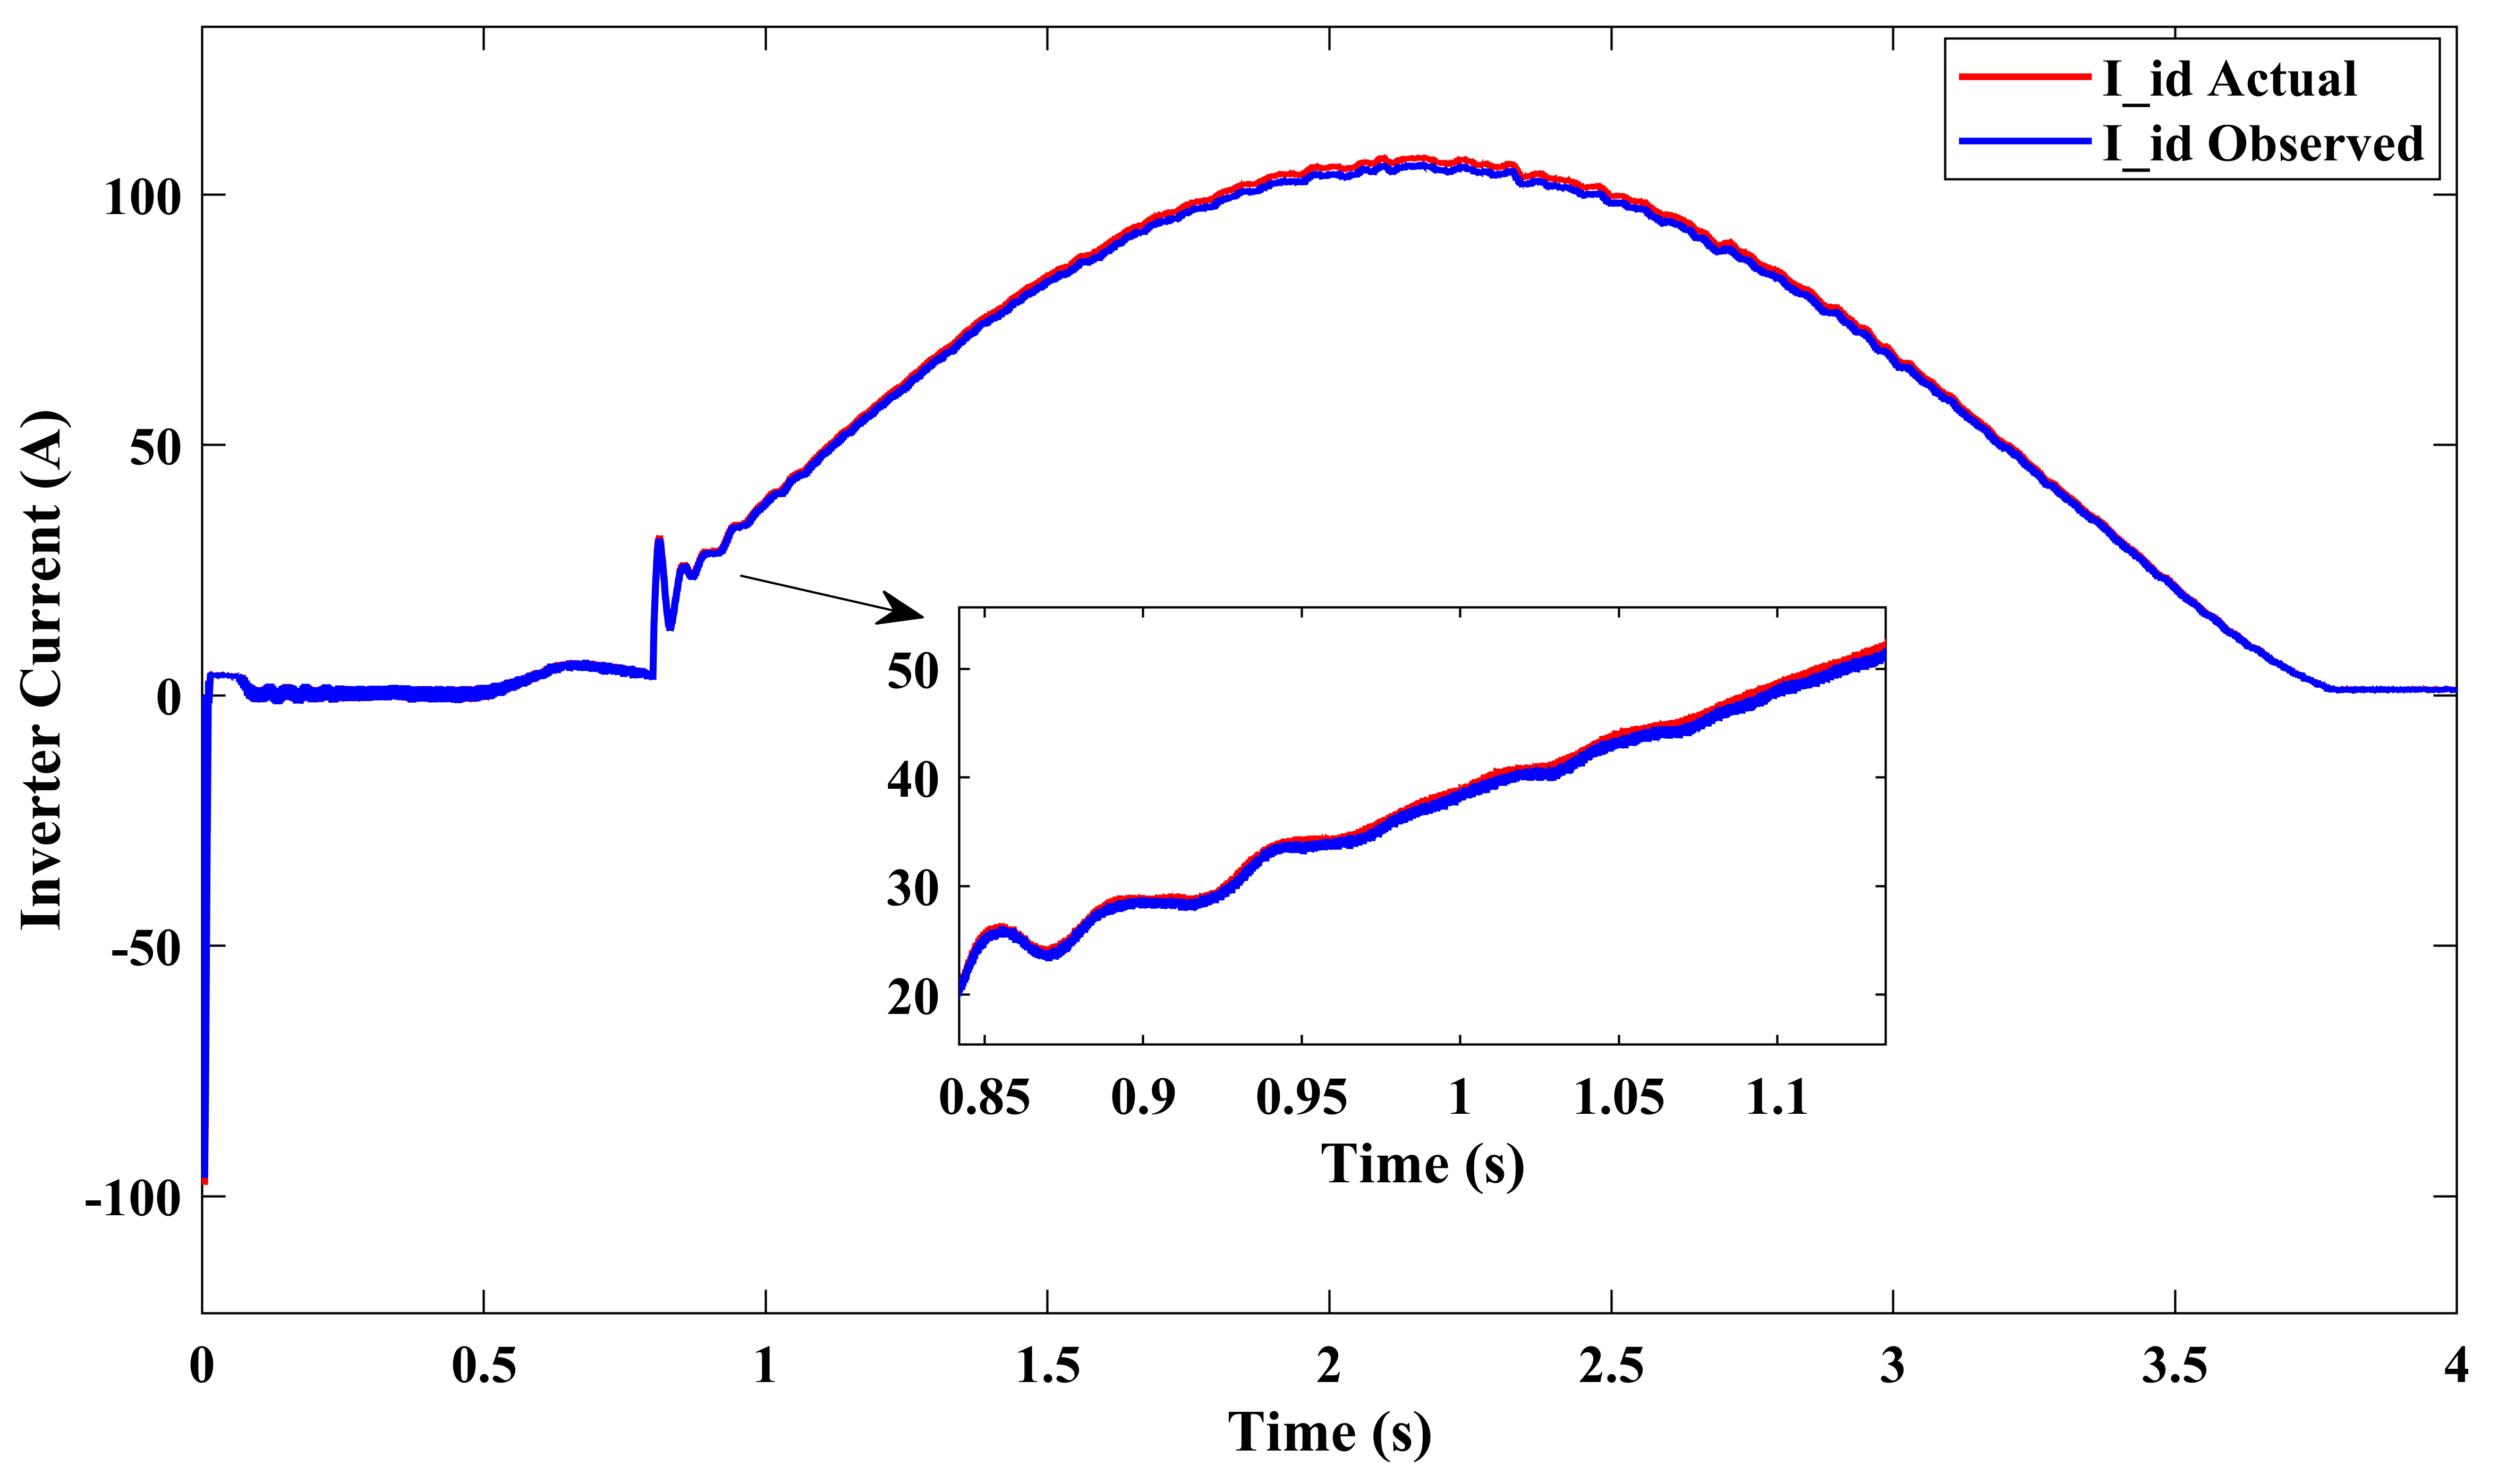
\includegraphics[width=\textwidth,height=4cm,keepaspectratio]{Pictures/Iid Observated.png}
\caption{$I_d$.}
\end{subfigure}\hfill
\begin{subfigure}{0.45\textwidth}
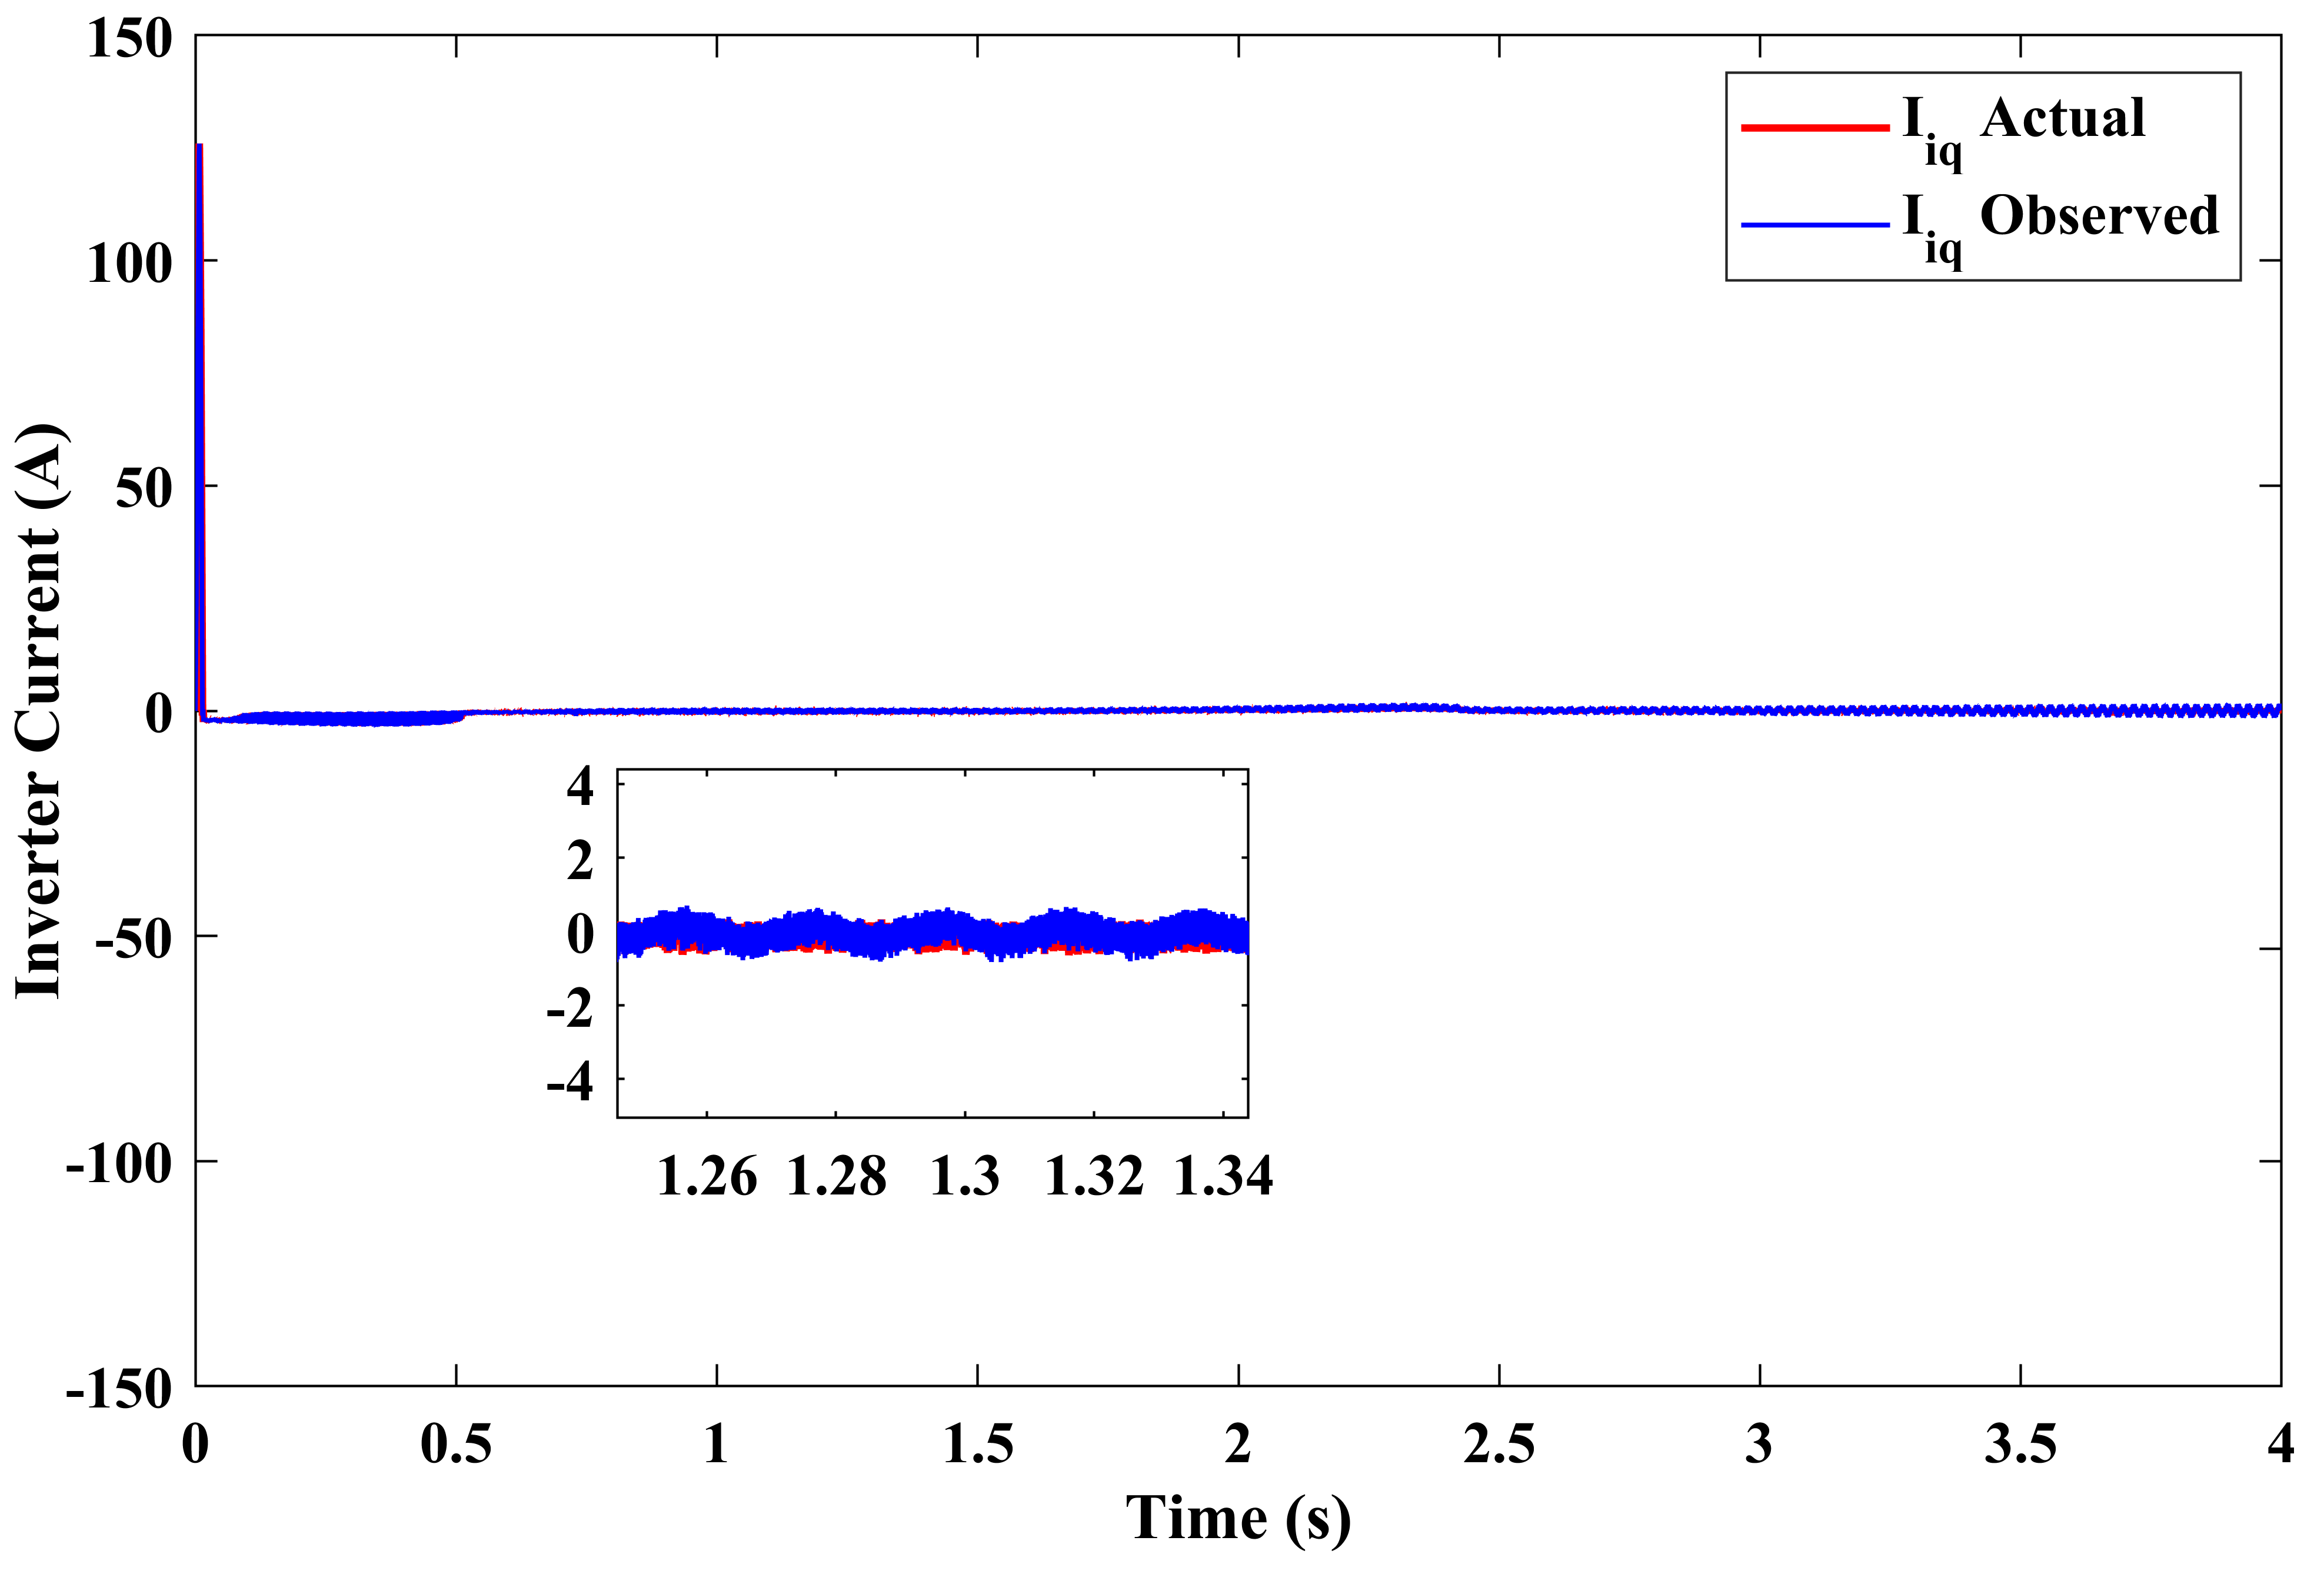
\includegraphics[width=\textwidth,height=4cm,keepaspectratio]{Pictures/Iiq Observed.png}
\caption{$I_q$.}
\end{subfigure}
\caption{Comparison of actual and estimated states.}
\label{fig:observer-results}
\end{figure}

The estimated trajectories follow the corresponding actual states under the tested operating conditions.

\subsection{CTA Performance}

\begin{figure}[htbp]
\centering
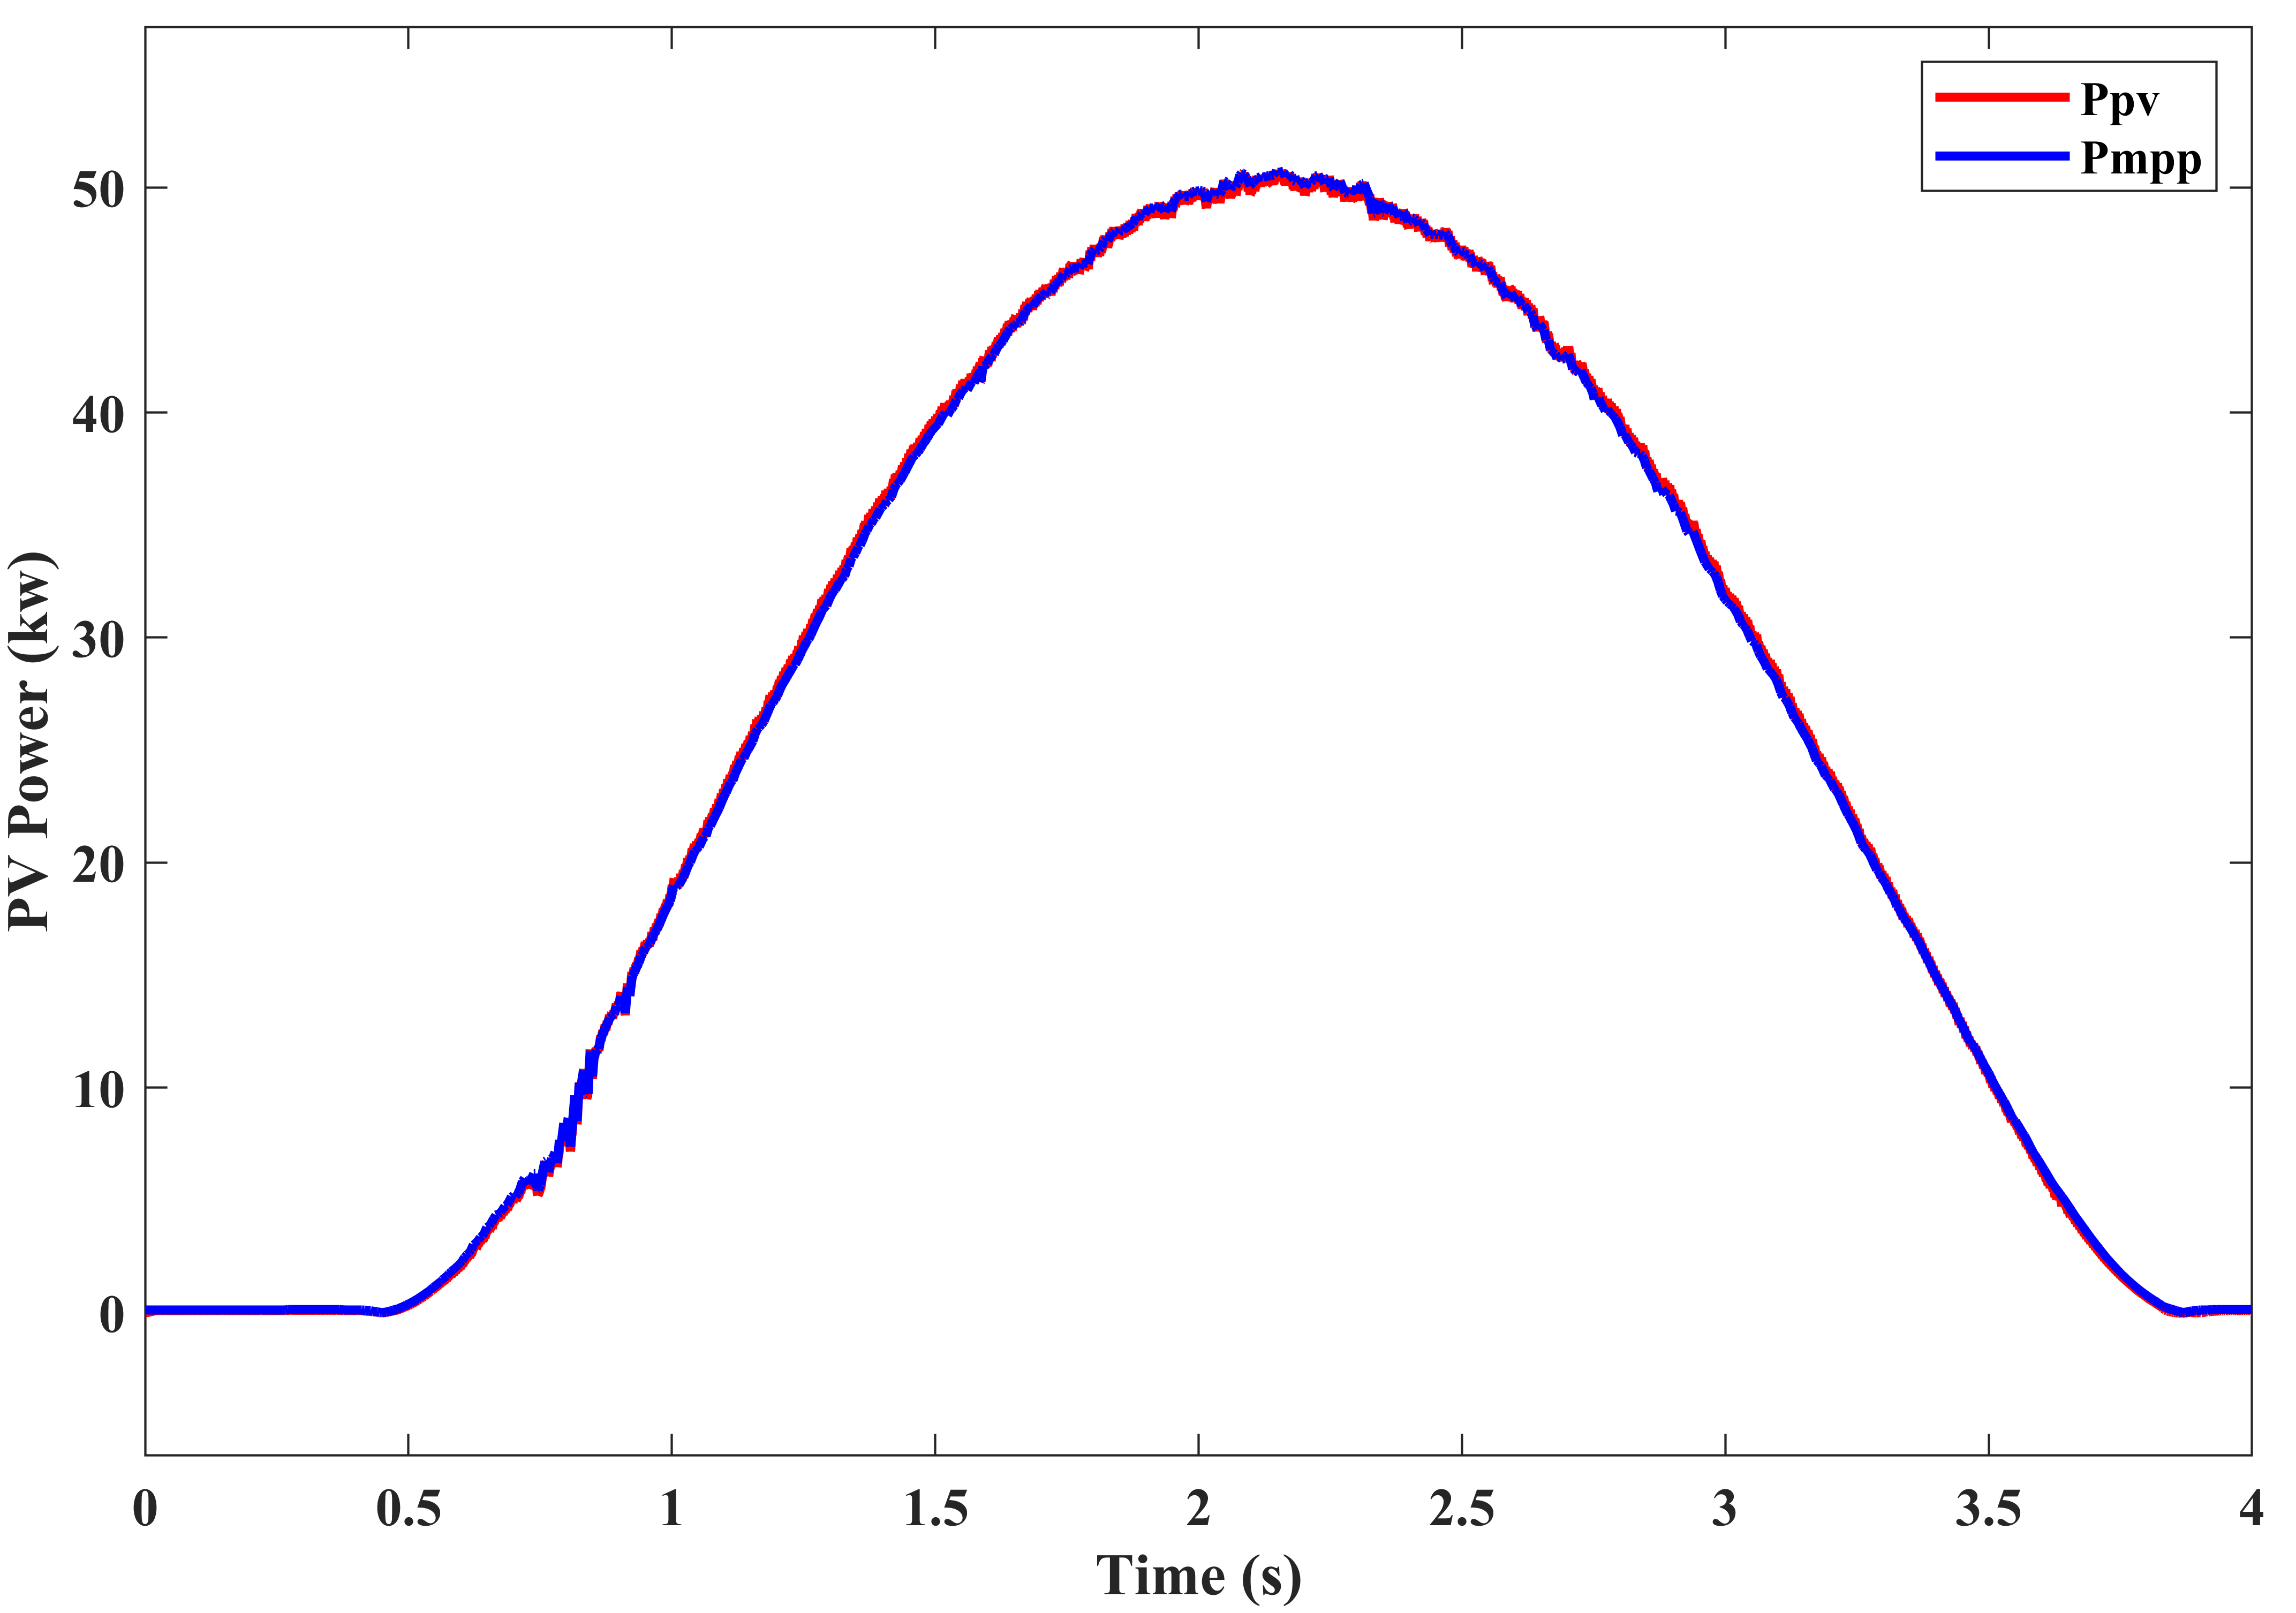
\includegraphics[width=\linewidth]{Pictures/CTA_MPPT.png}
\caption{PV-power tracking obtained using the CTA controller.}
\label{fig:cta-mppt-results}
\end{figure}

\begin{figure}[htbp]
\centering
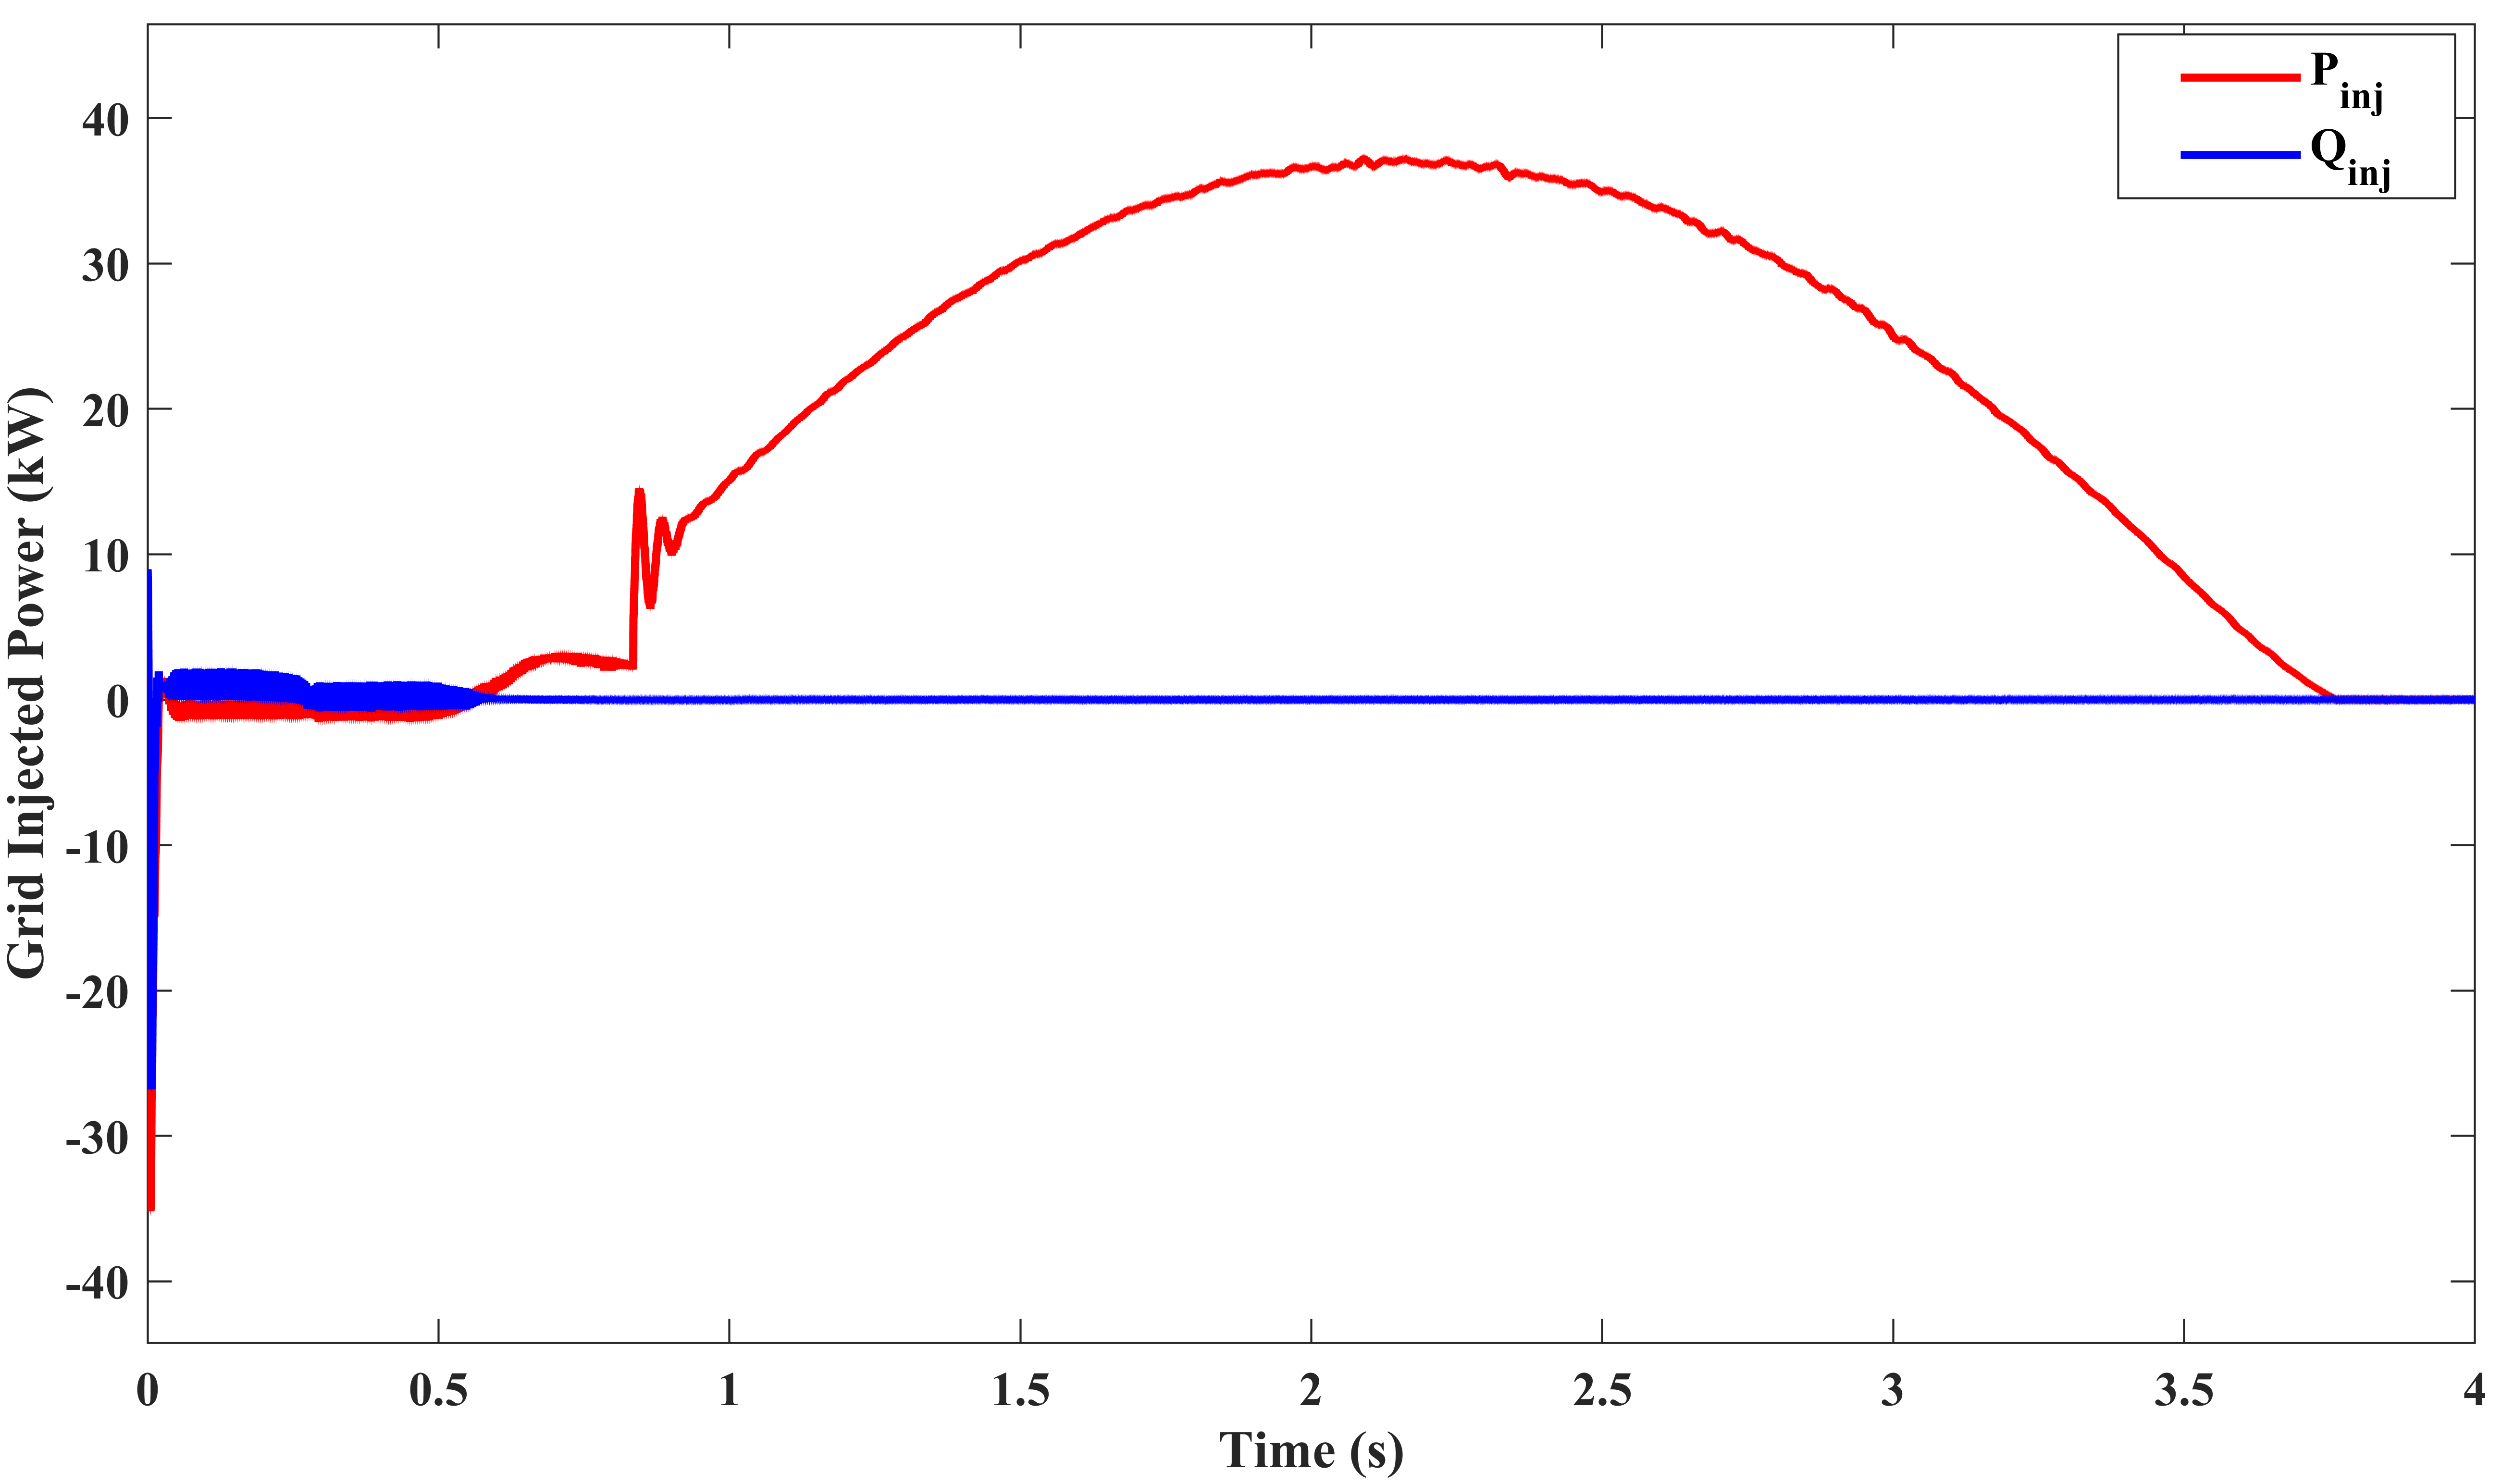
\includegraphics[width=\linewidth]{Pictures/CTA Power injected.png}
\caption{Active power injected into the grid using the CTA controller.}
\label{fig:cta-grid-power}
\end{figure}

\begin{figure}[htbp]
\centering
\begin{subfigure}{0.45\textwidth}
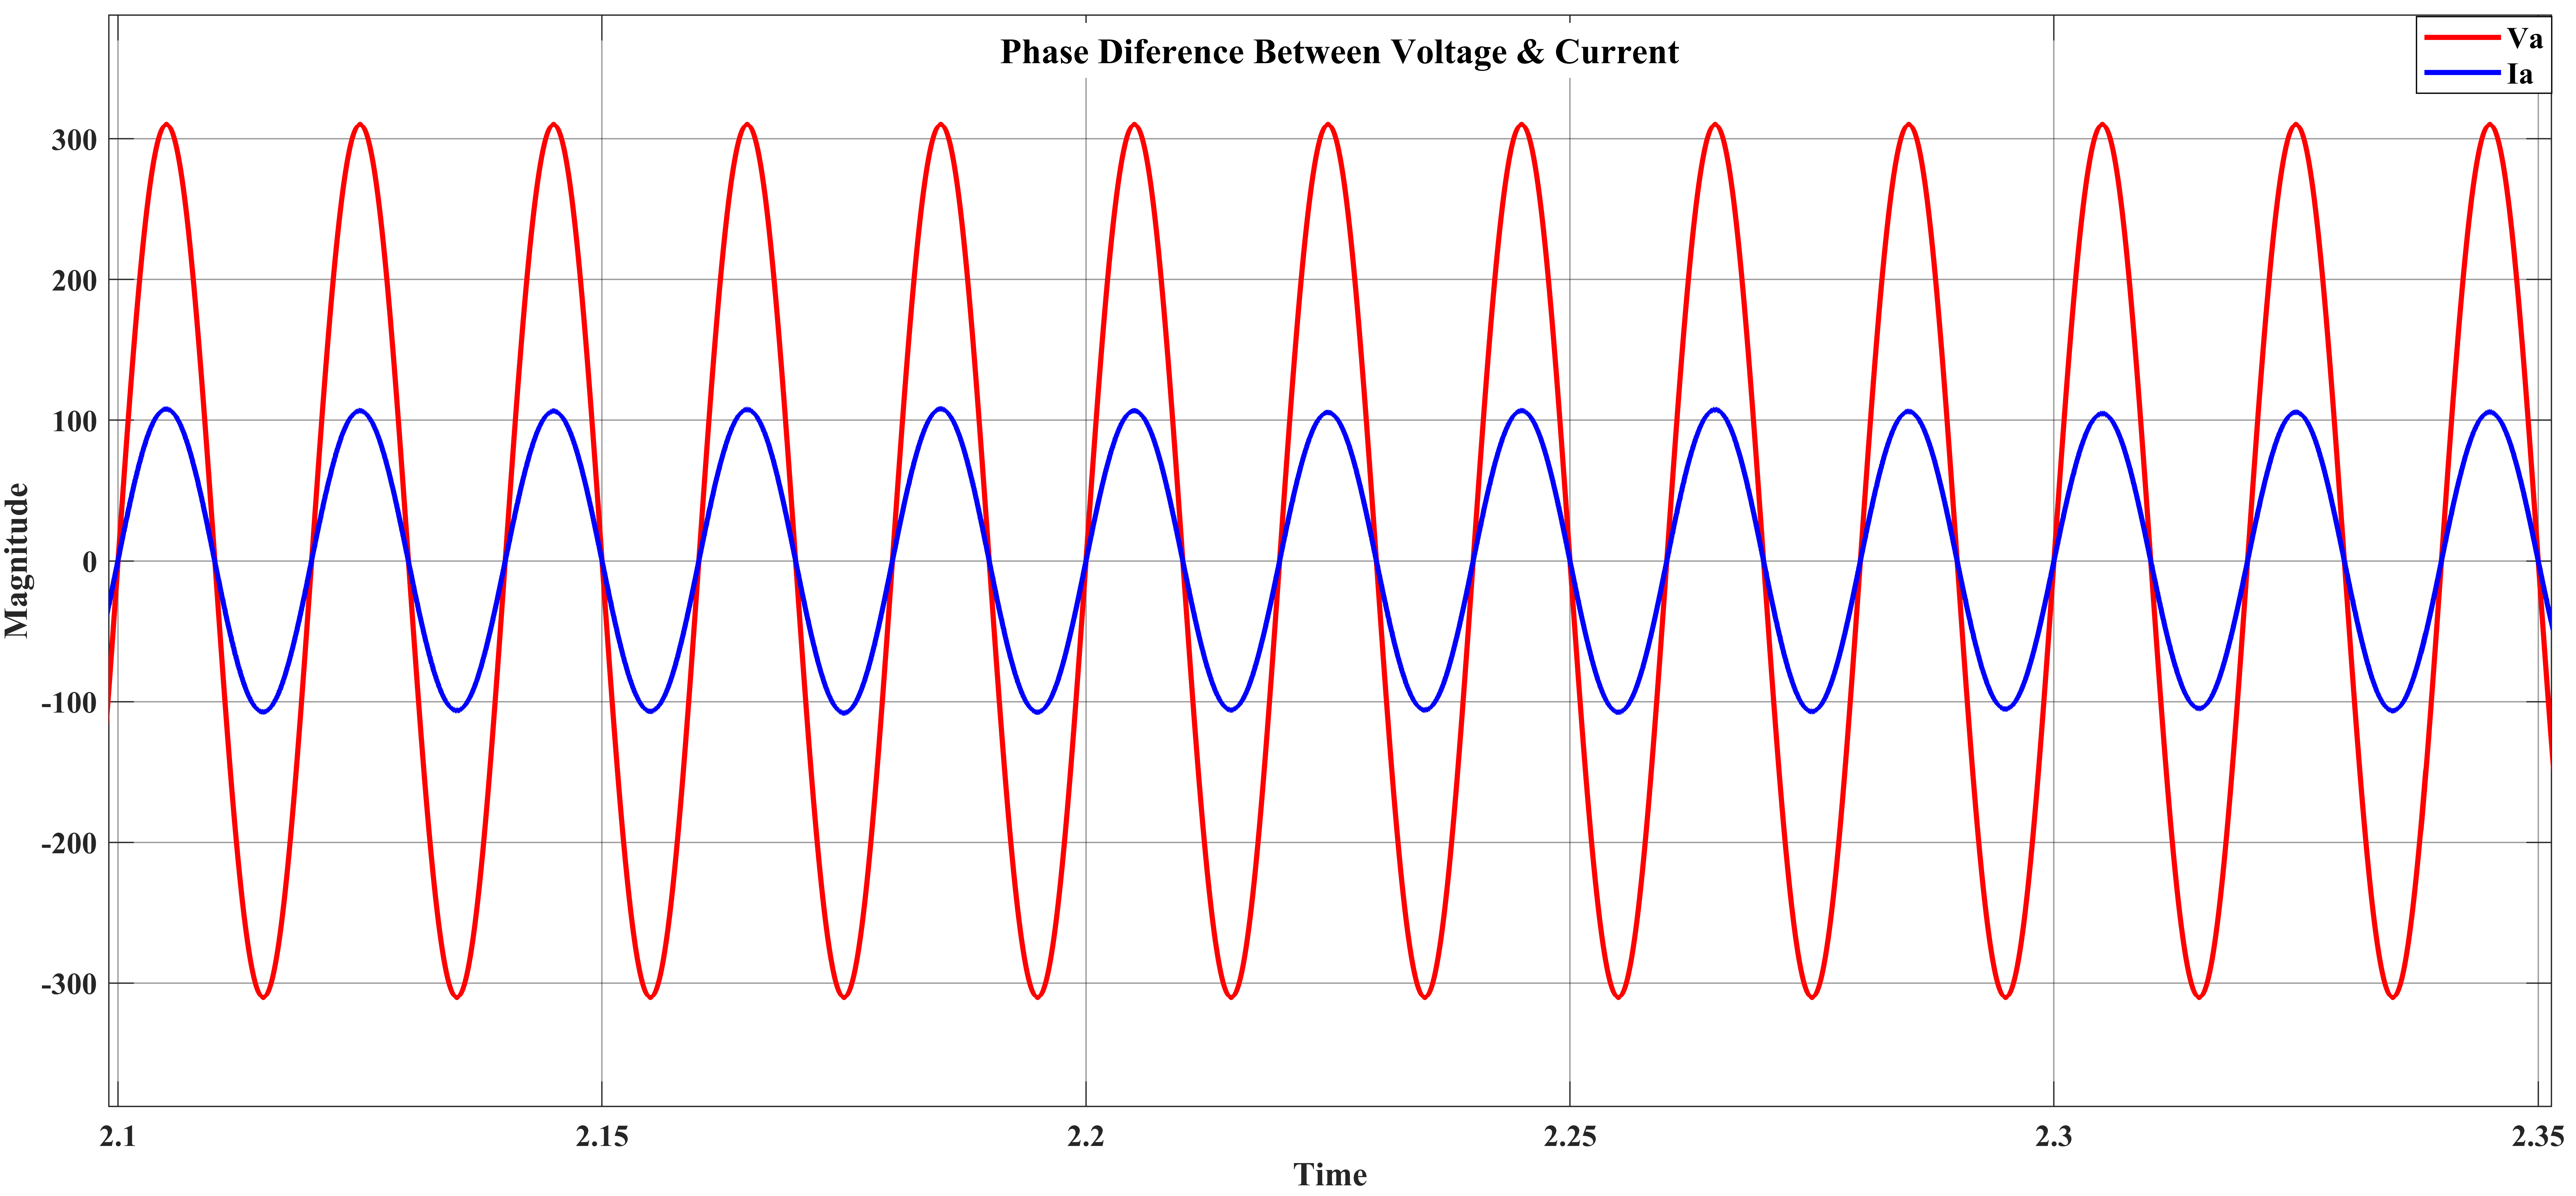
\includegraphics[width=\textwidth,height=4cm,keepaspectratio]{Pictures/CTA_SMC Phase Diference between V & I.png}
\caption{Grid voltage and current.}
\end{subfigure}\hfill
\begin{subfigure}{0.45\textwidth}
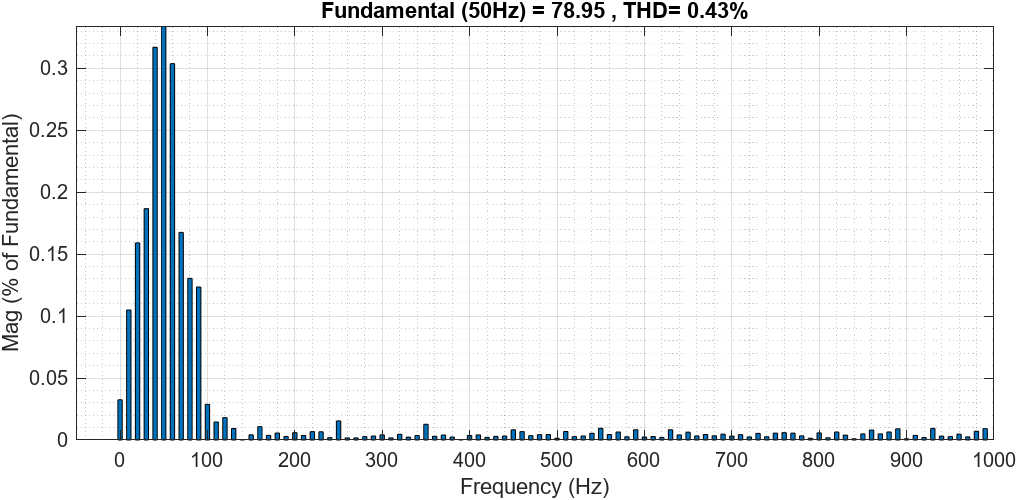
\includegraphics[width=\textwidth,height=4cm,keepaspectratio]{Pictures/CTA_SMC THD 2.png}
\caption{Current harmonic spectrum.}
\end{subfigure}
\caption{CTA grid-side power-quality responses.}
\label{fig:cta-power-quality}
\end{figure}

The reported CTA grid-current THD is $0.43\%$.

\subsection{DIC Performance}

\begin{figure}[htbp]
\centering
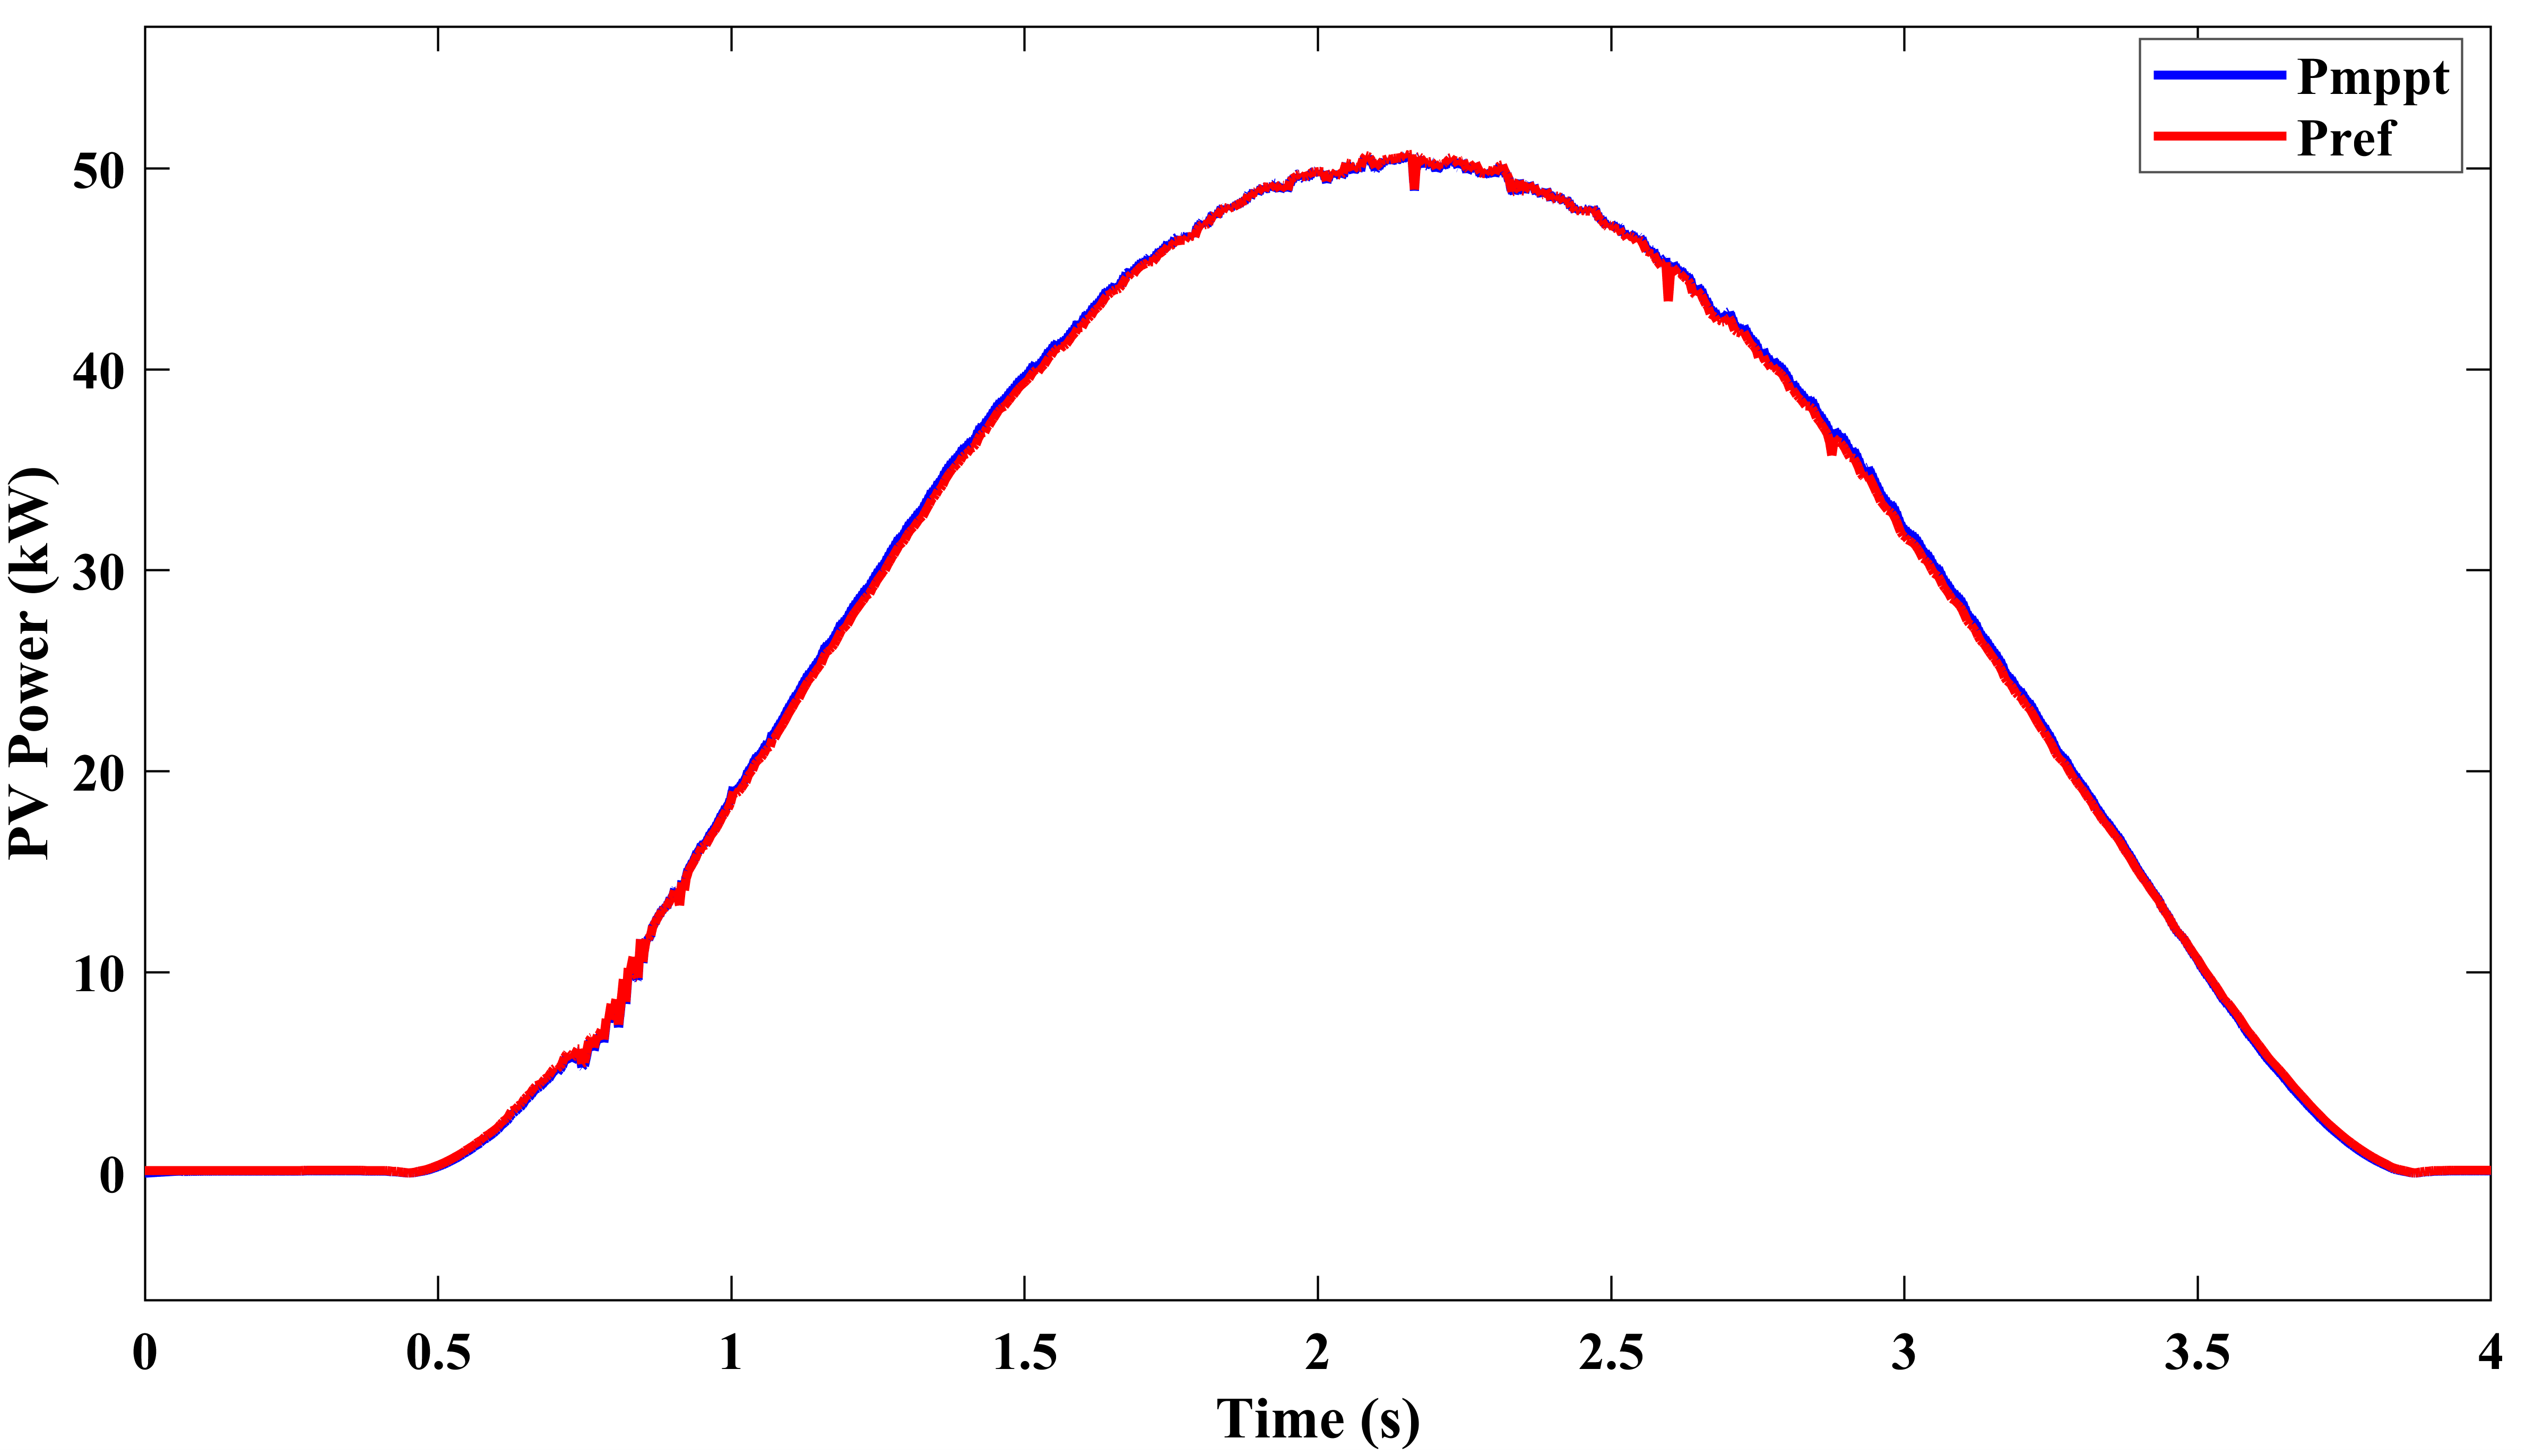
\includegraphics[width=\linewidth]{Pictures/DIC_MPPT.png}
\caption{PV-power tracking obtained using the DIC controller.}
\label{fig:dic-mppt-results}
\end{figure}

\begin{figure}[htbp]
\centering
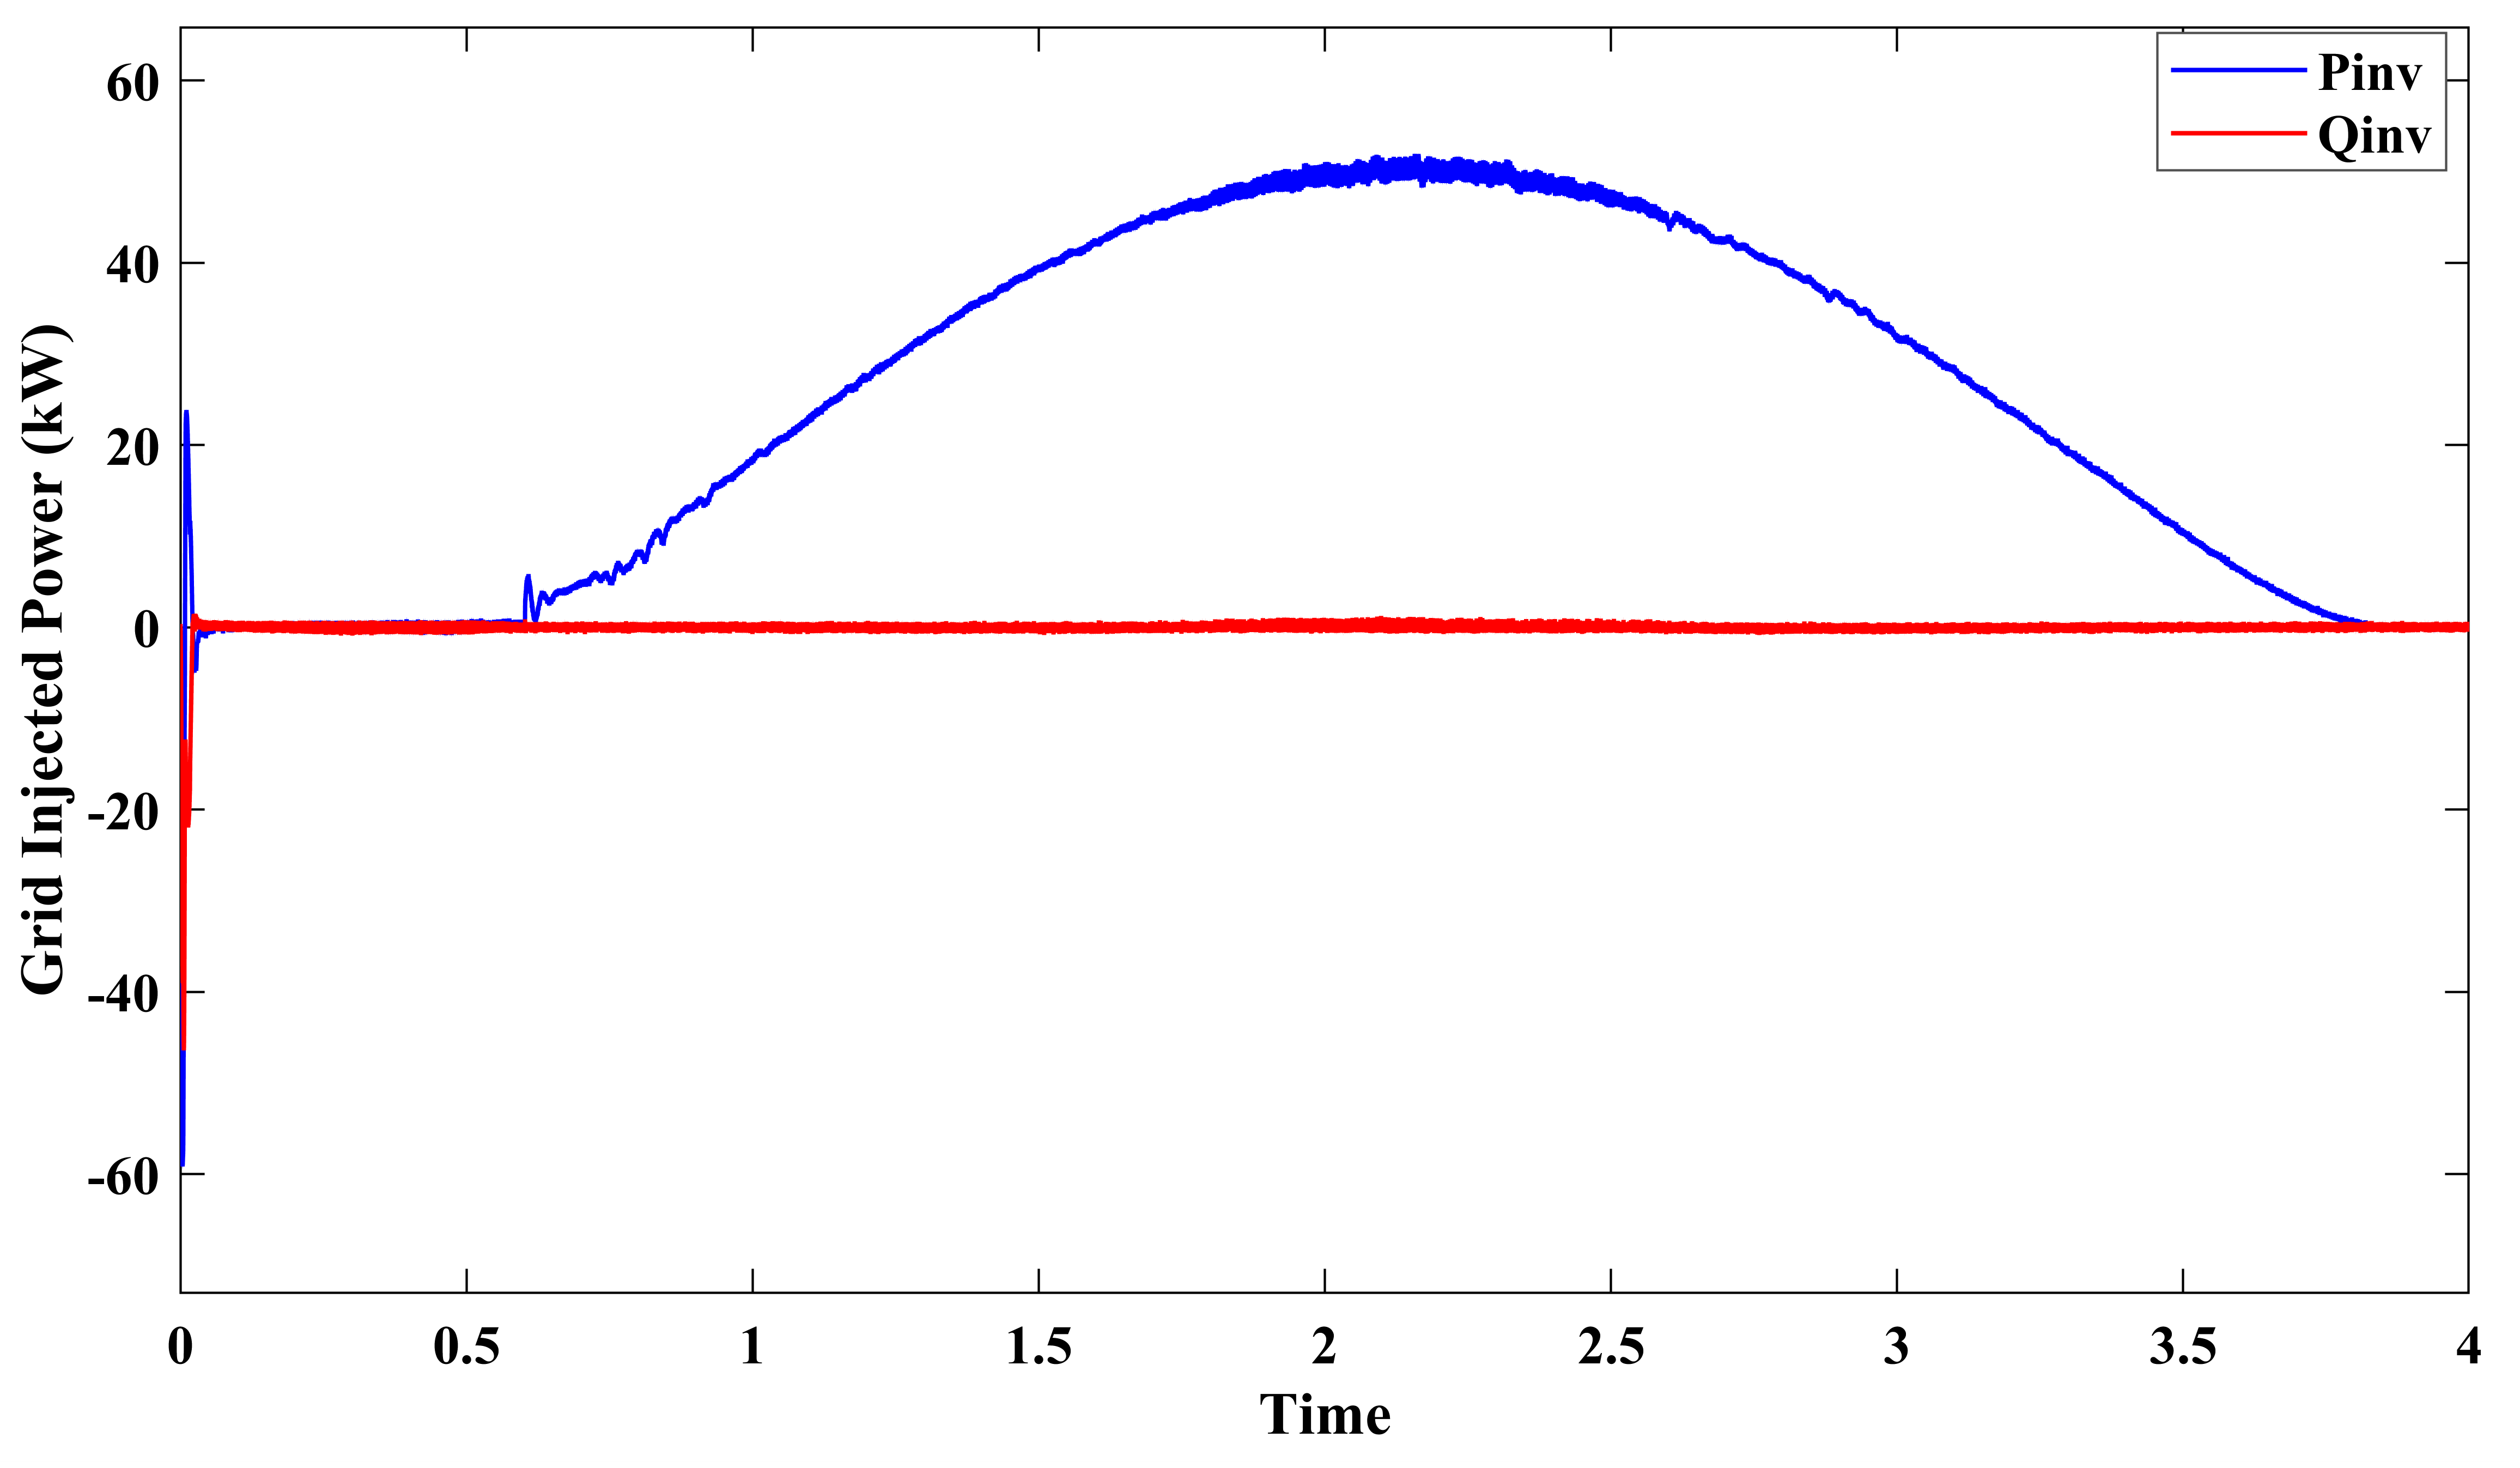
\includegraphics[width=\linewidth]{Pictures/DIC Power injected.png}
\caption{Active power injected into the grid using the DIC controller.}
\label{fig:dic-grid-power}
\end{figure}

\begin{figure}[htbp]
\centering
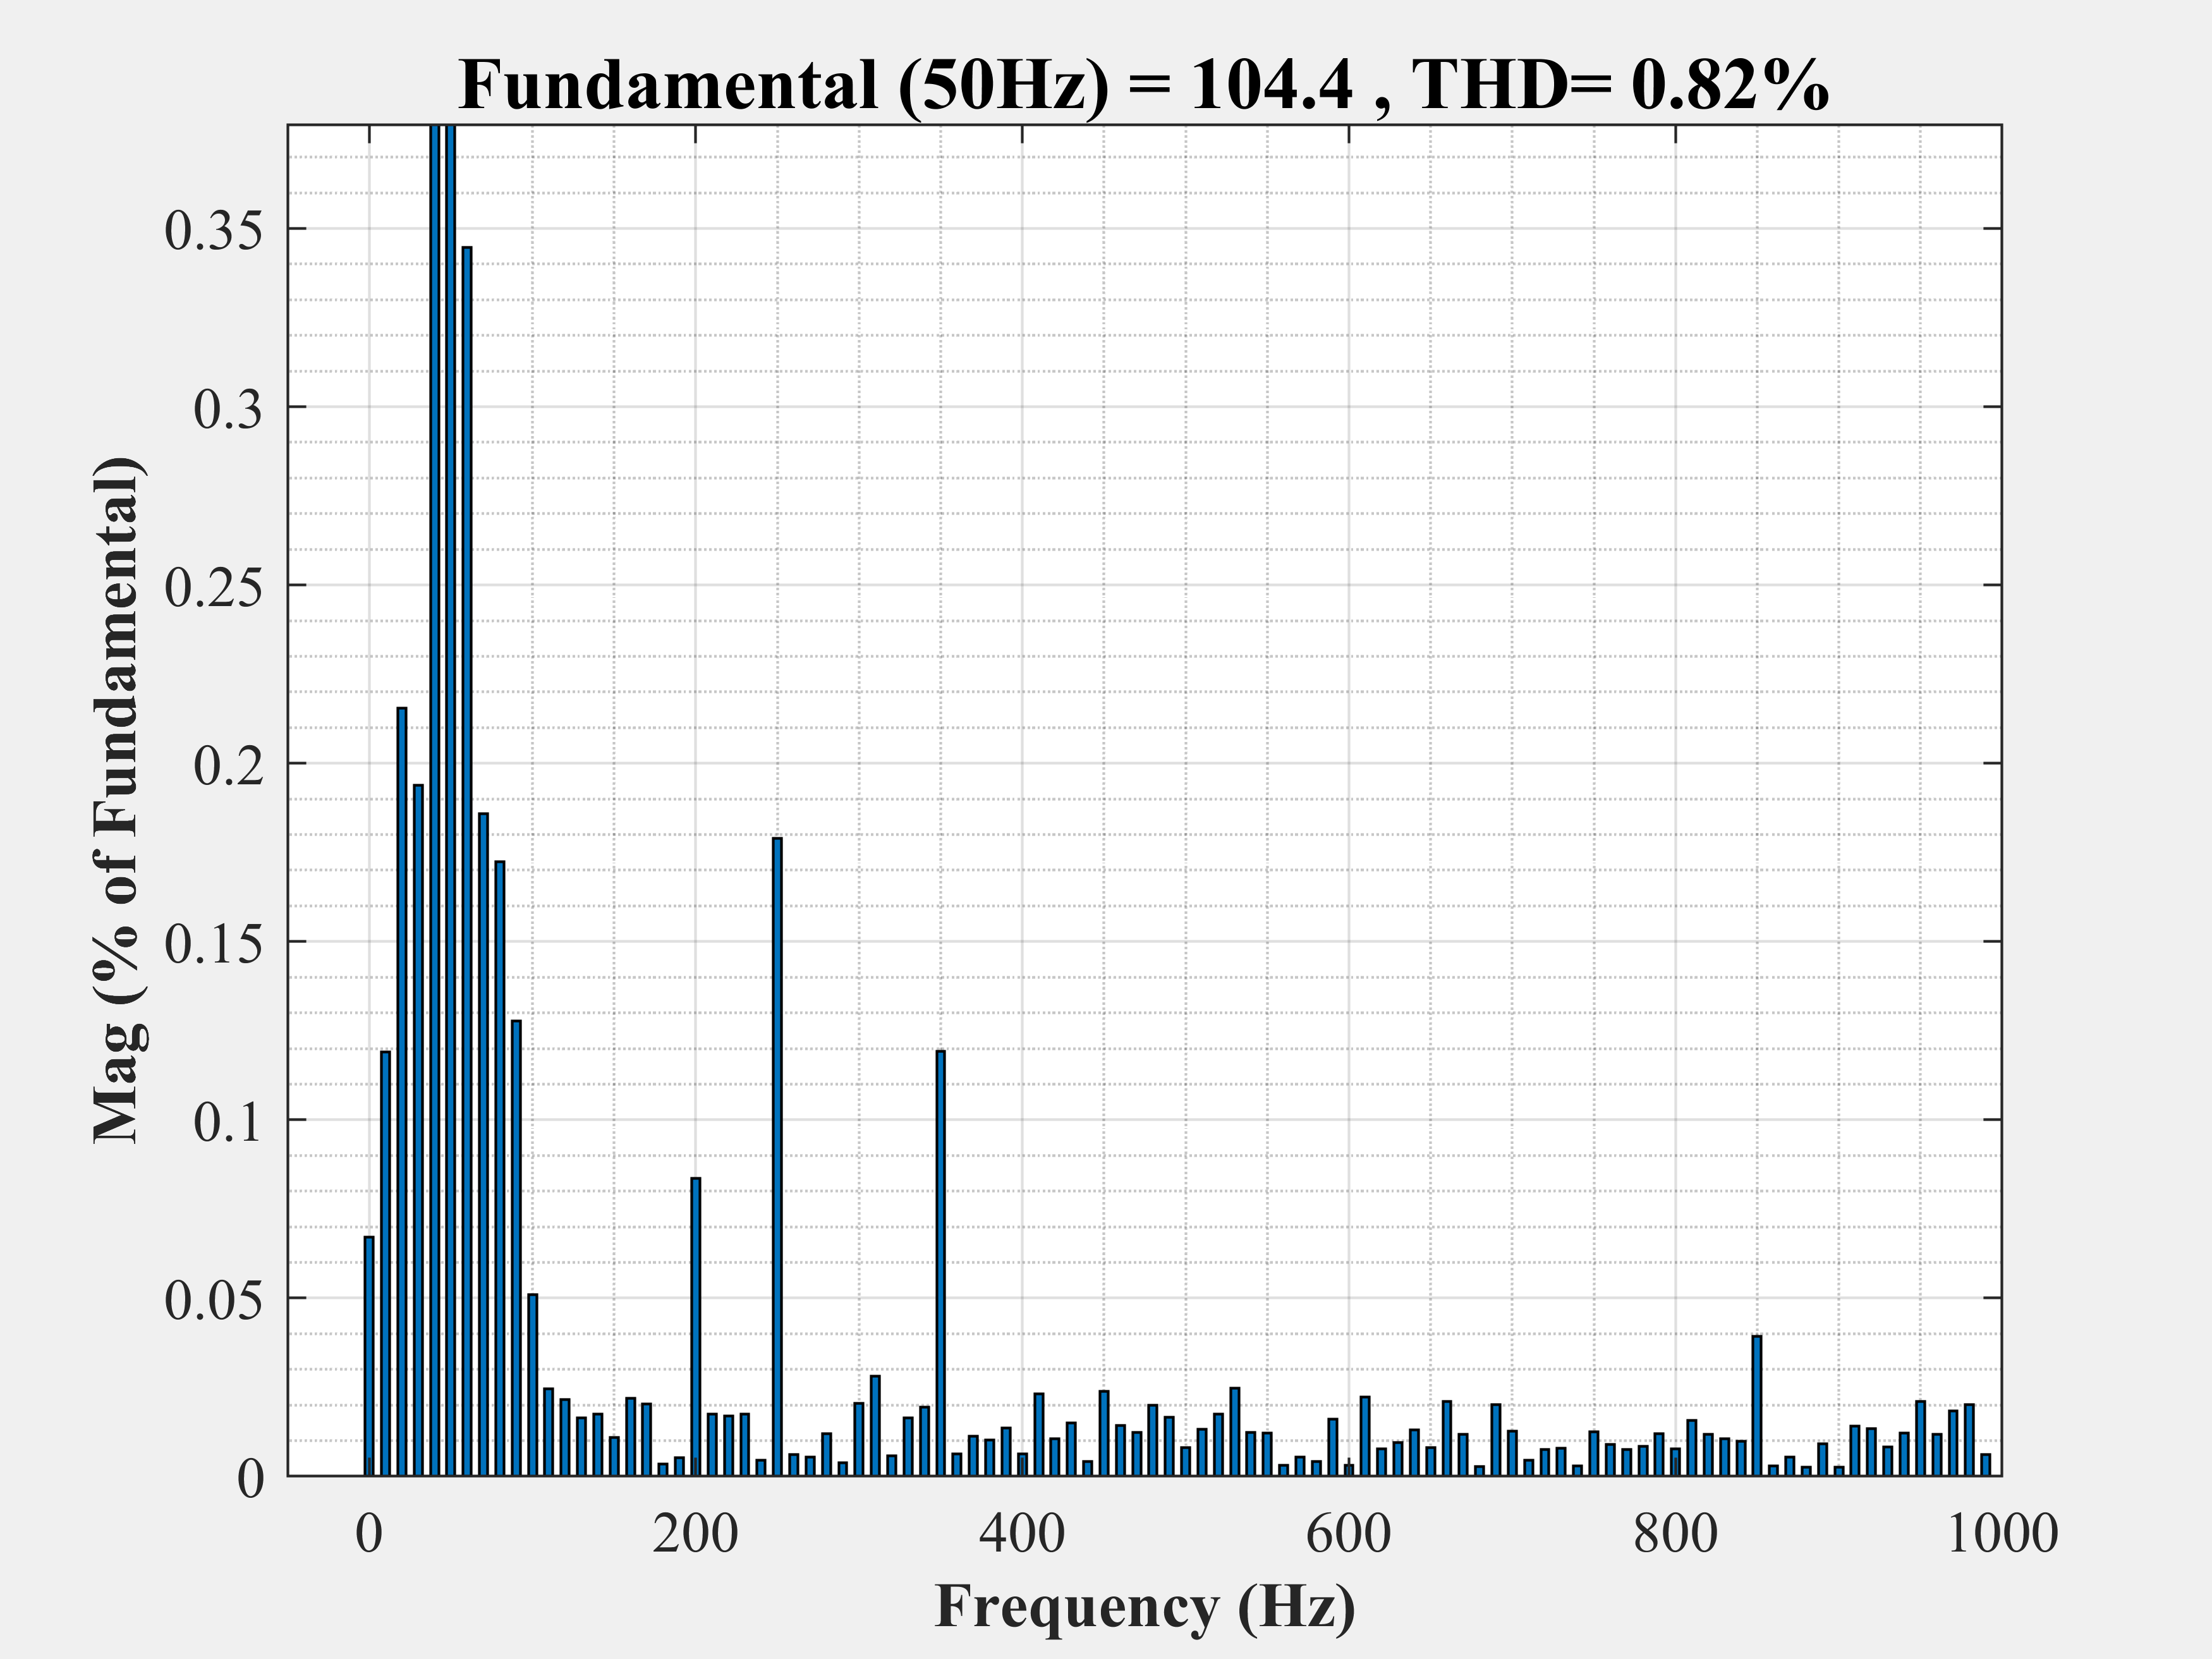
\includegraphics[width=\linewidth]{Pictures/DIC_SMC THD.png}
\caption{Grid-current harmonic spectrum obtained using the DIC controller.}
\label{fig:dic-grid-thd}
\end{figure}

\begin{figure}[htbp]
\centering
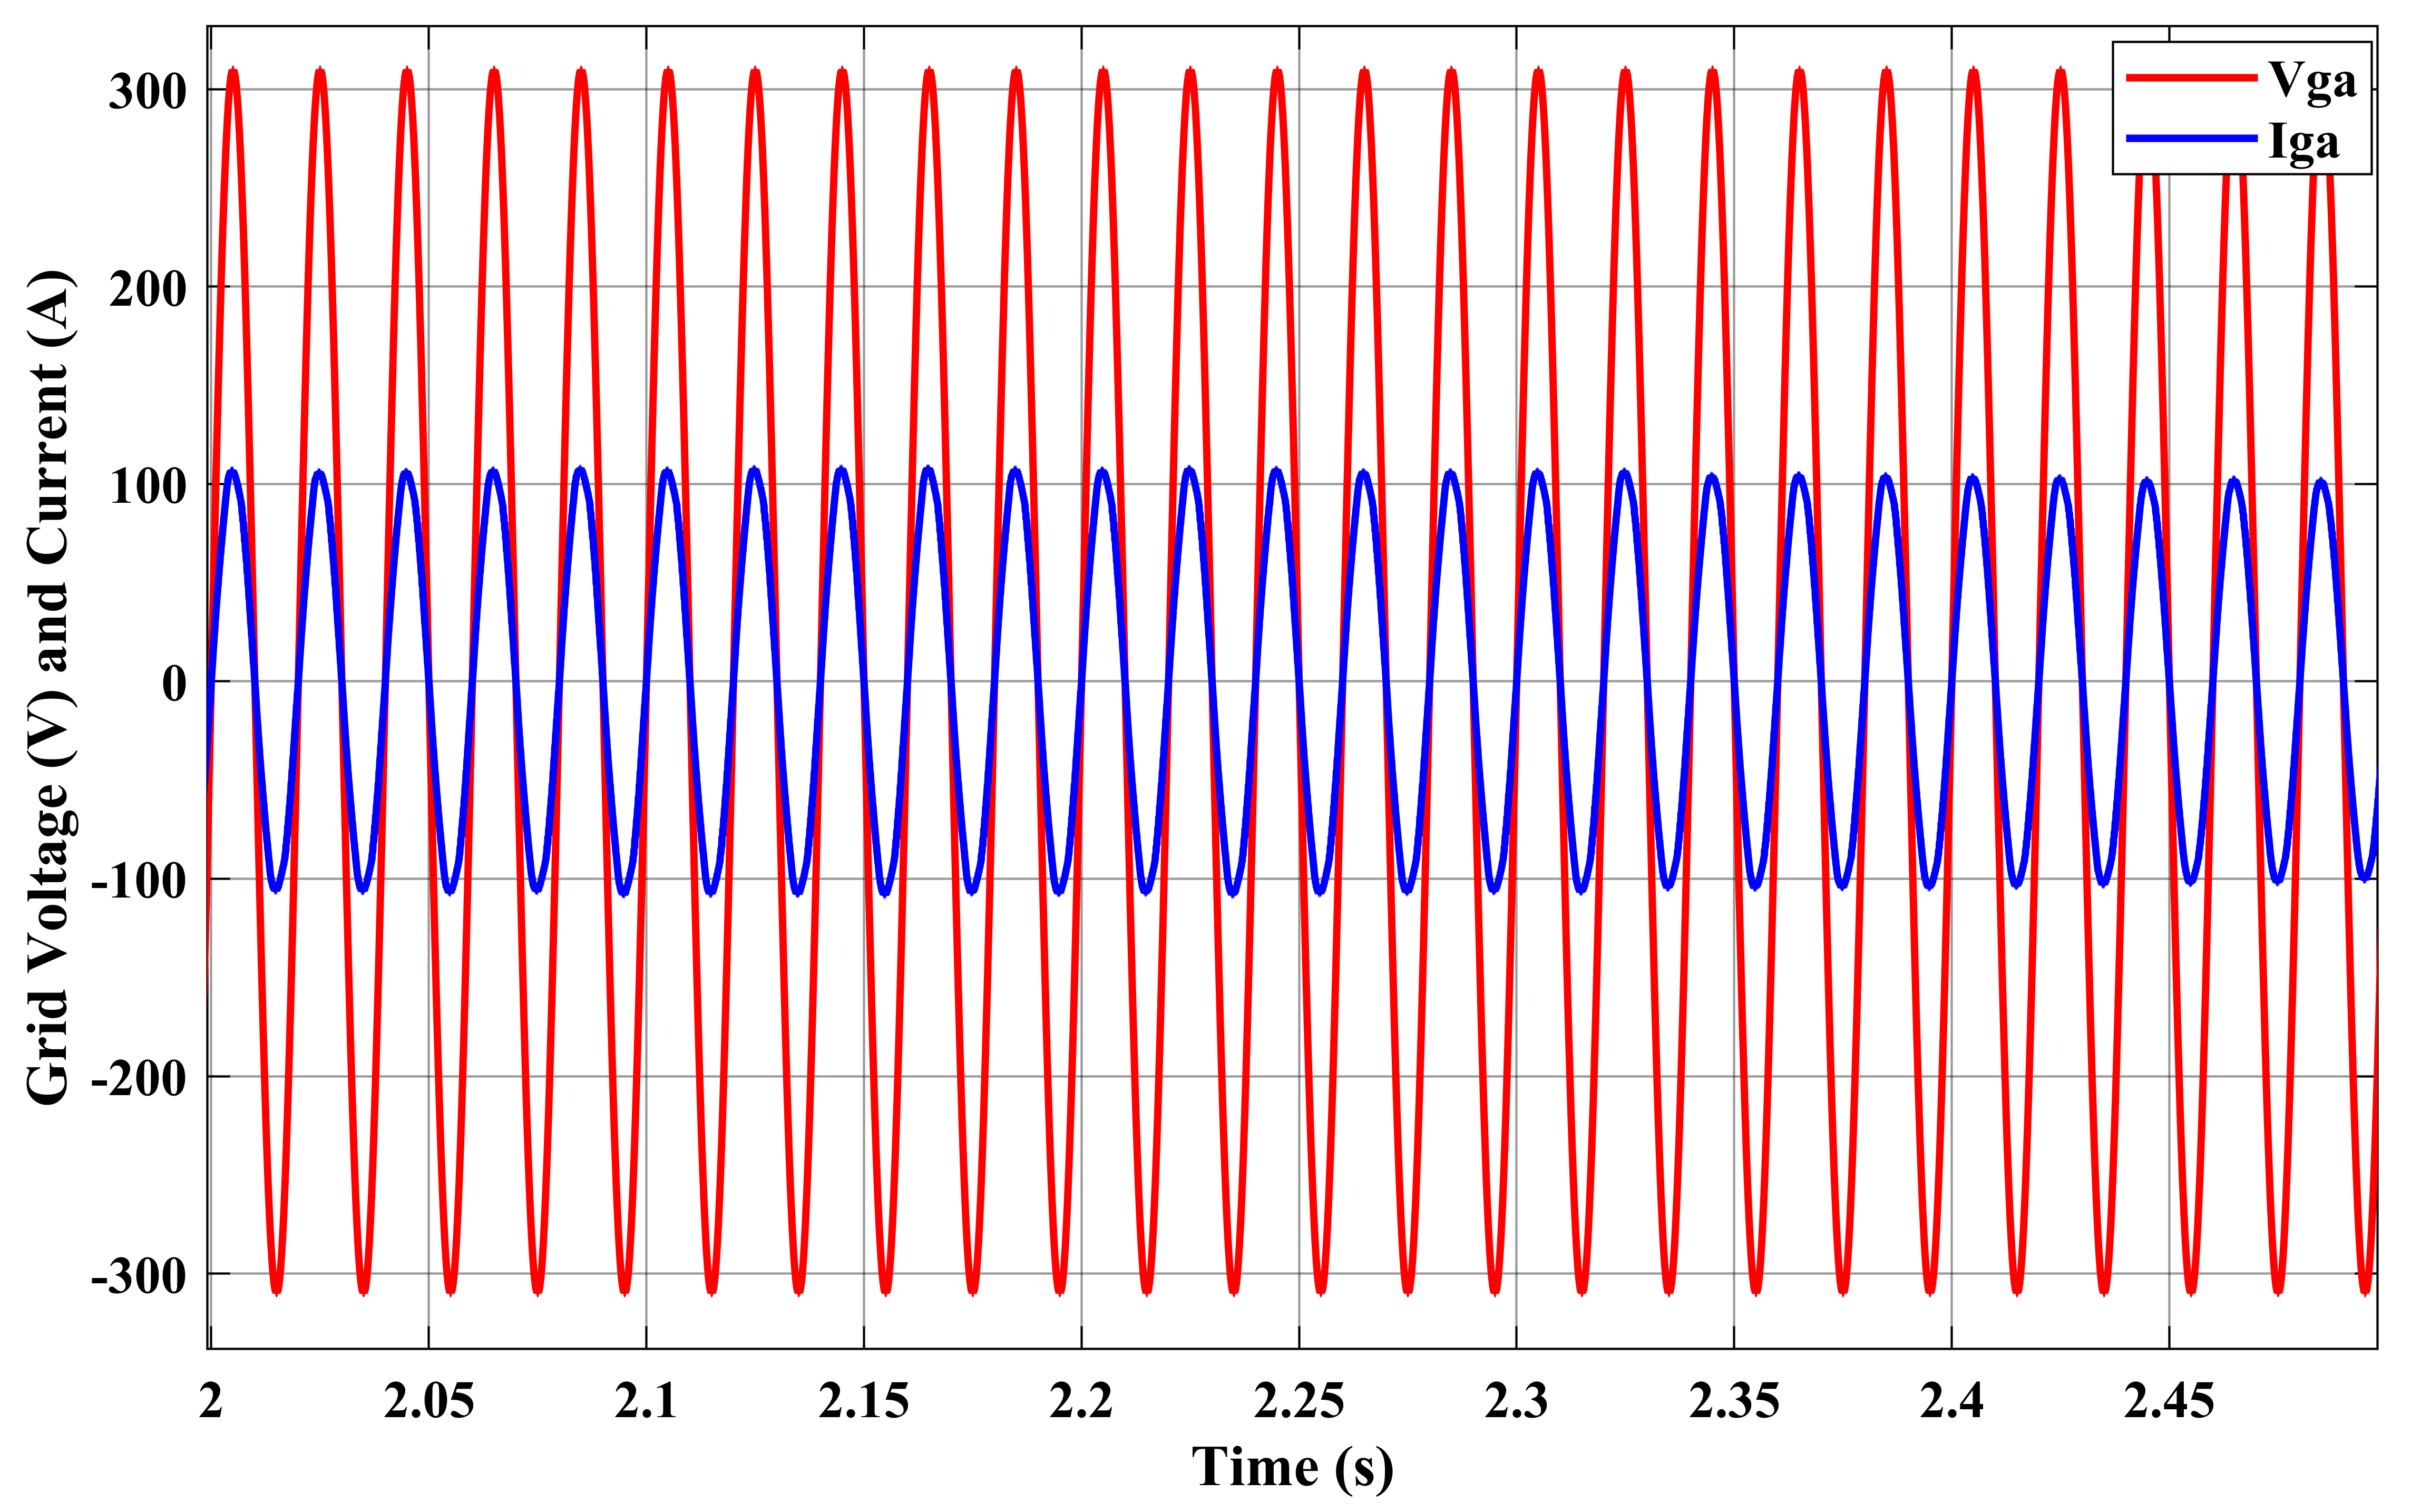
\includegraphics[width=\linewidth]{Pictures/DIC Grid voltage and current.png}
\caption{Grid voltage and current obtained using the DIC controller.}
\label{fig:dic-grid-sync}
\end{figure}

The reported DIC grid-current THD is $0.82\%$.

\section{Comparative Analysis}
\label{sec:comparison}

The dynamic MPPT efficiency is
\begin{equation}
\eta_{\mathrm{MPPT}}=\frac{\int_{t_0}^{t_f}P_{pv}(t)\,dt}{\int_{t_0}^{t_f}P_{\mathrm{ref}}(t)\,dt}\times100\%.
\label{eq:mppt-efficiency}
\end{equation}
For $t_0=0~\mathrm{s}$ and $t_f=4~\mathrm{s}$, the CTA, DIC, and PI controllers achieved $99.4\%$, $98.0\%$, and $95.0\%$, respectively.

\begin{figure}[htbp]
\centering
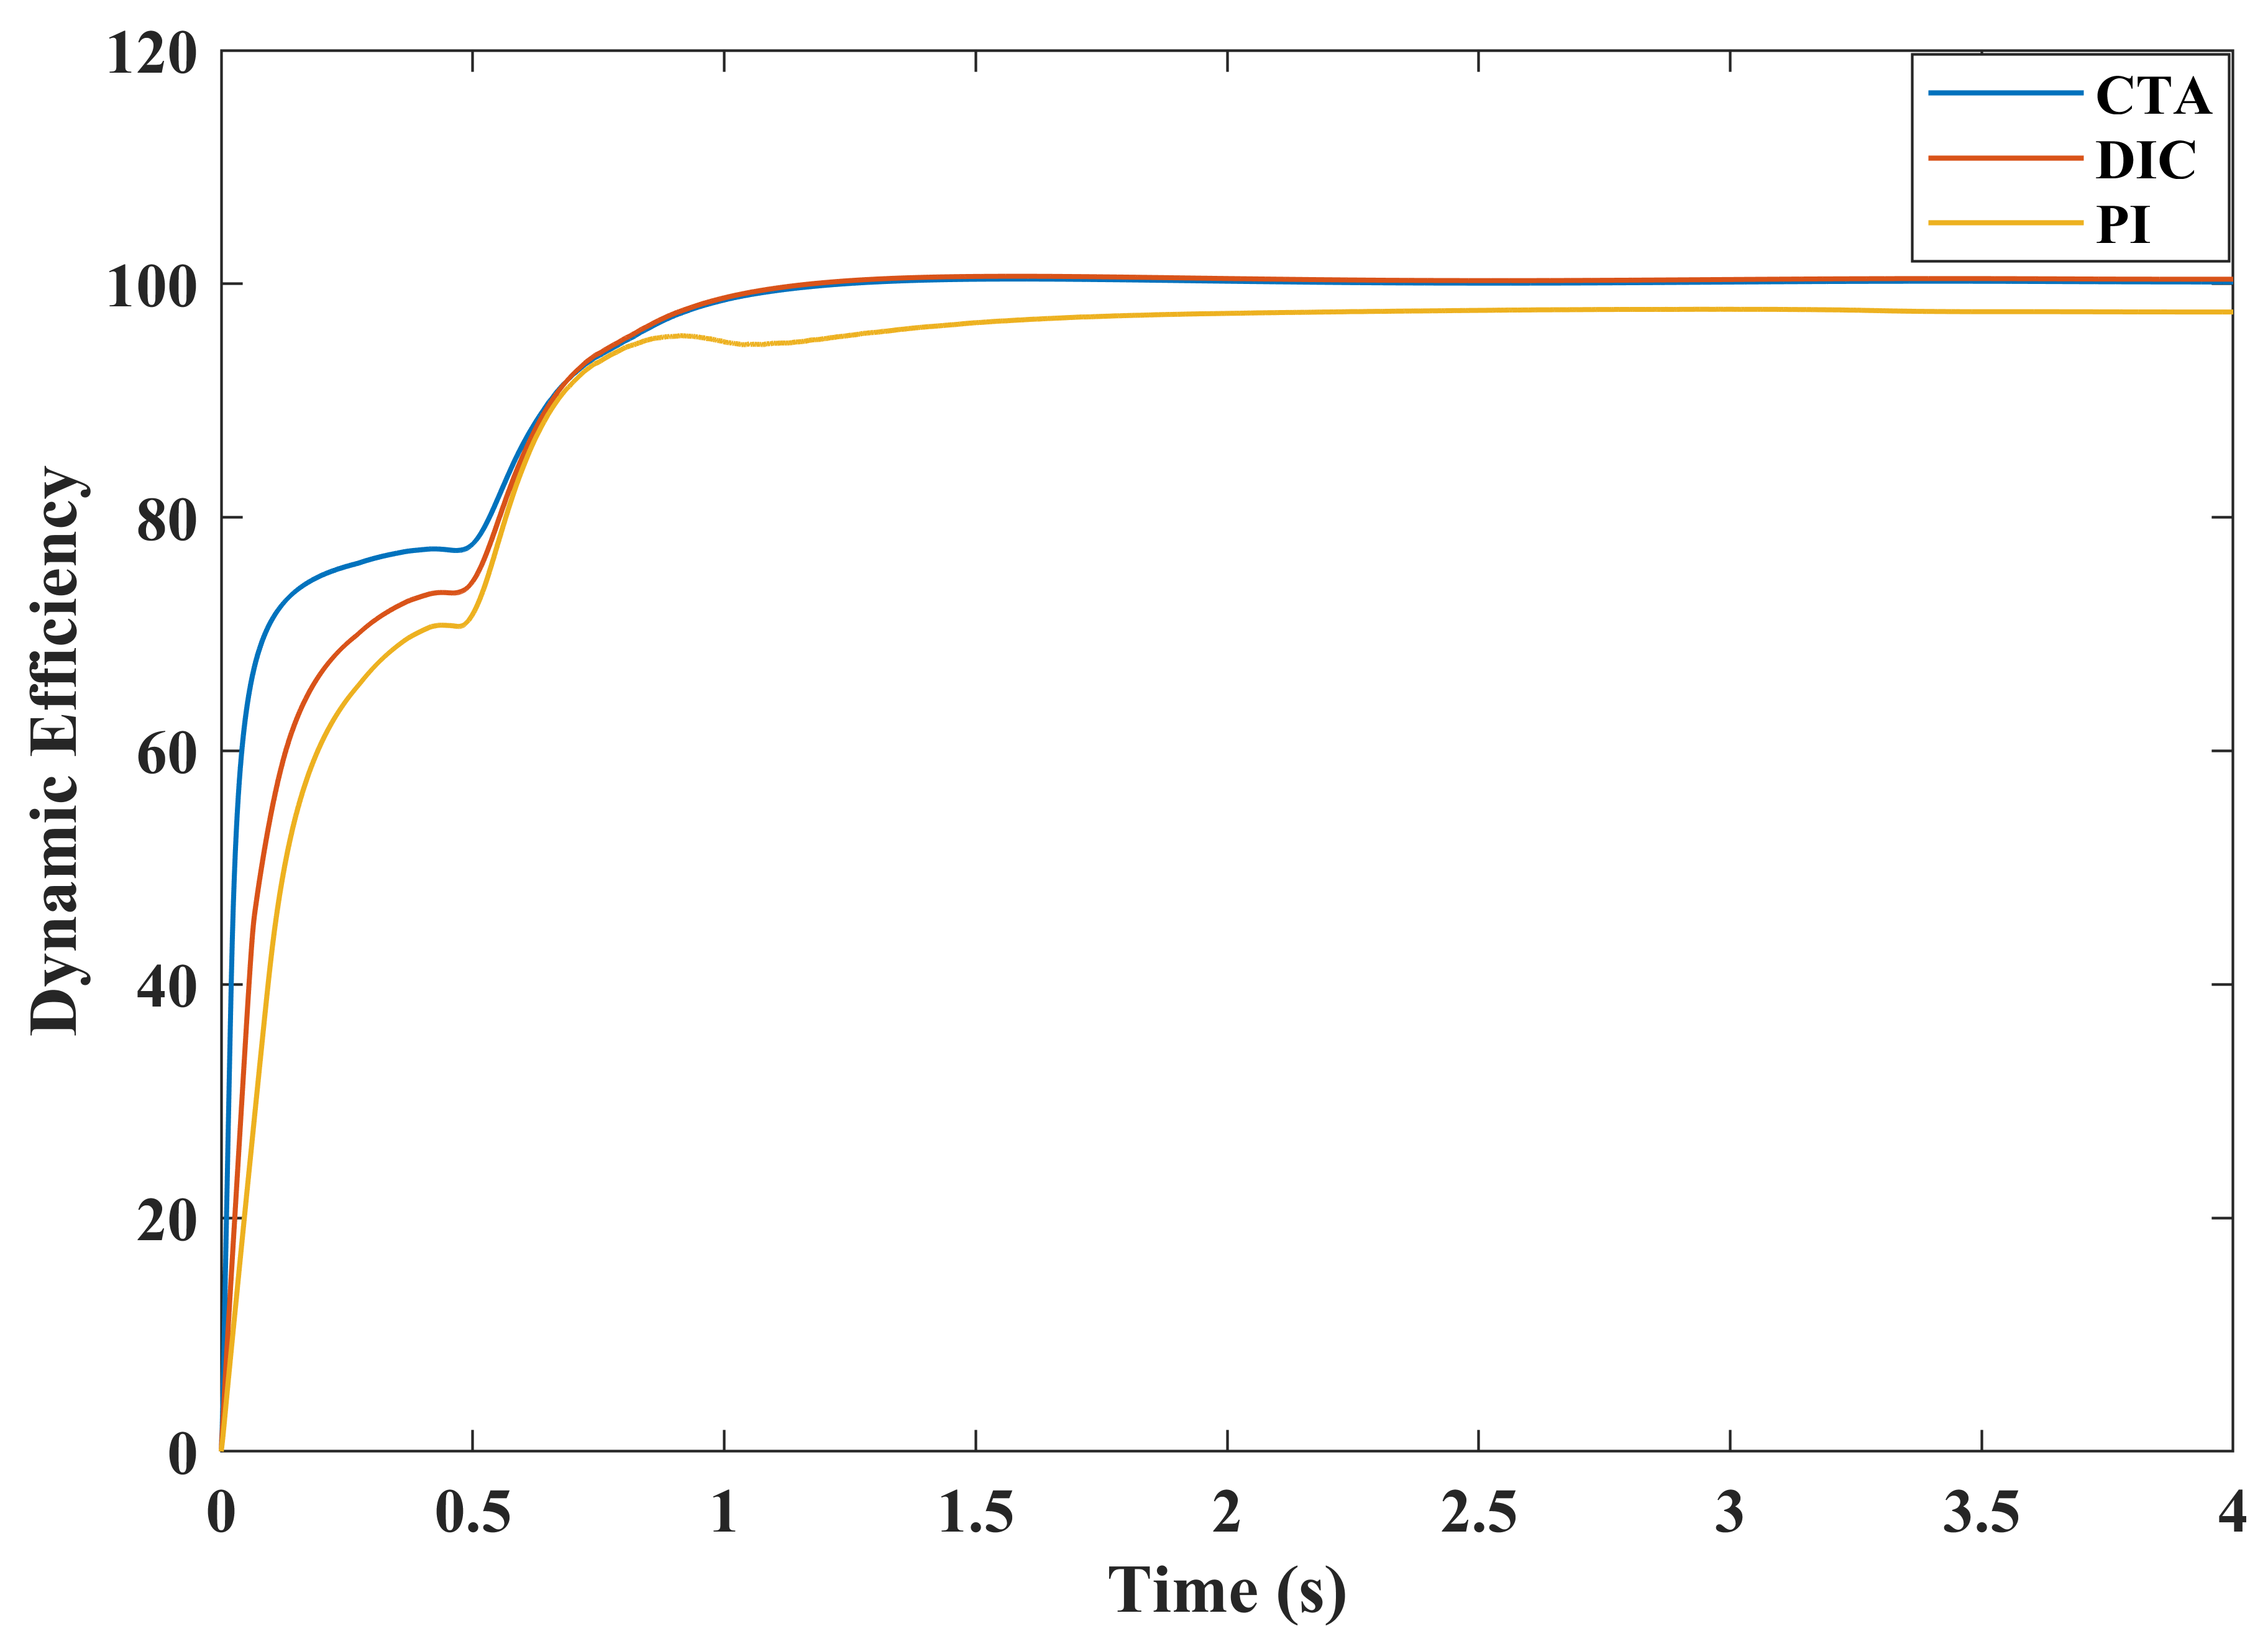
\includegraphics[width=\linewidth]{Pictures/Dynamic efficiency.png}
\caption{Dynamic MPPT efficiencies.}
\label{fig:dynamic-efficiency}
\end{figure}

\begin{figure}[htbp]
\centering
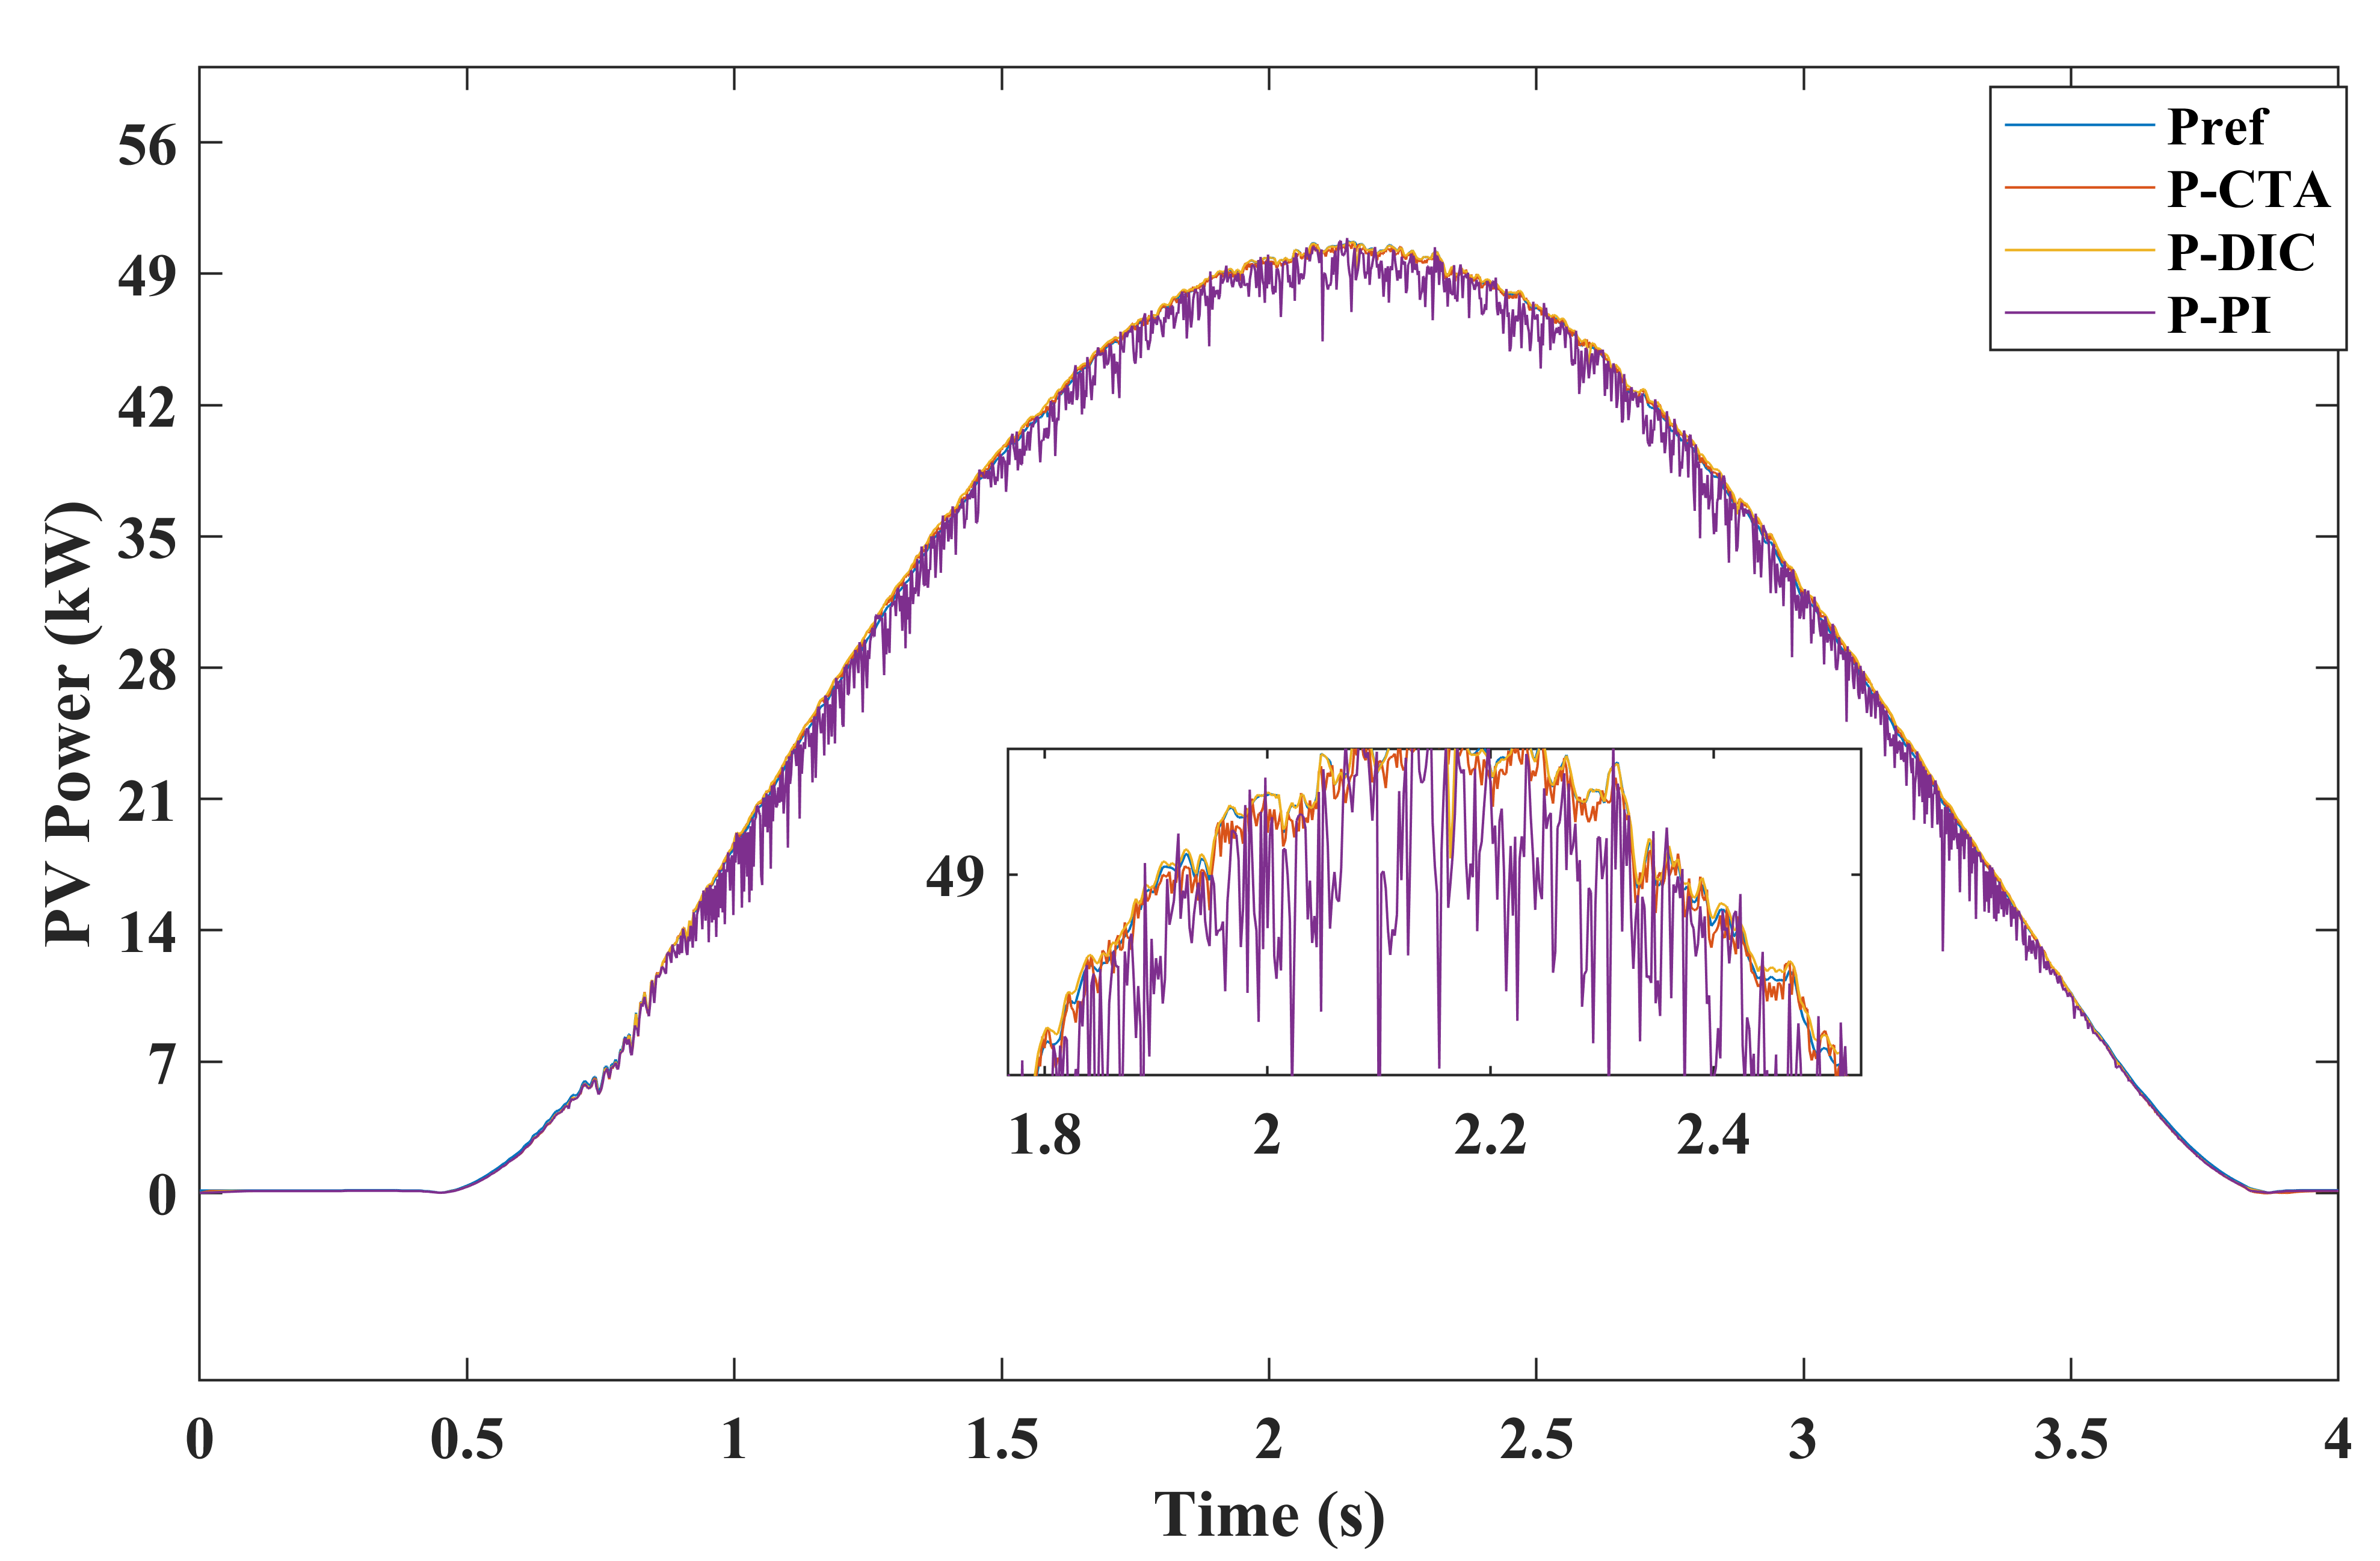
\includegraphics[width=\linewidth]{Pictures/MPPT Comparison.png}
\caption{Comparison of PV-power tracking responses.}
\label{fig:mppt-comparison}
\end{figure}

\begin{figure}[htbp]
\centering
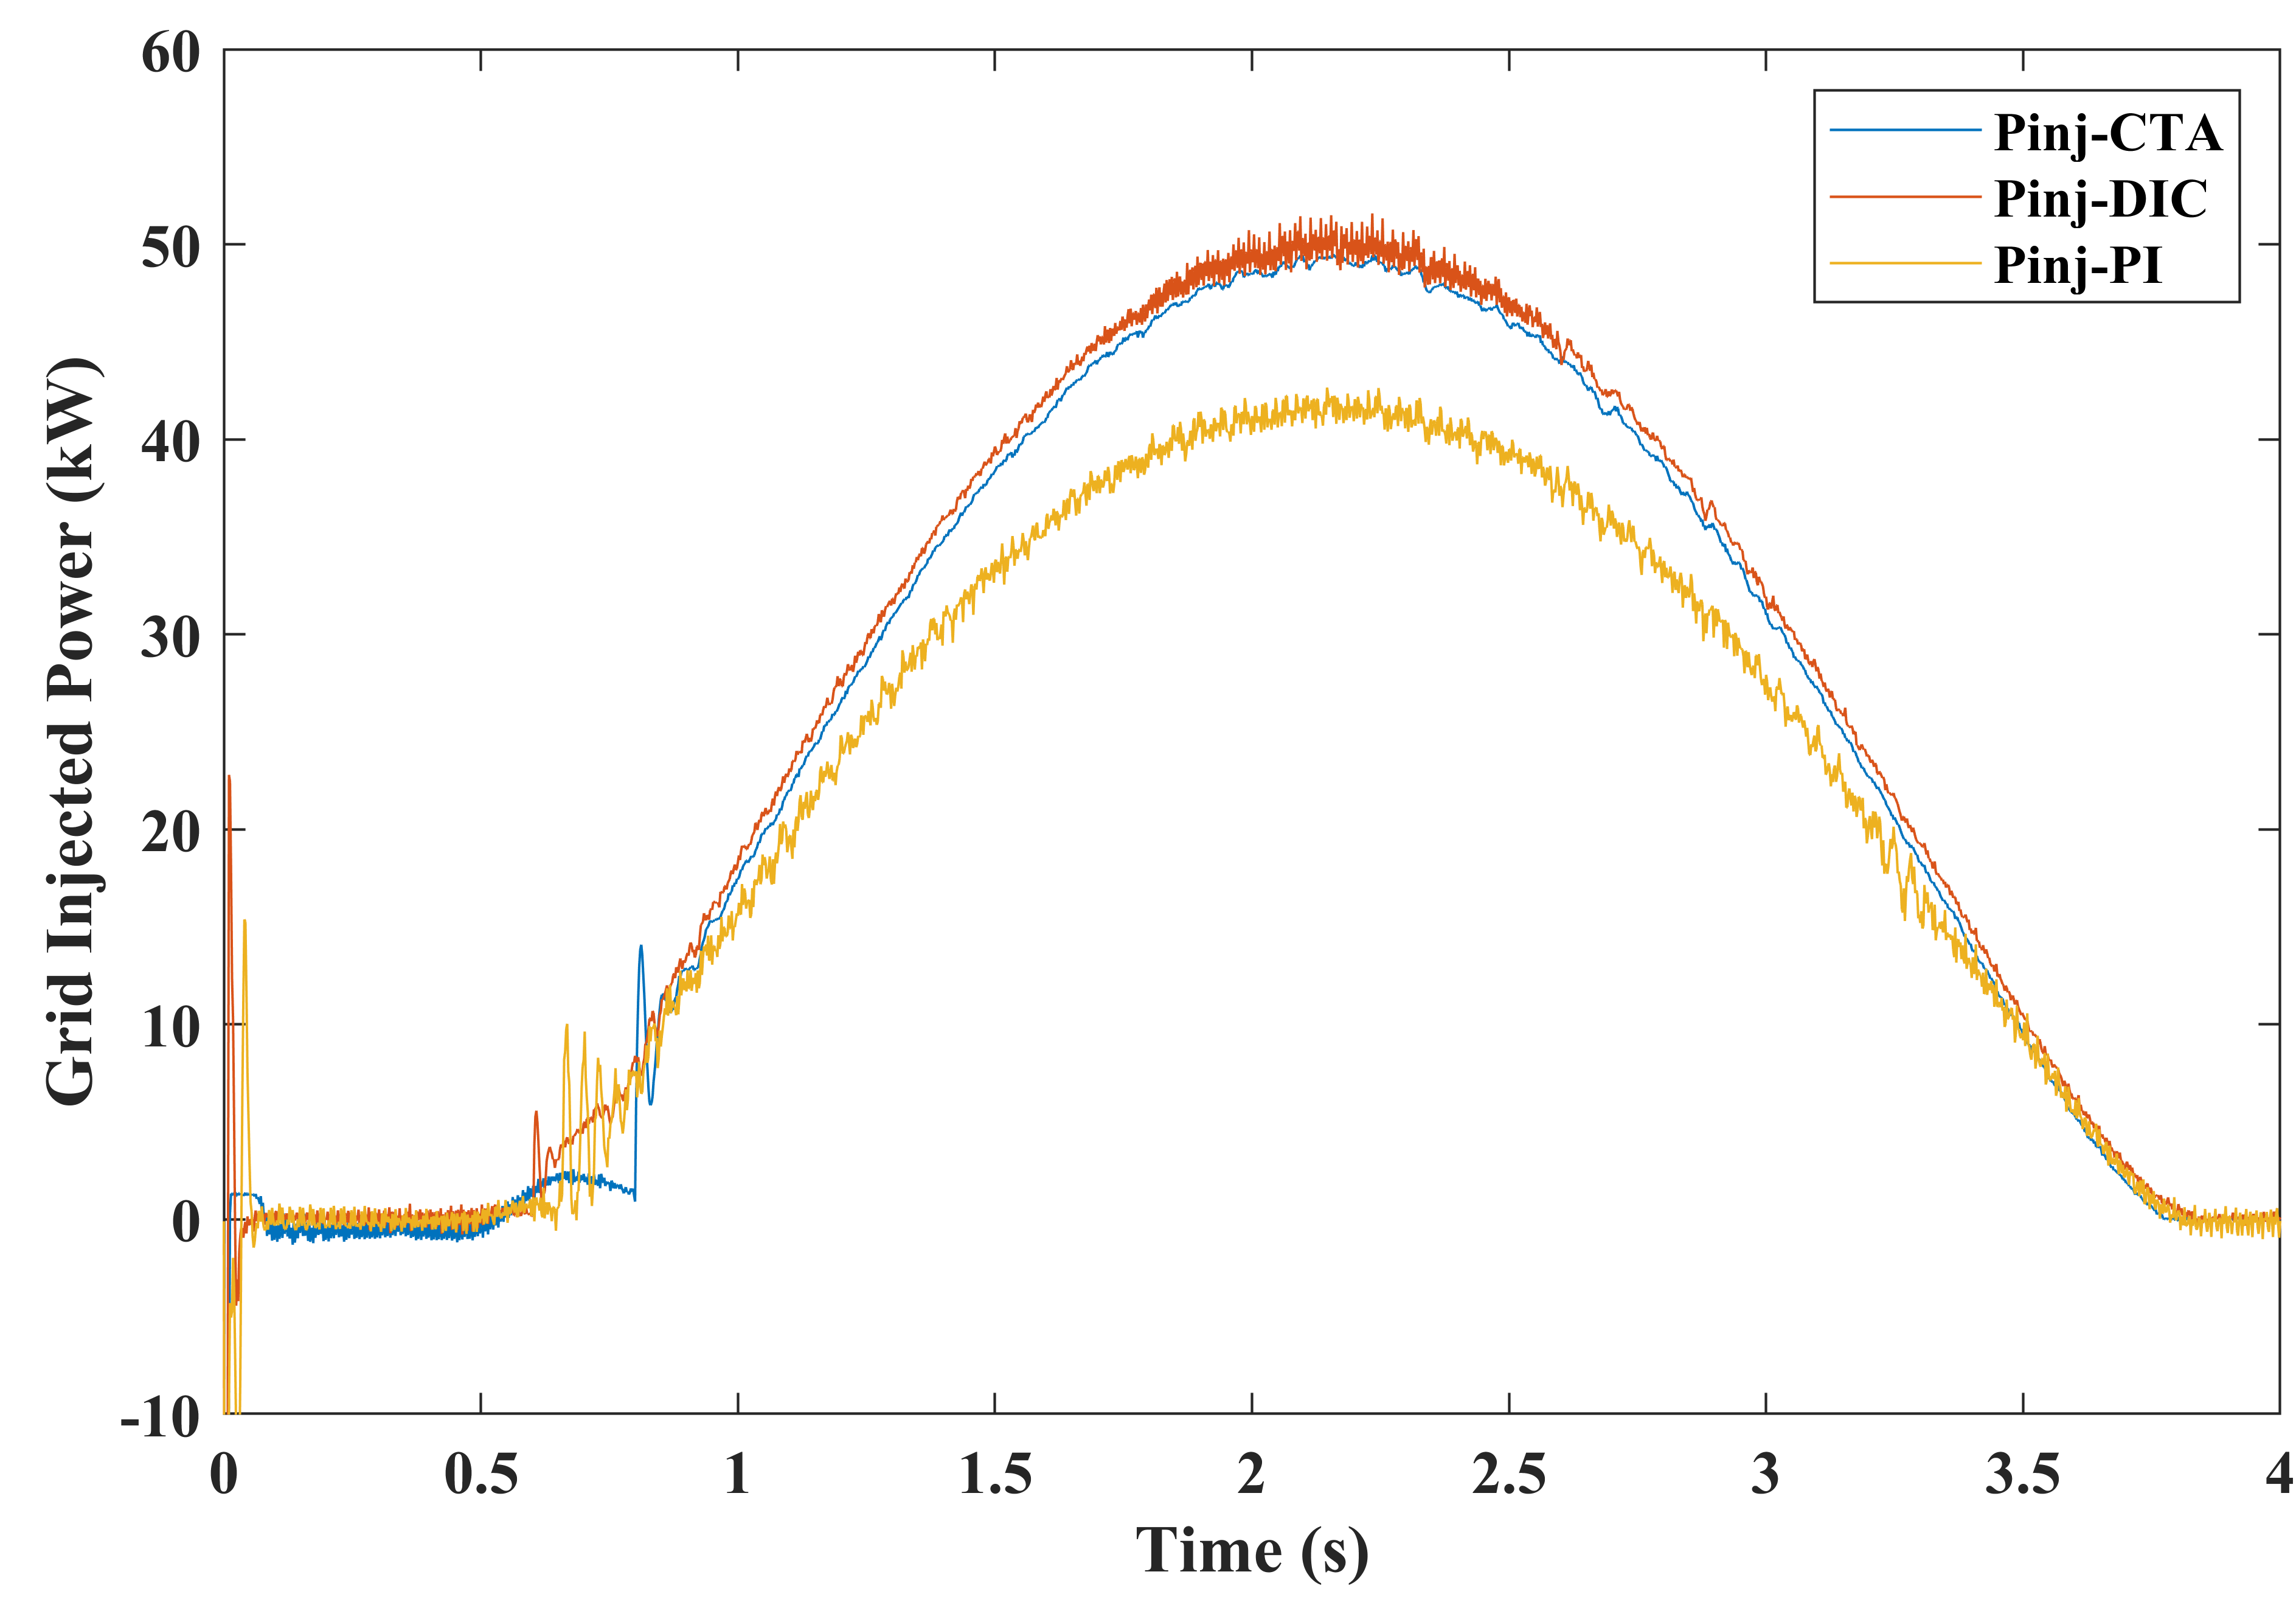
\includegraphics[width=\linewidth]{Pictures/Comparison Grid Inj Power.png}
\caption{Comparison of active power injected into the grid.}
\label{fig:grid-power-comparison}
\end{figure}

The performance indices are
\begin{equation}
J_{\mathrm{IAE}}=\int_{t_0}^{t_f}|e(t)|\,dt,\qquad
J_{\mathrm{ITAE}}=\int_{t_0}^{t_f}t|e(t)|\,dt,
\end{equation}
\begin{equation}
J_{\mathrm{ISE}}=\int_{t_0}^{t_f}e^2(t)\,dt,\qquad
J_{\mathrm{ITSE}}=\int_{t_0}^{t_f}te^2(t)\,dt.
\end{equation}
For MPPT, $e(t)=P_{\mathrm{ref}}(t)-P_{pv}(t)$.

\begin{table}[htbp]
\centering
\caption{MPPT efficiency and performance indices.}
\label{tab:mppt-indices}
\begin{tabular}{lccccc}
\toprule
Controller & Efficiency & IAE & ITAE & ISE & ITSE\\
\midrule
CTA & $99.4\%$ & 0.5750 & 2.2998 & 0.1375 & 0.5501\\
DIC & $98.0\%$ & 0.7596 & 3.0386 & 0.2283 & 0.9133\\
PI & $95.0\%$ & 2.6615 & 10.6461 & 5.6062 & 22.4250\\
\bottomrule
\end{tabular}
\end{table}

\begin{table}[htbp]
\centering
\caption{Grid-current THD and inverter tracking-error indices.}
\label{tab:inverter-indices}
\begin{tabular}{lccccc}
\toprule
Controller & THD & IAE & ITAE & ISE & ITSE\\
\midrule
CTA & $0.43\%$ & 0.6458 & 2.5917 & 1.3167 & 5.2668\\
DIC & $0.82\%$ & 1.2528 & 5.0262 & 5.4907 & 21.9627\\
PI & $2.27\%$ & 2.1180 & 8.4850 & 11.7053 & 46.8213\\
\bottomrule
\end{tabular}
\end{table}

The CTA provides the lowest MPPT and inverter error indices and the lowest reported current THD. The DIC also improves all reported metrics relative to the PI controller.

\section{Conclusion}
\label{sec:conclusion}

This study investigated CTA- and DIC-based control schemes for a two-stage grid-connected PV system. The controllers were applied to the boost converter for PV-voltage tracking and to the inverter for grid-current regulation. A P\&O algorithm generated the reference PV voltage, an outer PI loop generated the $d$-axis grid-current reference, and an Utkin observer reconstructed the filter-capacitor voltages and inverter-side currents.

Under varying irradiance, the CTA achieved a dynamic MPPT efficiency of $99.4\%$, compared with $98.0\%$ for the DIC and $95.0\%$ for the PI controller. The reported grid-current THD values were $0.43\%$, $0.82\%$, and $2.27\%$, respectively. The CTA also produced the lowest MPPT and inverter tracking-error indices. Under the stated assumptions, the controller structures provide finite-time MPPT error convergence and finite-time reaching of the inverter sliding manifolds, followed by exponential current-error convergence.

\subsection*{Limitations and Future Work}

The study is limited to MATLAB/Simulink simulations. The effects of measurement noise, parameter uncertainty, finite switching frequency, computation delay, quantization, and hardware constraints have not been experimentally verified. Future work will consider real-time and hardware-in-the-loop validation, unbalanced and faulted grid conditions, partial shading, controller-gain sensitivity, computational requirements, and experimental comparison with other nonlinear and predictive control methods.

\bibliographystyle{elsarticle-num}
\bibliography{references-reviewed}

\end{document}
